% !TeX program = xelatex
% =====================================================================
%  Anton Kapustin, "Langlands Duality and Topological Field Theory"
%  Caltech, February 15, 2010 — 中文译注本
%
%  导言区（由 main.tex 与 tools/checkbuild.ps1 共同 \input）
%  编译：xelatex（两遍），需 ctex（含 xeCJK）
% =====================================================================
\documentclass[11pt,a4paper,UTF8]{ctexart}

% ---------- 页面与版式 ----------
\usepackage[a4paper,left=2.6cm,right=2.6cm,top=2.6cm,bottom=2.8cm]{geometry}
\usepackage{fancyhdr}
\pagestyle{fancy}
\fancyhf{}
\fancyhead[L]{\small\itshape Langlands Duality and Topological Field Theory}
\fancyhead[R]{\small\thepage}
\renewcommand{\headrulewidth}{0.4pt}

% ---------- 数学 ----------
\usepackage{amsmath}
\usepackage{amssymb}
\usepackage{amsthm}
\usepackage{mathtools}
\usepackage{bm}

% ---------- 图形 ----------
\usepackage{graphicx}
\graphicspath{{fig/}{./fig/}}
\usepackage{xcolor}
\usepackage{booktabs}
\usepackage{array}
\usepackage{enumitem}
\usepackage{caption}
\captionsetup{font=small,labelsep=quad}
\setlength{\emergencystretch}{5em}

% ---------- 浮动体参数：避免整页只剩两张图、正文被推走 ----------
\renewcommand{\topfraction}{0.9}
\renewcommand{\bottomfraction}{0.8}
\renewcommand{\textfraction}{0.07}
\renewcommand{\floatpagefraction}{0.8}
\setcounter{topnumber}{3}
\setcounter{bottomnumber}{2}
\setcounter{totalnumber}{4}

% ---------- 超链接 ----------
\usepackage[colorlinks=true,linkcolor=blue!55!black,citecolor=blue!55!black,
            urlcolor=blue!55!black,unicode]{hyperref}

% ---------- 标题层级：原文用 0.1–0.10 编号 ----------
\renewcommand{\thesection}{0.\arabic{section}}

% ---------- 每节重点（Key Takeaways） ----------
% 说明：不用 minipage 包裹，以便允许跨页断开——否则恰在节首遇到整块不可分割的盒子时，
% TeX 会把整个节标题推到下一页，留下半页空白。
\newenvironment{keypoints}{%
  \par\addvspace{0.9em}%
  \noindent{\color{black!80}\rule{\linewidth}{0.6pt}}\par\nopagebreak\vspace{2pt}%
  \noindent\textbf{【本节重点】}\par\nopagebreak\vspace{2pt}%
  \begin{itemize}[leftmargin=1.6em,itemsep=1pt,topsep=2pt,parsep=0pt]%
}{%
  \end{itemize}\vspace{1pt}\noindent{\color{black!80}\rule{\linewidth}{0.6pt}}\par\addvspace{0.9em}%
}

\begin{document}

\begin{center}
  {\LARGE\bfseries 朗兰兹对偶与拓扑场论}\\[0.6em]
  {\large Anton Kapustin}\\[0.3em]
  {\normalsize California Institute of Technology, Pasadena, CA 91125, U.S.A.}\\[0.3em]
  {\normalsize 2010 年 2 月 15 日}
\end{center}

\vspace{0.4em}
\noindent\rule{\linewidth}{0.4pt}
\begin{center}
  \small 中文译注本：语义级翻译 + 公式逐符号校核 + 结构化 \LaTeX{} 源码 + 学术批注\\
  \small 原文：Anton Kapustin, \emph{Langlands Duality and Topological Field Theory}, 2010（Preprint）
\end{center}
\noindent\rule{\linewidth}{0.4pt}

\vspace{0.6em}
\begin{keypoints}
    \item \textbf{阅读提示：}每节开头给出“本节重点”。源码中以 \verb|% [Tutor Note: ...]| 形式出现的注释是学术审校批注，编译后不显示，供阅读源码者参考。
    \item \textbf{符号约定：}全文沿用原文记号（$G$、${}^{L}G$、$\tau$、$e^{2}$、$\theta$、$t$、$\Psi$、$\omega_{K}$ 等），未作重新定义。
    \item \textbf{编号约定：}节号沿用原文 0.1–0.10；公式编号沿用原文 (1)–(6)；参考文献编号沿用原文 [1]–[49]；脚注 1–10 顺序不变。
\end{keypoints}

% [Tutor Note: 排印层面的统一处理（不影响任何数学内容），共三条，便于教授核对本译本与原文的差异：
%  (1) 原文把群名 SU、SO、Sp、Spin、PSL、SL、U 及例外群 E8、F4、G2 一律排成数学斜体（PDF 内字体为 CMMI10），
%      本译本统一改为正体 \mathrm{}。理由：正体是当代文献的通行排法，且能把群名与同名变量（如 $G$、$R$）区分开；
%      若需与原文版式完全一致，只需全局把 \mathrm{SU} 等改回裸字母即可。
%  (2) Hodge 星算子原文用 ⋆（\star），本译本同；微分符号原文用斜体 d，本译本统一改为正体 \mathrm{d}，
%      以免与变量 d 混淆——这一改动在涉及 \mathrm{d} 与 \star 同时出现的外微分、Bianchi 恒等式处最需注意。
%  (3) 原文（以及本节若干处）用 “∧” 表示外积、用 “·” 表示算子复合，均照原文保留。
% 上述三条均只涉及字体与符号排版，未改动任何上下标、指标位置或公式结构。]

\clearpage

% ==================================================================
%  片段 s01.tex
% ==================================================================
% [Tutor Note: 本片段对应原文 p2–p6：0.1 引言（p2）与 0.2 阿贝尔规范场论中的电–磁对偶（p2 末–p6 首）。
%  这两节原文均无脚注（脚注 1 从 p7 的 0.3 节开始），故本片段不含 \footnote。全片段只有式 (1) 一个编号公式。]

\section{引言}

\begin{keypoints}
    \item \textbf{物理图像：}朗兰兹纲领讨论绝对伽罗瓦群的表示；Drinfeld 与 Laumon 的几何类比把“基本群表示”换成“基本群到复约化李群的同态”，即曲面上的平坦联络。
    \item \textbf{数学工具：}几何朗兰兹对偶把不可约平坦 $G_{\mathbb{C}}$-联络对应为全纯 ${}^{L}G$-丛模叠上的 $D$-模；对偶群 ${}^{L}G$ 由“同态格与权格互换”的根数据对偶定义。
    \item \textbf{关键结论：}$\mathrm{SU}(N)$ 的对偶是 $\mathrm{SU}(N)/\mathbb{Z}_{N}$，$\mathrm{Sp}(N)$ 的对偶是 $\mathrm{SO}(2N+1)$，而 $\mathrm{U}(N)$、$\mathrm{E}_{8}$、$\mathrm{F}_{4}$、$\mathrm{G}_{2}$ 自对偶。
    \item \textbf{物理动机：}Goddard–Nuyts–Olive 的磁源分类（磁源按 ${}^{L}G$ 的不可约表示分类）导出 Montonen–Olive 猜想；Osborn 指出 $\mathcal{N}=4$ 超对称版本更可能成立。
\end{keypoints}

朗兰兹纲领（Langlands Program）是关于某些域的绝对伽罗瓦群表示的一大类定理与猜想的统称；近期的一份通俗综述见 [1]。V. Drinfeld 与 G. Laumon [2] 引入了一个几何类比，其中讨论的是黎曼曲面 $C$ 的基本群的表示，或者更一般地，是从 $\pi_{1}(C)$ 到约化代数李群 $G_{\mathbb{C}}$ 的同态的等价类（我们把 $G_{\mathbb{C}}$ 看成紧约化李群 $G$ 的复化）。从几何的观点看，这样的同态对应于 $C$ 上某个主 $G_{\mathbb{C}}$ 丛上的平坦联络。

% [Tutor Note: p2 第 1 段。${}^{L}G$ 的定义必须连同根系一起理解：原文说“从 $\mathrm{U}(1)$ 到极大环面的同态格”，即余权格
%  $X_{*}(T_{G})=\mathrm{Hom}(\mathrm{U}(1),T_{G})$，条件是它与 ${}^{L}G$ 的权格同构；等价地，${}^{L}G$ 的余权格是 $G$ 的权格。
%  也就是把根数据取对偶（根系与余根系互换）。只记住“权格与余权格互换”而漏掉根系，容易把 $\mathrm{SU}(N)$ 的对偶误写成
%  $\mathrm{SU}(N)$ 本身；正确结果是中心 $\mathbb{Z}_{N}$ 与平凡群互换的 $\mathrm{SU}(N)/\mathbb{Z}_{N}$。另注意 ${}^{L}G$ 按原文取紧形式，
%  不要与复化群 $G_{\mathbb{C}}$ 混淆。]

几何朗兰兹对偶把不可约平坦 $G_{\mathbb{C}}$-联络对应为 $C$ 上全纯 ${}^{L}G$-丛的模叠上的某个 $D$-模。这里 ${}^{L}G$ 一般是另一个紧约化李群，称为 $G$ 的朗兰兹对偶群。群 ${}^{L}G$ 由如下条件定义：从 $\mathrm{U}(1)$ 到 $G$ 的极大环面的同态所构成的格，同构于 ${}^{L}G$ 的权格。例如，$\mathrm{SU}(N)$ 的对偶是 $\mathrm{SU}(N)/\mathbb{Z}_{N}$，$\mathrm{Sp}(N)$ 的对偶是 $\mathrm{SO}(2N+1)$，而群 $\mathrm{U}(N)$、$\mathrm{E}_{8}$、$\mathrm{F}_{4}$、$\mathrm{G}_{2}$ 都是自对偶的。

李群的同一种对偶概念也出现在 P. Goddard、J. Nuyts 与 D. Olive 关于规范理论中磁源分类的工作 [3] 中。他们发现，规范群为 $G$ 的规范理论中的磁源，由对偶群 ${}^{L}G$ 的不可约表示来分类。在此基础上，C. Montonen 与 D. Olive 猜测 [4]：规范群分别为 $G$ 与 ${}^{L}G$ 的杨–米尔斯理论在量子层面可能是同构的。这一猜想可以看作量子麦克斯韦理论中电–磁对偶的推广。后来 H. Osborn [5] 注意到，蒙托宁–奥利夫猜想更可能在杨–米尔斯理论的 $\mathcal{N}=4$ 超对称版本中成立。目前已有大量间接证据支持 MO 猜想，但还没有证明。

% [Tutor Note: p2 第 3 段。GNO 结论的推导线索：Dirac 量子化把磁荷限制在与电荷配对的那个格上，这个格正是 ${}^{L}G$ 的权格，
%  于是磁源的荷标号（从而其分类）由 ${}^{L}G$ 的不可约表示给出；原文只给结论，推导见 [3]。关于 Osborn 的 $\mathcal{N}=4$ 论点，
%  原文也没有展开：$\mathcal{N}=4$ 杨–米尔斯是有限理论（β 函数为零），耦合不随能标跑动，强、弱耦合的精确互换才可能成立；
%  非超对称情形没有这种保护。]

在 Goddard、Nuyts 与 Olive 的工作之后不久，M. Atiyah 就提出朗兰兹对偶可能与 MO 对偶有关；但直到最近才找到精确的联系 [6]。在这些讲座中，我将尝试解释 [6] 的主要思想；详细推导与更完整的参考文献列表，读者可参阅原始论文 [6]。本文不讨论几何朗兰兹对偶的带分歧（ramified）版本；关于这一点，读者可参阅 [7, 8, 9]。

% [Tutor Note: p2 第 4 段。原文的 "the original paper" 指 [6]，即文献表中的 Kapustin–Witten《Electric-Magnetic Duality and the Geometric
%  Langlands Program》，本讲义后文都在展开这篇文章。Atiyah 的提示远早于精确对应，原文未说明其依据；"ramified version" 本译作
%  “带分歧的版本”，对应 [7, 8, 9]，本讲义不涉及。]

\section{阿贝尔规范场论中的电–磁对偶}

\begin{keypoints}
    \item \textbf{物理图像：}无源 $\mathrm{U}(1)$ 麦克斯韦理论中，运动方程 $\mathrm{d}\star F=0$ 与 Bianchi 恒等式 $\mathrm{d}F=0$ 在 $F\mapsto\star F$ 下互换；经典层面的 $E\leftrightarrow B$ 交换是电–磁对偶的原型。
    \item \textbf{数学工具：}把对 $A$ 的路径积分改写为对“满足周期量子化条件的闭 2-形式 $F$”的积分，再引入 1-形式 $B$ 作拉格朗日乘子以实现 $\delta(\mathrm{d}F)$，最后用高斯积分完成对 $F$ 的积分。
    \item \textbf{关键结论：}对偶后配分函数形式不变，耦合与 $\theta$ 角互换；复参数 $\tau=\frac{\theta}{2\pi}+\frac{2\pi i}{e^{2}}$ 变为 $\tau\mapsto-\frac{1}{\tau}$，$\mathrm{U}(1)$ 情形下强弱耦合互换不带来困难。
    \item \textbf{关键机制：}量子理论中对丛 $E$ 的所有拓扑求和，使对偶在任意 $X$ 上恢复；$\theta\mapsto\theta+2\pi$ 的平移在自旋流形上是对称性，与 $\tau\mapsto\tau+1$ 一起生成 $\mathrm{PSL}(2,\mathbb{Z})$。
\end{keypoints}

我先回顾麦克斯韦理论中的电–磁对偶。麦克斯韦理论是无源的 $\mathrm{U}(1)$ 规范场论。在经典层面，该理论描述四维流形 $X$ 上主 $\mathrm{U}(1)$ 丛 $E$ 上的一个联络 $A$。假定四维流形 $X$ 配有洛伦兹号差度规（稍后我们将换用黎曼号差）。$A$ 的运动方程为
\[
    \mathrm{d}\star F = 0,
\]
其中 $F=\mathrm{d}A$ 是 $A$ 的曲率，$\star$ 是作用在形式上的 Hodge 星算子。此外，曲率 2-形式 $F$ 是闭的：$\mathrm{d}F=0$（这称为 Bianchi 恒等式），因此可以在很大程度上用 $F$ 取代 $A$（消去 $A$）。更准确地说，$F$ 决定了 $A$ 沿 $X$ 中所有可缩闭路的和乐（holonomy）。若 $\pi_{1}(X)$ 平凡，则 $F$ 完全决定 $A$（在规范等价意义下）。此外，若 $H^{2}(X)\neq 0$，$F$ 还要满足量子化条件：它的周期是 $2\pi$ 的整数倍。$F$ 的上同调类是 $E$ 的 Euler 类（或者等价地，是相伴线丛的第一陈类）。

% [Tutor Note: p3 第 1 段。"eliminate $A$ in favor $F$" 原文漏了 of，应为 in favor of $F$；这是原文排印疏漏，译文按语义处理，
%  未改动数学内容。另注意这里的逻辑：$F$ 只在 $X$ 单连通时才完全决定 $A$（相差规范）；当 $H^{2}(X)\neq 0$ 时 $F$ 的周期提供额外
%  离散数据，而 $\star F$ 一般不再满足 $2\pi$ 量子化，这正是经典对偶在一般 $X$ 上失效的原因（下文 p3 末–p4 开头说明量子层面如何恢复）。]

当 $X=\mathbb{R}^{3,1}$ 时，该理论显然在下述变换下不变：
\begin{equation}
    F \mapsto F' = \star F. \tag{1}
\end{equation}
若 $X$ 为洛伦兹号差，则该变换的平方为 $-1$。它称为电–磁对偶。为理解其中缘由，设 $x^{0}$ 为类时坐标，$x^{i}$（$i=1,2,3$）为类空坐标。则通常的电场与磁场为
\[
    E_{i}=F_{0i},\qquad B_{i}=\frac{1}{2}\epsilon_{ijk}F_{jk},
\]
而变换 (1) 的作用为
\[
    E_{i}\mapsto B_{i},\qquad B_{i}\mapsto -E_{i}.
\]
因此，在相差若干符号的意义下，该对偶变换交换电场与磁场。这些符号是为了与洛伦兹变换相容所必需的。换个角度，从哈密顿形式的角度看，这些符号是为了保持场 $E_{i}$ 与 $B_{i}$ 构成的空间上的辛结构所必需的。该辛结构对应于泊松括号
\[
    \{B_{i}(x),E_{k}(y)\}=\frac{e^{2}}{2}\epsilon_{ijk}\partial_{j}\delta^{3}(x-y),
\]
其中 $e^{2}$ 是耦合常数（它决定作用量的整体归一化）。

% [Tutor Note: p3 式 (1) 与“平方为 $-1$”。在四维洛伦兹号差下，2-形式上的 Hodge 星满足 $\star^{2}=-1$，所以 $F\mapsto\star F$
%  作用两次等于 $-1$；这正是 p5 末至 p6 说“作用两次给出 $-1$”、并把对偶群取为 $\mathrm{SL}(2,\mathbb{Z})$ 双覆盖的原因。
%  从 p4 起改用欧氏号差后，2-形式上有 $\star^{2}=+1$，同一个 $\star$ 不再具有“旋转”的含义，对偶关系式中出现的因子 $i$
%  （如 p5 的 $F=ie^{2}\star G$）正是号差改变留下的痕迹。核对 $\star^{2}$ 时必须同时确认度规号差与 $\star$ 的定义
%  （是否含 $i$、是否用 $\alpha\wedge\star\beta=\langle\alpha,\beta\rangle\mathrm{vol}$ 的约定）。]

% [Tutor Note: p3 泊松括号的系数。由正则量子化 $\{A_{i}(x),E^{j}(y)\}=e^{2}\delta_{i}^{j}\delta^{3}(x-y)$ 与
%  $B_{i}=\frac{1}{2}\epsilon_{ijk}F_{jk}=\epsilon_{ijk}\partial_{j}A_{k}$ 直接推算，得到
%  $\{B_{i}(x),E_{k}(y)\}=e^{2}\epsilon_{ijk}\partial_{j}\delta^{3}(x-y)$，系数应为 $e^{2}$；原文写作 $\frac{e^{2}}{2}$，
%  疑为笔误或某处未说明的归一化约定。此处按页面图像原样誊写，未擅改。另注意指标：左端 $i,k$ 固定，$\epsilon_{ijk}$ 对 $j$ 缩并，
%  $\partial_{j}$ 作用在 $\delta^{3}$ 上。]

如上所述，只有在单连通的流形上，经典理论才能完全用 $F$ 重写。此外，与 $F$ 不同，$\star F$ 不必满足任何量子化条件。因此看起来，在比 $\mathbb{R}^{3,1}$ 更复杂的流形上对偶并不存在。有趣的是，在量子理论中，只要对所有丛 $E$ 的拓扑求和，对偶对任意 $X$ 都能恢复。为看清这一点，回想量子理论由其路径积分定义：
\[
    Z=\int \mathcal{D}A\, e^{iS(A)},
\]
其中 $S(A)$ 是作用量泛函。我们取作用量为
\[
    S(A)=\frac{1}{2e^{2}}\int_{X}F\wedge\star F+\frac{\theta}{8\pi^{2}}\int_{X}F\wedge F .
\]
它的临界点恰为 $\mathrm{d}\star F=0$ 的解。注意作用量中的第二项只依赖于 $E$ 的拓扑，因此不影响经典运动方程；但它影响作用量，因而在量子理论中必须予以考虑。事实上，若对所有 $E$ 的同构类求和，即把路径积分定义为
\[
    Z=\sum_{E}\int \mathcal{D}A\, e^{iS(A)},
\]
则参数 $\theta$ 告诉我们如何对不同 $E$ 的贡献加权。

% [Tutor Note: p4 作用量第二项的归一化。$F$ 的周期为 $2\pi$ 的整数倍，故 $\int_{X}F\wedge F=4\pi^{2}c_{1}^{2}$（$c_{1}$ 为第一陈类），
%  于是 $\frac{\theta}{8\pi^{2}}\int F\wedge F=\frac{\theta}{2}c_{1}^{2}$；这正是 p5 中“$\theta$ 是拓扑项 $-\frac{i}{2}c_{1}^{2}$ 的系数”的由来。
%  不同文献对 $\theta$ 项常用 $\frac{\theta}{8\pi^{2}}\mathrm{Tr}F\wedge F$、$\frac{\theta}{32\pi^{2}}\mathrm{Tr}F\wedge F$ 等不同归一化，
%  换算时若漏掉 $4\pi^{2}$ 或 $\mathrm{Tr}$ 的因子，$\tau$ 的定义就会错，务必按 $1/8\pi^{2}$ 核对。]

到这一步，把 $X$ 换成黎曼流形（我们仍记作 $X$）非常方便。这里的想法是：洛伦兹号差流形上的路径积分应当定义为欧氏号差下路径积分的解析延拓；这称为 Wick 转动。在欧氏号差下，路径积分与作用量看起来略有不同：
\[
    Z=\sum_{E}\int \mathcal{D}A\, e^{-S_{E}(A)},
\]
其中
\[
    S_{E}(A)=\int_{X}\left(\frac{1}{2e^{2}}F\wedge\star F-\frac{i\theta}{8\pi^{2}}F\wedge F\right).
\]
注意在欧氏号差下作用量变成复的。

% [Tutor Note: p4 Wick 转动后的符号。欧氏作用量里 $\theta$ 项带 $-i$（Minkowski 作用量中为 $+\frac{\theta}{8\pi^{2}}\int F\wedge F$），
%  配分函数的权重从 $e^{iS}$ 换成 $e^{-S_{E}}$；这两处符号必须一起换，否则 $\tau$ 实部（即 $\theta$ 项）的符号会反。
%  欧氏号差下 $S_{E}$ 不是实泛函，这是 $\theta$ 项造成的，不是笔误。]

现在勾勒量子层面上的对偶如何产生。为简单起见，假设 $X$ 单连通，于是可以把对 $A$ 的积分换成对满足周期量子化条件的闭 2-形式 $F$ 的积分。若进一步假设 $X=\mathbb{R}^{4}$，量子化条件为空，配分函数可写成
\[
    Z=\int \mathcal{D}F\,\mathcal{D}B\, \exp\left(-S_{E}+i\int_{X}B\wedge\mathrm{d}F\right).
\]
这里新场 $B$ 是 $X$ 上的 1-形式；引入它是为了使对 $B$ 的积分给出 $\delta$-泛函 $\delta(\mathrm{d}F)=\prod_{x\in X}\delta(\mathrm{d}F(x))$。这使我们能对一切（不必闭的）2-形式 $F$ 积分。

现在利用这是高斯积分来对 $F$ 积分，结果为
\[
    Z=\int \mathcal{D}B\, \exp\left(-\frac{1}{2\hat{e}^{2}}\int_{X}G\wedge\star G+\frac{i\hat{\theta}}{8\pi^{2}}\int_{X}G\wedge G\right),
\]
其中 $G=\mathrm{d}B$，而参数 $\hat{e}^{2}$ 与 $\hat{\theta}$ 由下式定义：
\[
    \frac{\hat{\theta}}{2\pi}+\frac{2\pi i}{\hat{e}^{2}}=-\left(\frac{\theta}{2\pi}+\frac{2\pi i}{e^{2}}\right)^{-1}.
\]

% [Tutor Note: p4 的高斯积分。把 $-S_{E}(F)+i\int B\wedge\mathrm{d}F$ 对 $F$ 配方：$F\wedge\star F$ 项给出对偶作用量的
%  $\frac{1}{2\hat{e}^{2}}G\wedge\star G$，$F\wedge F$ 项给出 $\frac{i\hat{\theta}}{8\pi^{2}}G\wedge G$，交叉项与 $B\wedge\mathrm{d}F$ 合并后消去；
%  行列式因子是与场无关的常数，不影响对偶关系的读出。注意 $F$ 与 $G=\mathrm{d}B$ 同为 2-形式，$\star$ 在四维作用在 2-形式上。
%  原文直接写出结果，未展示配方过程；上式右端的负号与逆矩阵是关键：它等价于 $\hat{\tau}=-\frac{1}{\tau}$。]

我们看到，以 $B$ 的积分写出的配分函数，与以 $A$ 的积分写出的配分函数形式完全相同，只是 $e^{2}$ 与 $\theta$ 换成了 $\hat{e}^{2}$ 与 $\hat{\theta}$。这正是电–磁对偶的体现。为更清楚地看到这一点，注意当 $\theta=0$ 时，由作用量
\[
    S_{E}(F)-i\int_{X}B\wedge\mathrm{d}F
\]
推出的 $F$ 的运动方程为
\[
    F=ie^{2}\star G .
\]
因子 $i$ 来自度规的黎曼号差；在洛伦兹号差下做类似运算会得到相同的公式，但没有 $i$。

% [Tutor Note: p5 的 $F=ie^{2}\star G$。这个 $i$ 完全是欧氏号差的产物（洛伦兹号差下没有 $i$）；与式 (1) 对照可见，
%  它就是经典关系 $F\propto\star G$ 的欧氏版本。本式由 p5 的指数 $-S_{E}+i\int B\wedge\mathrm{d}F$ 对 $F$ 变分得到（取 $\theta=0$），
%  变分时 $\mathrm{d}F$ 要分部积分到 $B$ 上，从而出现 $G=\mathrm{d}B$。]

上述电–磁对偶的推导只在 $X$ 拓扑平凡时成立。若 $H^{2}(X)\neq 0$，就必须在 $F$ 与 $B$ 的路径积分中插入额外的 $\delta$-泛函，以保证 $F$ 的周期被正确量子化。结果表明，这些 $\delta$-泛函的效果可以通过让 $B$ 成为 $X$ 上任一主 $\mathrm{U}(1)$ 丛 $\hat{E}$ 上的联络 1-形式、并对所有可能的 $\hat{E}$ 求和来重现。对一般四维流形 $X$ 成立的证明见 [10]。

% [Tutor Note: p5 第 3 段。原文 "by letting $B$ to be a connection 1-form" 中 "to be" 多余，应为 "letting $B$ be"。
%  物理上这一步与 p4 的 $\sum_{E}$ 相呼应：对偶之后，求和的拓扑对象从电丛 $E$ 换成磁丛 $\hat{E}$，所以对 $\hat{E}$ 的求和
%  正是“磁拓扑”的求和；一般流形上的严格证明见 [10]（Witten 关于阿贝尔规范理论 S-对偶的文章）。]

从这个推导可以看出，对偶对耦合 $e^{2}$ 与参数 $\theta$ 的作用是非平凡的。为描述这一作用，方便的做法是引入取值于上半平面的复参数 $\tau$：
\[
    \tau=\frac{\theta}{2\pi}+\frac{2\pi i}{e^{2}} .
\]
于是电–磁对偶的作用为
\[
    \tau\to-\frac{1}{\tau}.
\]
注意，若 $X$ 是自旋流形，则变换 $\tau\to\tau+1$（等价地，$\theta\to\theta+2\pi$）也是理论的对称性。确实，$\theta$ 以拓扑项
\[
    -\frac{i}{2}c_{1}^{2}
\]
的系数形式进入作用量，其中 $c_{1}$ 是 $E$ 的第一陈类。若 $X$ 是自旋流形，则任意整上同调类的平方可被 $2$ 整除，于是上述拓扑项是 $i$ 的整数倍。这立刻推出：把 $\theta$ 平移 $2\pi$ 不改变 $e^{-S_{E}}$。（对任意 $X$，变换 $\tau\to\tau+2$ 仍是理论的对称性。）

% [Tutor Note: p5 的 $\tau$ 定义。本讲义 $\operatorname{Im}\tau=\frac{2\pi}{e^{2}}$；由于 $e^{2}>0$，故 $\operatorname{Im}\tau>0$，
%  这就是 $\tau$ 取值于上半平面的原因。许多文献（例如 $\mathcal{N}=2$ 超对称规范理论）用 $\tau=\frac{\theta}{2\pi}+\frac{4\pi i}{g^{2}}$，
%  与本讲义的虚部相差因子 $2$（视作用量归一化与 $\mathrm{Tr}$ 的约定而定）。比较不同文献的 $S$-对偶公式前必须先对齐 $\tau$ 的定义，
%  否则 $\hat{e}^{2}$ 与 $e^{2}$ 的换算会整体差一个因子。]

% [Tutor Note: p5 自旋条件与拓扑项。作用量中与 $\theta$ 有关的部分为 $-\frac{i\theta}{2}c_{1}^{2}$；把它看成 $-\frac{i}{2}c_{1}^{2}$ 的
%  $\theta$ 倍，即原文所说“$\theta$ 作为该拓扑项的系数”。自旋流形上 $c_{1}^{2}$ 为偶数，故 $-\frac{i}{2}c_{1}^{2}$ 是 $i$ 的整数倍；
%  $\theta\to\theta+2\pi$ 使作用量改变 $-\pi i\,c_{1}^{2}=-2\pi i\,m$，是 $2\pi i$ 的整数倍，故 $e^{-S_{E}}$ 不变。
%  对非自旋的 $X$，$c_{1}^{2}$ 可为奇数，只有 $\theta\to\theta+4\pi$（即 $\tau\to\tau+2$）才保证不变。
%  注意 $c_{1}^{2}$ 指 $\int_{X}c_{1}\wedge c_{1}$，不是逐点的乘积。]

变换 $\tau\to-\frac{1}{\tau}$ 与 $\tau\to\tau+1$ 生成了作用在上半平面上的整系数分式线性变换的整群，即群 $\mathrm{PSL}(2,\mathbb{Z})$。上半平面中由 $\mathrm{PSL}(2,\mathbb{Z})$ 相联系的点给出同构的理论。这个群可以称为对偶群。实际上，把这个名字留给它的“双覆盖” $\mathrm{SL}(2,\mathbb{Z})$ 更好，因为把电–磁对偶作用两次会作用在 2-形式 $F$ 上产生 $-1$。在这些讲座中，我们将主要关注电–磁对偶，它是 $\mathrm{SL}(2,\mathbb{Z})$ 的一个特定元素，也称为 S-对偶。注意当 $\theta=0$ 时，S-对偶交换弱耦合（$e^{2}\ll 1$）与强耦合（$e^{2}\gg 1$）。这在阿贝尔情形不会带来麻烦，因为对任意耦合值我们都能解出 $\mathrm{U}(1)$ 规范理论；但在非阿贝尔情形它会使问题大大复杂化，因为那里的理论只对小 $e^{2}$ 可解。

% [Tutor Note: p5 末至 p6 的对偶群。$\mathrm{SL}(2,\mathbb{Z})$ 与 $\mathrm{PSL}(2,\mathbb{Z})$ 的差别正是中心元 $-1$：$\tau$ 只感受到
%  $\mathrm{PSL}(2,\mathbb{Z})$（分式线性变换在 $\tau$ 上 $-\mathrm{id}$ 与 $\mathrm{id}$ 作用相同），但场 $F$ 在两次对偶后变号
%  （洛伦兹号差下 $\star^{2}=-1$），所以完整作用在 $(F,\tau)$ 上的是 $\mathrm{SL}(2,\mathbb{Z})$。这就是原文说“把 duality group
%  留给双覆盖”的含义。S-对偶对应 $\tau\to-\frac{1}{\tau}$；在 $\theta=0$ 时由 p4 末的参数关系可得 $\hat{e}^{2}=\frac{4\pi^{2}}{e^{2}}$，
%  故 $e^{2}\ll 1$ 与 $e^{2}\gg 1$ 互换。]

% [Tutor Note: 原文排印疏漏（照译，不改正）：p6 首行 "In this lectures" 应为 "In these lectures"；
%  p5 "the transformations ... generated the whole group" 应为 "generate"；p3 与 p4 把 Lorentz 拼作 "Lorenz"
%  （"Lorenzian metric"、"Lorenz transformations"）；p5 "letting B to be" 多一个 "to be"（已在前文注明）。
%  这些都不影响数学内容。]

% ==================================================================
%  片段 s02.tex
% ==================================================================
\section{蒙托宁–奥利夫对偶}

\begin{keypoints}
    \item \textbf{物理图像：}把 Maxwell 理论中的电–磁对偶推广到非阿贝尔规范场。Goddard–Nuyts–Olive 指出磁源由另一个群（朗兰兹对偶群 ${}^{L}G$）的不可约表示标记；蒙托宁–奥利夫猜想 $G$ 与 ${}^{L}G$ 的量子理论同构，并交换电、磁源。
    \item \textbf{数学工具：}主丛联络 $A$ 与曲率 $F=\mathrm{d}A+A\wedge A$、协变微分 $\mathrm{d}_{A}$、Hodge 星 $\star$；余权格与权格互为对偶、外尔群作用、${}^{L}G$ 的最高权分类。
    \item \textbf{关键结论：}$\theta=0$ 时对偶耦合由式 (3) 给出，交换强弱耦合；引入 $\tau=\theta/(2\pi)+4\pi i/e^{2}$ 后，MO 对偶的作用是式 (4)，它与 $\tau\mapsto\tau+k$ 一起生成 $\mathrm{SL}(2,\mathbb{R})$ 的某个子群。
    \item \textbf{局限与修正：}纯杨–米尔斯理论中 $e$ 会被重整化，式 (3) 与重整化不相容，故 MO 对偶并不成立；$\mathcal{N}=4$ 超杨–米尔斯理论的规范耦合在任何微扰阶都不重整化，Osborn 又论证磁单极孤子与规范玻色子量子数完全相同，MO 对偶才成为可信的猜想。
    \item \textbf{通向下一节：}MO 对偶把超荷乘以依赖于 $\tau$ 的相位 $e^{\pm i\phi/2}$，$e^{i\phi}=|\tau|/\tau$；这一相位决定了 0.4 节中 $t$ 的变换，是几何朗兰兹对偶的根源。
\end{keypoints}

现在我们把上述考虑推广到非阿贝尔规范理论，也就是杨–米尔斯理论。基本场是四维流形 $X$ 上主 $G$-丛 $E$ 的联络 $A=A_{\mu}\mathrm{d}x^{\mu}$。四维流形 $X$ 配备一个洛伦兹度规 $g$，运动方程读作
\[
    \mathrm{d}_{A}F=0,\qquad \mathrm{d}_{A}\star F=0,
\]
其中 $F=\mathrm{d}A+A\wedge A\in\Omega^{2}(\operatorname{ad}(E))$ 是 $A$ 的曲率，$\mathrm{d}_{A}$ 是协变微分，$\star$ 是 $X$ 上的 Hodge 星算子。其中第一个方程恒成立，第二个方程则由变分杨–米尔斯作用量得到：
\[
    S(A)=\int_{X}\left(\frac{1}{2e^{2}}\operatorname{Tr}F\wedge\star F+\frac{\theta}{8\pi^{2}}\operatorname{Tr}F\wedge F\right).
\]
相应的欧氏作用量为
\[
    S_{E}(A)=\int_{X}\left(\frac{1}{2e^{2}}\operatorname{Tr}F\wedge\star F-i\frac{\theta}{8\pi^{2}}\operatorname{Tr}F\wedge F\right).
\]
% [Tutor Note: 见 p.6 运动方程与作用量。$\mathrm{d}_{A}F=0$ 是 Bianchi 恒等式（由 $F=\mathrm{d}A+A\wedge A$ 恒成立），并非独立场方程；独立的只有 $\mathrm{d}_{A}\star F=0$。从 Minkowski 号差转到欧氏号差时，$e^{iS}\to e^{-S_{E}}$ 会带来一个因子 $i$，所以 $\theta$ 项在 $S_{E}$ 中变为 $-i\theta/(8\pi^{2})$，符号不能丢。$\theta$ 项的归一化 $1/(8\pi^{2})$ 不是任意的：它使 $\int_{X}(1/8\pi^{2})\operatorname{Tr}F\wedge F$ 在闭四维流形上取整数值（瞬子数），从而保证 $\theta\to\theta+2\pi$ 是恒等变换，并对应 p.8 的 $\tau\to\tau+k$。]
作用量含两个实参数 $e$ 与 $\theta$。二者都不影响经典运动方程，但确实影响量子化的杨–米尔斯理论。在量子层面应当考虑路径积分
\begin{equation}
    Z=\sum_{E}\int\mathcal{D}A\,e^{-S_{E}(A)}, \tag{2}
\end{equation}
它确实同时依赖于 $e$ 与 $\theta$。
% [Tutor Note: 见 p.6 式 (2)。求和 $\sum_{E}$ 遍历 $X$ 上 $G$-主丛 $E$ 的同构类（即拓扑荷不同的扇区），$\int\mathcal{D}A$ 是形式上的路径积分测度。正因为 $\theta$ 只通过 $e^{i\theta n}$（$n=\int_{X}(1/8\pi^{2})\operatorname{Tr}F\wedge F\in\mathbb{Z}$ 为瞬子数）进入，$Z$ 才以 $2\pi$ 为周期依赖于 $\theta$；若把 $S_{E}$ 中的 $\theta$ 项写成 $+i\theta/(8\pi^{2})$，$\theta$ 的周期就会反过来，这是核对号差时最常见的错误。]

对每个 $X$，路径积分 (2) 只是 $e^{2}$ 与 $\theta$ 的一个函数，因而信息量不大（它称为杨–米尔斯理论的配分函数）。更一般地，可以考虑如下形式的路径积分
\[
    \sum_{E}\int\mathcal{D}A\,e^{-S_{E}(A)}\mathcal{O}_{1}(A)\mathcal{O}_{2}(A)\ldots\mathcal{O}_{k}(A),
\]
其中 $\mathcal{O}_{1},\ldots,\mathcal{O}_{k}$ 是 $A$ 的规范不变函数，称为可观测量。这样的路径积分称为可观测量 $\mathcal{O}_{1},\ldots,\mathcal{O}_{k}$ 的关联函数，记作
\[
    \langle\mathcal{O}_{1}\ldots\mathcal{O}_{k}\rangle.
\]

杨–米尔斯理论中可观测量的一个例子是
\[
    \mathcal{O}(A)=W_{R}(\gamma)=\operatorname{Tr}_{R}(\mathrm{Hol}_{\gamma}(A)),
\]
其中 $\gamma$ 是 $X$ 中的闭曲线，$\mathrm{Hol}_{\gamma}(A)$ 是 $A$ 沿 $\gamma$ 的和乐（holonomy），$R$ 是 $G$ 的不可约表示。这类可观测量称为威尔逊圈 [11]；正如我们将在下文所见，它们在几何朗兰兹对偶中起重要作用。

从物理的观点看，把 $W_{R}(\gamma)$ 插入路径积分，相当于插入一个带电荷的源（“夸克”），它处于表示 $R$ 中、世界线为 $\gamma$。在半经典杨–米尔斯理论中，这样的源会产生形如
\[
    A^{a}_{0}=T^{a}\frac{e^{2}}{4\pi r}
\]
的库仑型场，其中 $T^{a}$，$a=1,\ldots,\dim G$，是 $G$ 在表示 $R$ 中的生成元。这里我们取 $X=\mathbb{R}\times\mathbb{R}^{3}$，$r$ 是 $\mathbb{R}^{3}$ 中原点到该点的距离，并假定源的世界线由 $r=0$ 给出。
% [Tutor Note: 见 p.7 库仑型场 $A^{a}_{0}=T^{a}e^{2}/(4\pi r)$。这是把静态点电荷的 Coulomb 解按表示 $R$ 的生成元展开，指标 $a$ 与表示矩阵缩并；系数中的 $4\pi$ 就是三维库仑势的球面面积因子。它与 p.8 式 (3) 里的 $16\pi^{2}=(4\pi)^{2}$ 直接相连，务必与四维作用量 $1/(2e^{2})$ 的归一化一起核对：不同作者重新定义 $e$ 时，式 (3) 会相应改形。]

在 $G=\mathrm{U}(1)$ 的情形，我们看到理论具有一个对称性，它在洛伦兹号差下作用为
\[
    F\to\hat{F}=e^{2}\star F,\qquad \tau\to\hat{\tau}=-1/\tau.
\]
乍看之下，这样的对偶似乎不大可能推广到规范群非阿贝尔的理论，因为运动方程明显地依赖于 $A$，而不只是依赖于 $F$。支持电–磁对偶存在非阿贝尔推广的第一个线索来自 Goddard、Nuyts 与 Olive [3]。他们注意到，非阿贝尔杨–米尔斯理论中的磁源由另一个群的不可约表示来标记，他们称这个群为磁规范群。事实上，磁规范群与 $G$ 的朗兰兹对偶群重合，因此我们将它记作 ${}^{L}G$。杨–米尔斯理论中的静态磁源应当产生形如
\[
    F=\star_{3}\,\mathrm{d}\left(\frac{\mu}{2r}\right)
\]
的场，其中 $\mu$ 是 $G$ 的李代数 $\mathfrak{g}$ 的元素，定义到 $G$ 的伴随作用为止，而 $\star_{3}$ 是 $\mathbb{R}^{3}$ 上的 Hodge 星算子。Goddard、Nuyts 与 Olive 证明 $\mu$ 是“量子化”的。更确切地说，利用规范自由度可以假定 $\mu$ 落在 $\mathfrak{g}$ 的某个特定的 Cartan 子代数 $\mathfrak{t}$ 中，而这时 $\mu$ 必须落在 $G$ 的余权格中；按定义，余权格与 ${}^{L}G$ 的权格相同。\footnote{群 $G$ 的余权格定义为从 $\mathrm{U}(1)$ 到 $G$ 的极大环面 $T$ 的同态所构成的格。群 $G$ 的权格是从 $T$ 到 $\mathrm{U}(1)$ 的同态所构成的格。}此外，$\mu$ 还定义到外尔群的作用为止，因此 $\mu$ 的可能取值与 ${}^{L}G$ 的最高权一一对应。
% [Tutor Note: 见 p.7 的静态磁源解 $F=\star_{3}\mathrm{d}(\mu/2r)$ 以及脚注 1。$\star_{3}$ 是 $\mathbb{R}^{3}$ 上的 Hodge 星，与四维的 $\star$ 不是同一个算子，不可混用。在 $r\neq 0$ 处 $\mathrm{d}F=0$，磁荷只能由穿过 $S^{2}$ 的通量给出：$\left|\int_{S^{2}}F\right|=2\pi\mu$（符号依定向）。要求它与 $U(1)$ 的电荷相容（Dirac 量子化），恰好迫使 $\mu\in\operatorname{Hom}(U(1),T)$，即 $G$ 的余权格；而“$G$ 的余权格 ${}={}^{L}G$ 的权格”正是朗兰兹对偶群的定义式（根格与余根格互换）。$\mu$ 再模去外尔群作用后与 ${}^{L}G$ 的最高权一一对应，这就是 GNO 磁源分类与 MO 猜想之间的连接点。]

基于这一观察，C. Montonen 与 D. Olive [4] 猜想：以 $G$ 与 ${}^{L}G$ 为规范群的两个杨–米尔斯理论在量子层面同构，并且这一同构交换电、磁源。于是蒙托宁–奥利夫对偶就是 Maxwell 理论中电–磁对偶的非阿贝尔版本。

为使电、磁源的能量在 MO 对偶下正确地变换，必须假定当 $\theta=0$ 时对偶规范耦合常数为
\begin{equation}
    \hat{e}^{2}=\frac{16\pi^{2}n_{\mathfrak{g}}}{e^{2}}. \tag{3}
\end{equation}
这里整数 $n_{\mathfrak{g}}$ 取 $1$、$2$ 或 $3$，视 $\mathfrak{g}$ 的 Dynkin 图中边的最大重数而定 [12, 13]；对单链群 $n_{\mathfrak{g}}=1$。这意味着 MO 对偶交换弱耦合（$e\to 0$）与强耦合（$e\to\infty$）。正因如此，证明 MO 对偶猜想极其困难。对一般的 $\theta$，我们定义
% [Tutor Note: 见 p.8 式 (3)。$16\pi^{2}=(4\pi)^{2}$ 与式 (3) 联立给出 $\hat{e}=4\pi\sqrt{n_{\mathfrak{g}}}/e$：对单链群即 $\hat{e}=4\pi/e$，这正是 't Hooft–Polyakov 磁单极的磁荷（取电荷为 $e$ 时 $g=4\pi/e$）；而阿贝尔情形（p.5 的 $\tau=\theta/(2\pi)+2\pi i/e^{2}$）同一推导给出 $\hat{e}=2\pi/e$，对应 Dirac 条件 $eg=2\pi$。两者相差因子 $2$，这与非阿贝尔情形 $\tau$ 定义中写 $4\pi i/e^{2}$ 而非 $2\pi i/e^{2}$ 是同一件事的两种表现（都源于不变双线性型的归一化）。整数 $n_{\mathfrak{g}}$ 是 Dynkin 图边的最大重数（等于长根与短根长度平方之比），在 $G$ 与 ${}^{L}G$ 互换时补偿归一化的改变；单链时 $n_{\mathfrak{g}}=1$。核对时以 $\hat{e}^{2}=16\pi^{2}n_{\mathfrak{g}}/e^{2}$ 为准，有的教材会把 $\sqrt{n_{\mathfrak{g}}}$ 吸收进 $e$ 的定义。]
\[
    \tau=\frac{\theta}{2\pi}+\frac{4\pi i}{e^{2}}.
\]
（与阿贝尔情形相比，$\tau$ 的定义有这样一点细微差别，原因在于李代数上基灵型（Killing metric）的归一化不同。）
% [Tutor Note: 见 p.8 $\tau$ 定义式下方的括注。原文写作“compared to the nonabelian case”（与“非阿贝尔”情形相比），这是笔误，应为“与阿贝尔情形相比”：本段正在讨论的正是非阿贝尔理论，被比较的对象则是 p.5（阿贝尔情形）的 $\tau=\theta/(2\pi)+2\pi i/e^{2}$，它与本式的 $4\pi i/e^{2}$ 恰好相差 $2$ 倍，括注解释的就是这一差别。若照原文读成“非阿贝尔”，被比较的对象与被解释的对象就颠倒了，逻辑不通。]
参数 $\tau$ 取值于上半平面，并在 MO 对偶下变换为
\begin{equation}
    \tau\to\hat{\tau}=-\frac{1}{n_{\mathfrak{g}}\tau}. \tag{4}
\end{equation}

杨–米尔斯理论还有另一个远为初等的对称性，它不改变规范群：
\[
    \tau\to\tau+k.
\]
这里 $k$ 是一个整数，依赖于 $X$ 与 $G$ 的几何。例如，若 $X=\mathbb{R}^{4}$，则对一切 $G$ 都有 $k=1$。与 MO 对偶一起，这些变换生成 $\mathrm{SL}(2,\mathbb{R})$ 的某个子群。下文我们将大多取 $\theta=0$，并且只讨论由 MO 对偶生成的 $\mathbb{Z}_{4}$ 子群。
% [Tutor Note: 见 p.8 的“$\mathbb{Z}_{4}$ subgroup”。若只看式 (4) 对 $\tau$ 的作用，连续作用两次 MO 对偶就回到 $\tau$，似乎是 $\mathbb{Z}_{2}$；称之为 $\mathbb{Z}_{4}$，是因为它在 $SL(2,\mathbb{R})$ 中的提升 $S$ 满足 $S^{2}=-I$，而 $-I$ 作用在 $\tau$ 上平凡、作用在旋量（超荷）上却非平凡——这正是 p.9 中 $e^{\pm i\phi/2}$ 那个一半相位的体现。可见对偶不仅作用在耦合常数上，还作用在旋量上。]

总结起来，如果 MO 对偶是对的，那么配分函数应当满足
\[
    Z(X,G,\tau)=Z\left(X,{}^{L}G,-\frac{1}{n_{\mathfrak{g}}\tau}\right).
\]
当然，配分函数并不是一个很有趣的可观测量。两个量子场论同构，意味着我们应当能够使两个理论中的全部可观测量相匹配。也就是说，对规范群为 $G$ 的理论中的任一可观测量 $\mathcal{O}$，我们都应当能在规范群为 ${}^{L}G$ 的理论中构造一个可观测量 $\tilde{\mathcal{O}}$，使得所有关联函数一致：
\[
    \langle\mathcal{O}_{1}\ldots\mathcal{O}_{n}\rangle_{X,G,\tau}
    =\langle\tilde{\mathcal{O}}_{1}\ldots\tilde{\mathcal{O}}_{n}\rangle_{X,{}^{L}G,-1/(n_{\mathfrak{g}}\tau)}.
\]

说到这里，我得坦白承认：上面陈述的 MO 对偶并不正确。最明显的反对意见是，参数 $e$ 与 $\hat{e}$ 都会被重整化，而像式 (3) 这样的关系与重整化并不相容。

不过，后来 Osborn [5] 指出（他基于 Witten 与 Olive [14] 的工作），这个对偶在 $\mathcal{N}=4$ 超杨–米尔斯理论中要合理得多。这是杨–米尔斯理论在四维的极大超对称扩张，它具有一个显著的性质：规范耦合常数在任何微扰阶都不被重整化。此外，Osborn 还证明 $\mathcal{N}=4$ 超杨–米尔斯理论中某些带磁荷的孤子与规范玻色子具有完全相同的量子数。（该论证假定真空把规范群 $G$ 自发破缺到它的极大阿贝尔子群，从而带磁荷的孤子与相应的规范玻色子都获得质量。）后来，A. Sen [15] 以及 C. Vafa 与 E. Witten [16] 发现了支持 $\mathcal{N}=4$ 超杨–米尔斯理论中 MO 对偶的强有力证据。如今 MO 对偶常被视为弦对偶的推论；适用于一切 $G$ 的一种具体推导见 [17]。尽管如此，MO 对偶仍然只是一个猜想，而不是定理。下文我们将假定它成立，并从中推出几何朗兰兹纲领的主要论断。

除去联络 1-形式 $A$ 之外，$\mathcal{N}=4$ 超杨–米尔斯理论还含有六个标量场 $\phi_{i}$，$i=1,\ldots,6$，它们是 $\operatorname{ad}(E)$ 的截面；四个旋量场 $\bar{\lambda}_{a}$，$a=1,\ldots,4$，它们是 $\operatorname{ad}(E)\otimes\mathcal{S}_{-}$ 的截面；以及四个旋量场 $\lambda^{a}$，$a=1,\ldots,4$，它们是 $\operatorname{ad}(E)\otimes\mathcal{S}_{+}$ 的截面。这里 $\mathcal{S}_{\pm}$ 是 $X$ 上的两个旋量丛。场 $A$ 与 $\phi_{i}$ 是玻色子（偶），而旋量场是费米子（奇）。在 Minkowski 号差下，场 $\bar{\lambda}_{a}$ 与 $\lambda^{a}$ 互为复共轭，但在欧氏号差下它们彼此独立。

$\mathcal{N}=4$ 超杨–米尔斯理论的作用量形如
\[
    S_{\mathcal{N}=4}=S_{YM}+\frac{1}{e^{2}}\int_{X}\left(\sum_{i}\operatorname{Tr}D\phi_{i}\wedge\star D\phi_{i}
    +\operatorname{vol}_{X}\sum_{i<j}\operatorname{Tr}[\phi^{i},\phi^{j}]^{2}\right)+\ldots
\]
其中省略号表示依赖于费米子的项。该作用量具有 $\mathrm{Spin}(6)\simeq \mathrm{SU}(4)$ 对称性，在此对称性下标量 $\phi_{i}$ 按向量变换，场 $\lambda_{a}$ 按旋量变换，而 $\bar{\lambda}^{a}$ 按对偶旋量变换。这一对称性对任意黎曼的 $X$ 都存在，称为 R-对称性。若 $X=\mathbb{R}^{4}$ 且度规平坦，作用量还具有平移对称性与旋转对称性，以及十六个超对称 $\bar{Q}_{a\alpha}$ 与 $Q^{a}_{\dot{\alpha}}$，其中 $a=1,\ldots,4$，而 $\mathrm{Spin}(4)$ 旋量指标 $\alpha$ 与 $\dot{\alpha}$ 从 $1$ 取到 $2$。正如记号所示，$\bar{Q}_{a}$ 与 $Q^{a}$ 按 R-对称性群 $\mathrm{Spin}(6)$ 的旋量与对偶旋量变换；它们同时也按旋转群 $\mathrm{Spin}(4)$ 的旋量与对偶旋量变换。
% [Tutor Note: 见 p.9 作用量显示公式之后的段落。原文此处写作“the fields $\lambda_{a}$ transform as a spinor, and $\bar{\lambda}^{a}$ transform as the dual spinor”，与同一页前文的定义（$\bar{\lambda}_{a}\in\operatorname{ad}(E)\otimes\mathcal{S}_{-}$、$\lambda^{a}\in\operatorname{ad}(E)\otimes\mathcal{S}_{+}$）以及超荷 $\bar{Q}_{a\alpha}$、$Q^{a}_{\dot{\alpha}}$ 的指标模式恰好相反，疑为原文笔误：按 $Spin(6)\simeq SU(4)$ 的 $\mathbf{6}=$ 向量、$\mathbf{4}$ 与 $\bar{\mathbf{4}}$ 的对应，应为“$\lambda^{a}$ 是旋量、$\bar{\lambda}_{a}$ 是对偶旋量”。译文按页面图像原样保留，读者可自行订正。]

可以证明，在 MO 对偶下所有玻色对称性生成元都平凡地映到自身，而超对称生成元则被乘上一个依赖于 $\tau$ 的相位：
\[
    \bar{Q}_{a}\to e^{i\phi/2}\bar{Q}_{a},\qquad
    Q^{a}\to e^{-i\phi/2}Q^{a},\qquad
    e^{i\phi}=\frac{|\tau|}{\tau}.
\]
这个相位将在下一节起重要作用。
% [Tutor Note: 见 p.9 的超荷相位。指数上的 $1/2$ 来自 R-对称性 $Spin(6)$ 的旋量表示（半整数权），不能漏。它与 0.4 节直接相连：在 $Q=uQ_{l}+vQ_{r}$ 中，只有当 $Q_{l}$ 取 $e^{-i\phi/2}$、$Q_{r}$ 取 $e^{+i\phi/2}$ 时，才有 $t=v/u\mapsto e^{i\phi}t=(|\tau|/\tau)t$；若把 $Q_{l}$、$Q_{r}$ 与 $Q$ 型、$\bar{Q}$ 型超荷的对应搞反，就会得到 $t\mapsto(|\tau|/\tau)^{-1}t$，p.12 的 $t=i\mapsto 1$ 也不再成立。]

\section{$\mathcal{N}=4$ 超杨–米尔斯理论的拓扑扭曲}

\begin{keypoints}
    \item \textbf{目的：}通过拓扑扭曲（topological twisting）把 $\mathcal{N}=4$ 超杨–米尔斯理论变成拓扑场论，从而提取 MO 对偶的数学推论。
    \item \textbf{两步法：}先选同态 $\rho:\mathrm{Spin}(4)\to \mathrm{Spin}(6)$（本纲领取 $\mathrm{Spin}(6)$ 中明显的 $\mathrm{Spin}(4)$ 子群），使部分超荷成为标量 $Q_{l}$、$Q_{r}$；再取 $Q=uQ_{l}+vQ_{r}$ 作为 BRST 算子。
    \item \textbf{关键结论：}理论只依赖 $[u:v]\in\mathbb{P}^{1}$，记 $t=v/u$；作用量为 $I=\{Q,V\}+(i\Psi/4\pi)\int_{X}\operatorname{Tr}F\wedge F$，$\Psi=\theta/(2\pi)+[(t^{2}-1)/(t^{2}+1)](4\pi i/e^{2})$，拓扑关联函数与度规无关。
    \item \textbf{局域化：}路径积分局域化在 $Q$-不变构型上，即 BPS 方程 (5)；$t=1$ 时化为 Hitchin/Bogomolny 型方程，$t=i$ 时化为 $\mathcal{F}=0$，模空间为 $\mathcal{M}_{flat}(G,X)$。
    \item \textbf{对偶作用：}MO 对偶使 $t\mapsto(|\tau|/\tau)t$，不动点为 $t=0$ 与 $t=\infty$；$t=i$、$\theta=0$ 被映到 $t=1$、$\theta=0$ 并交换 $G$ 与 ${}^{L}G$——这正是几何朗兰兹对偶的出发点。
\end{keypoints}

为了提取 MO 对偶的数学推论，我们要把 $\mathcal{N}=4$ 超杨–米尔斯理论变成一个拓扑场论。做到这一点的程序称为拓扑扭曲（topological twisting）[18]。

拓扑扭曲是一个两步程序。第一步，选取一个同态 $\rho$，它从 $\mathrm{Spin}(4)$（即 $TX$ 的结构群的万有覆盖）映入 R-对称性群 $\mathrm{Spin}(6)$。这使我们能够重新规定场在 $\mathrm{Spin}(4)$ 下如何变换。$\rho$ 的选取受如下要求限制：经过这一重新规定之后，某些超对称成为标量，也就是按 $\mathrm{Spin}(4)$ 平凡地变换。当 $X$ 取为任意黎曼流形时，正是这些超对称能够存活下来。相反，若我们在弯曲的 $X$ 上考虑通常的 $\mathcal{N}=4$ 超杨–米尔斯理论，则只有当 $X$ 容许协变常旋量时，它才具有超对称。

容易证明，满足这些限制的 $\rho$ 有三种不等价的选法 [16]。与几何朗兰兹纲领相关的那一种，是把 $\mathrm{Spin}(4)$ 与 $\mathrm{Spin}(6)$ 中明显的 $\mathrm{Spin}(4)$ 子群等同起来。相应地重新规定各场的自旋之后，我们发现有一个左手超对称与一个右手超对称成为标量。我们将分别记之为 $Q_{l}$ 与 $Q_{r}$。
% [Tutor Note: 见 p.10“there are three inequivalent choices of $\rho$ [16]”。原文“容易证明”省掉的分类是：twisting 之后某个超荷要成为 $Spin(4)$ 标量，等价于该超荷的表示（$\mathbf{4}$ 或 $\bar{\mathbf{4}}$）在嵌入的 $Spin(4)$ 下含一个单态。三种不等价嵌入对应 $\mathbf{4}$ 在 $Spin(4)$ 下的三种分支方式；其中“明显的”嵌入给出 $\mathbf{4}=(\mathbf{2},\mathbf{1})\oplus(\mathbf{1},\mathbf{2})$，于是左手、右手各有一个超荷成为标量，这就是本纲领所需的 $Q_{l}$、$Q_{r}$。另两种嵌入给出超荷谱不同的扭曲理论，详见 [16]。]

第二步，注意到 $Q_{l}$ 与 $Q_{r}$ 都平方为零，并且（在规范变换的意义下）彼此反对易。因此可以任取 $Q_{l}$ 与 $Q_{r}$ 的线性组合
\[
    Q=uQ_{l}+vQ_{r},
\]
并宣布它是 BRST 算子。也就是说，只考虑被 $Q$ 湮灭（并且规范不变）的可观测量，模去那些 $Q$-精确的量。这样做是自洽的，因为任何涉及 $Q$-闭可观测量的关联函数，只要其中有一个可观测量是 $Q$-精确的，就为零。从现在起，假定所有可观测量都是 $Q$-闭的。这类可观测量的关联函数称为拓扑关联函数。

显然，理论对复数 $u$、$v$ 的依赖只到整体标度为止。于是我们得到一族以射影直线 $\mathbb{P}^{1}$ 为参数的扭曲理论。我们通常不用齐次坐标 $u$、$v$，而大多使用仿射坐标 $t=v/u$，它取值于 $\mathbb{C}\cup\{\infty\}$。所有这些理论都是微分同胚不变的，也就是不依赖于黎曼度规。为看出这一点，可以把（与 $t$ 无关的）作用量写成
\[
    I=\{Q,V\}+\frac{i\Psi}{4\pi}\int_{X}\operatorname{Tr}F\wedge F,
\]
其中 $V$ 是场的规范不变函数，而 $\Psi$ 由
\[
    \Psi=\frac{\theta}{2\pi}+\frac{t^{2}-1}{t^{2}+1}\frac{4\pi i}{e^{2}}
\]
给出。全部度规依赖都在 $V$ 中；既然改变 $V$ 只是使作用量改变 $Q$-精确项，我们就得出结论：拓扑关联函数与度规无关。
% [Tutor Note: 见 p.10 的 $I=\{Q,V\}+(i\Psi/4\pi)\int_{X}\operatorname{Tr}F\wedge F$。拓扑项 $\int_{X}\operatorname{Tr}F\wedge F$ 不含度规（$X$ 闭时它是第一陈数的常数倍），全部度规依赖都在 $V$ 中；把 $V$ 换成 $V+\delta V$ 只改变作用量一个 $Q$-精确项 $\{Q,\delta V\}$，而 $Q$-闭上链的关联函数对此不敏感。注意 $(i\Psi/4\pi)$ 是整体复系数，不能把 $i$ 与 $\Psi$ 拆开算；$\Psi$ 的实部来自 $\theta$、虚部来自 $4\pi/e^{2}$，与 p.8 的 $\tau$ 定义一致。]

同样明显的是，对固定的 $t$，拓扑关联函数是 $\Psi$ 的全纯函数，而这一依赖是 $e^{2}$ 与 $\theta$ 唯一可能的进入方式。特别地，当 $t=i$ 时 $\Psi=\infty$，与 $e^{2}$、$\theta$ 无关。这意味着在 $t=i$ 处拓扑关联函数不依赖于 $e^{2}$ 与 $\theta$。
% [Tutor Note: 见 p.10 中 $\Psi$ 的定义与 p.11 的 $t=i$ 讨论。$\frac{t^{2}-1}{t^{2}+1}$ 在 $t^{2}=-1$（即 $t=\pm i$）处有极点，所以 $t=i$ 时 $\Psi=\infty$。这不是定义失败，而是说 $e^{2}$、$\theta$ 只通过 $\Psi$ 进入拓扑关联函数：在 $t=i$ 处对 $e^{2}$、$\theta$ 的导数作用为零，故拓扑关联函数与耦合常数无关。$t=-i$ 同理，也是极点。]

为进一步推进，我们需要描述扭曲理论的场内容。由于规范场 $A$ 在 $\mathrm{Spin}(6)$ 变换下不变，它不受扭曲影响。至于标量，其中四个成为一个取值于 $\operatorname{ad}(E)$ 的 1-形式 $\phi$ 的分量，另外两个仍然是 $\operatorname{ad}(E)$ 的截面；我们可以把后两者合成一个复标量场 $\sigma$，它是 $\operatorname{ad}(E)$ 的复化（complexification）的截面。扭曲理论中的费米子则是：一对 1-形式 $\psi$ 与 $\tilde{\psi}$，一对 0-形式 $\eta$ 与 $\tilde{\eta}$，以及一个 2-形式 $\chi$，它们全都取值于 $\operatorname{ad}(E)$ 的复化。
% [Tutor Note: 见 p.11 扭曲后的场内容。这里有符号冲突需要当心：p.9 的 $\phi$ 是超荷相位的角度（$e^{i\phi}=|\tau|/\tau$），而 p.11 起的 $\phi$ 是由四个标量扭曲而来的 $\operatorname{ad}(E)$-值 1-形式，两者根本不是同一个对象；此外 $\chi$ 是 2-形式费米子，$\tilde{\psi}$、$\tilde{\eta}$ 都取 $\operatorname{ad}(E)$ 复化中的值，不要把 $\psi$ 与 $\tilde{\psi}$ 当作同一个场的不同手征分量。]

使扭曲理论易于处理的是，路径积分会局域化到 $Q$-不变的场构型上。推导这一性质的一种方式是：注意到由于度规无关性，半经典（WKB）近似在扭曲理论中是精确的。于是路径积分局域化在欧氏作用量的绝对极小点上。另一方面，这样的构型恰好就是 $Q$-不变的构型。
% [Tutor Note: 见 p.11 的局域化论证。“由于度规无关性，半经典（WKB）近似是精确的”这一步的实质是：唯一含度规的部分 $V$ 是 $Q$-精确的，所以把 $V$ 整体放大（等价于取 $\hbar\to 0$）并不改变 $Q$-闭上链的关联函数，圈图修正因而完全消失，路径积分严格局域在 $S_{E}$ 的绝对极小点（即瞬子型的鞍点）上。这正是拓扑扭曲把量子问题化为经典偏微分方程的关键机制。]

$Q$-不变的条件是玻色场 $A$、$\phi$ 与 $\sigma$ 上的一组偏微分方程。我们只写出关于 $A$ 与 $\phi$ 的方程，因为关于 $\sigma$ 的方程一般会推出 $\sigma=0$：
\begin{equation}
    (F-\phi\wedge\phi+tD\phi)^{+}=0,\qquad
    (F-\phi\wedge\phi-t^{-1}D\phi)^{-}=0,\qquad
    D\star\phi=0. \tag{5}
\end{equation}
这里的上标 $+$ 与 $-$ 表示 2-形式的自对偶部分与反自对偶部分。若 $t$ 为实数，这些方程是椭圆的。我们将特别关心的一个情形是 $t=1$；这时方程可以改写为
\[
    F-\phi\wedge\phi+\star D\phi=0,\qquad D\star\phi=0.
\]
它们既像二维的 Hitchin 方程 [19]，又像三维的 Bogomolny 方程 [20]（并在特殊情形下退化为这两个方程）。这些方程的模空间的虚拟维数为零，因此当 $X$ 紧且无边界时，配分函数是唯一非平凡的可观测量。然而，要把它们应用于几何朗兰兹纲领，考虑非紧的和（或）带边界的 $X$ 是重要的。
% [Tutor Note: 见 p.11 式 (5)。两个方程分别是 2-形式的自对偶（$+$）与反自对偶（$-$）投影；$t$ 只出现在第一式、$t^{-1}$ 只出现在第二式，位置绝不可互换，且 $t^{-1}$ 的负号在指数上而不在 $t$ 前面。$\phi\wedge\phi$ 与 $D\phi$ 都是 $\operatorname{ad}(E)$-值 2-形式。原文说“subscripts $+$ and $-$”（下标），但式 (5) 中它们是上标，译文按上标处理。$t=1$ 的等价性可验证：令 $X=F-\phi\wedge\phi$、$Y=D\phi$，欧氏四维中 $\star$ 在自对偶与反自对偶 2-形式上的本征值分别为 $+1$ 与 $-1$，于是 $(X+Y)^{+}=0$ 与 $(X-Y)^{-}=0$ 恰好等价于 $X+\star Y=0$ 的两个分量，即 $F-\phi\wedge\phi+\star D\phi=0$。也正因欧氏号差下 $\star^{2}=+1$，$t$ 实值时方程组才是椭圆的。]

另一个有趣的情形是 $t=i$。为理解这一情形，方便的做法是引入复联络 $\mathcal{A}=A+i\phi$ 以及相应的曲率 $\mathcal{F}=\mathrm{d}\mathcal{A}+\mathcal{A}^{2}$。此时方程等价于
\[
    \mathcal{F}=0,\qquad D\star\phi=0.
\]
第一个方程在复化规范变换下不变，第二个则不然。事实证明，如果丢掉第二个方程，转而考虑方程 $\mathcal{F}=0$ 的解空间模去 $G_{\mathbb{C}}$ 规范变换，模空间并不改变。更确切地说，按照 K. Corlette 的一个定理 [21]，模去 $G_{\mathbb{C}}$ 规范变换的商应当在几何不变量理论（Geometric Invariant Theory，GIT）的意义下来理解：应当区分 $\mathcal{F}=0$ 的稳定解与半稳定解，并对半稳定解施加某种等价关系。所得的模空间称为 $X$ 上稳定 $G_{\mathbb{C}}$ 联络的模空间，并将记作 $\mathcal{M}_{flat}(G,X)$。于是对 $t=i$，扭曲理论的路径积分化为 $\mathcal{M}_{flat}(G,X)$ 上的一个积分。这表明规范群为 $G$ 的扭曲 $\mathcal{N}=4$ 超杨–米尔斯理论与从 $\pi_{1}(X)$ 到 $G_{\mathbb{C}}$ 的同态的研究有某种关系。
% [Tutor Note: 见 p.11 末至 p.12 开头的 Corlette 定理 [21]。原文跳过的逻辑是：$\mathcal{F}=0$ 的解模去 $G_{\mathbb{C}}$ 的作用并非自由作用，直接取商得不到好空间；Corlette（配合 Donaldson–Uhlenbeck–Yau 与 Hitchin 的工作）证明每个 $G_{\mathbb{C}}$-轨道含唯一的“调和”代表，即同时满足 $D\star\phi=0$ 的解，于是在 GIT 意义下对稳定/半稳定解取商与“$\mathcal{F}=0$ 模去 $G_{\mathbb{C}}$”给出同一个模空间。$\mathcal{M}_{flat}(G,X)$ 即平坦 $G_{\mathbb{C}}$ 联络的模空间，也就是同态 $\pi_{1}(X)\to G_{\mathbb{C}}$ 的特征簇（按 GIT 取商）；$X$ 为紧 Kähler 曲面时它就是 Hitchin 模空间。]

最后，我们来讨论 MO 对偶如何作用在扭曲理论上。关键的观察是：MO 对偶把 $Q_{l}$ 与 $Q_{r}$ 乘以 $e^{\pm i\phi/2}$，从而把 $t$ 乘以一个相位：
\[
    t\mapsto\frac{|\tau|}{\tau}t.
\]
由于 $\operatorname{Im}\tau\neq 0$，$\mathbb{P}^{1}$ 中在 MO 对偶下不变的仅有“极点” $t=0$ 与 $t=\infty$。另一方面，若取 $t=i$ 且 $\theta=0$，则 MO 对偶把它映到 $t=1$、$\theta=0$ 的理论（同时把 $G$ 换成 ${}^{L}G$）。正如我们将在下文解释的，正是 MO 对偶的这一特殊情形产生了几何朗兰兹对偶。
% [Tutor Note: 见 p.12 的 $t\mapsto(|\tau|/\tau)t$。$|\tau|/\tau$ 的模为 $1$，且因 $\operatorname{Im}\tau\neq 0$ 而不等于 $1$，所以在 $\mathbb{P}^{1}$ 上乘以它只有 $0$ 与 $\infty$ 两个不动点。验证 $t=i$、$\theta=0$ 的对应关系：此时 $\tau=4\pi i/e^{2}$，$|\tau|/\tau=\frac{4\pi/e^{2}}{4\pi i/e^{2}}=1/i=-i$，故 $t=i\mapsto(-i)\cdot i=1$；同时 $\hat{\tau}=-1/(n_{\mathfrak{g}}\tau)=ie^{2}/(4\pi n_{\mathfrak{g}})$ 仍为纯虚数，即 $\hat{\theta}=0$。这正是“$t=i$、$\theta=0$ 对应 $t=1$、$\theta=0$ 且 $G\leftrightarrow{}^{L}G$”的来历，也是几何朗兰兹对偶的起点。]

% ==================================================================
%  片段 s03.tex
% ==================================================================
\section{扩展拓扑场论}

\begin{keypoints}
    \item \textbf{物理图像：}路径积分无法被严格定义，但可以把路径积分必须具备的性质上升为公理；$n$ 维 TFT 于是成为从带向配边范畴到（分次）向量空间范畴的函子。
    \item \textbf{数学工具：}幺半函子：$F(M_{1}\sqcup M_{2})=F(M_{1})\otimes F(M_{2})$，$F(\varnothing)=\mathbb{C}$；$n$ 维流形被看作 $\varnothing\to\varnothing$ 的配边，其像即配分函数。
    \item \textbf{关键推广：}扩展 TFT 猜想——$n$ 维 TFT 给余维 $k$ 的流形一个 $k$-范畴；$n=2$ 时圆给向量空间、点给（膜）范畴，$n=3$ 时点给 2-范畴。
    \item \textbf{关键机制：}膜范畴的 Hom 由边界变更局域算子空间 $\mathbb{V}_{\mathsf{A}\mathsf{B}}$ 给出，复合来自算子融合；3d 情形中墙给出 1-态射、墙的交点给出 2-态射，水平与垂直复合分别来自融合墙与融合插入点。
\end{keypoints}

我们接下来的目标是用数学的语言解释 4 维 TFT。物理学家用来定义场论的路径积分并没有被严格定义，但人们可以尝试列出它必须具备的性质，并把它们当作 TFT 的公理。

第一个尝试在 $n$ 维情形下给出 TFT 公理的是 M.~Atiyah [22]。考虑这样一个范畴：其对象是紧致可定向的 $n-1$ 维流形，态射是这类流形之间的配边。一个 $n$ 维 TFT 应当定义一个从这一几何范畴到（分次）向量空间范畴的函子 $F$。于是 TFT 给每个紧致可定向的 $n-1$ 维流形 $M$ 指定一个向量空间 $F(M)$，并给 $M_{1}$ 与 $M_{2}$ 之间的每个配边指定一个线性映射 $F(M_{1})\to F(M_{2})$。这一线性映射必须对小微分同胚（即与恒等映射光滑连通的微分同胚）不变。

    % [Tutor Note: 见 p.12 第 2 段。Atiyah 公理给出的是"非扩展"的 TFT：函子只定义在配边范畴上，只记录余维 1 的态射。原文强调 $F$ 对"小"微分同胚不变，严格地说是因为配边范畴的态射应取（固定边界上的）微分同胚等价类，否则 $F$ 不能成为函子。还要注意：$F(M)$ 有限维只是"许多但并非所有"理论的性质（下一段），并不是公理的一部分。]

从物理观点看，$F(M)$ 是把理论在形如 $M\times\mathbb{R}$ 的时空上量子化所得到的量子力学系统的希尔伯特空间；这里 $M$ 被看作"空间"，$\mathbb{R}$ 被看作"时间"。在许多（但并非所有）理论中，对一切允许的 $M$，$F(M)$ 都是有限维的。

函子 $F$ 还必须与源范畴和目标范畴上显然的幺半结构相容；例如 $F$ 把 $M_{1}$ 与 $M_{2}$ 的不交并映为 $F(M_{1})\otimes F(M_{2})$。这反映了如下事实：两个互不作用的系统，若其希尔伯特空间分别为 $H_{1}$ 与 $H_{2}$，则复合系统的希尔伯特空间必须是 $H_{1}\otimes H_{2}$。

空的 $n-1$ 维流形是不交并运算下的恒等对象，因此必须要求 $F(\varnothing)=\mathbb{C}$。又因为可以把紧致可定向的 $n$ 维流形 $N$ 看作从 $\varnothing$ 到 $\varnothing$ 的配边，$F(N)$ 必须是从 $\mathbb{C}$ 到 $\mathbb{C}$ 的线性映射，即一个复数 $F(N)$。这个数称为 $n$ 维流形 $N$ 的配分函数。

到此我们已经知道：$n$ 维 TFT 给紧致可定向的 $n$ 维流形 $N$ 指定一个数 $F(N)$，给紧致可定向的 $n-1$ 维流形 $M$ 指定一个（分次）向量空间 $F(M)$。人们自然会猜想，它还会给紧致可定向的 $n-2$ 维流形 $L$ 指定一个范畴、给紧致可定向的 $n-3$ 维流形 $K$ 指定一个 2-范畴，如此等等。这些指定应当满足相容性条件，所描述的就是所谓的扩展 TFT。

    % [Tutor Note: 见 p.13 第 2 段。这里"$n$ 维 TFT 给 $n-2$ 维流形一个范畴、给 $n-3$ 维流形一个 2-范畴"在原文中只是一个"诱人的猜想"，不是定理。它后来被 Baez--Dolan 的配边假设（Lurie 的 $\infty$-范畴表述）精确化，原文未引用这一文献；批注提及它只是为了说明"扩展"一词的含义，不要当作原文已有的论断。]

为了说明这些高阶范畴结构的物理含义，先看 $n=2$ 的情形。2d TFT 应当给一个定向圆指定一个向量空间，给一个点指定一个范畴。这个范畴的对象是 2d TFT 的边界条件。"边界条件"一词的含义如下：如果在带边界的 2-流形 $\Sigma$ 上考虑 2d TFT，就必须对场的边界值施加条件，才能使路径积分（在物理的严格性水平上）有定义；这些条件还必须与 BRST 算子 $Q$ 相容。通常对给定的 TFT 有许多可能的边界条件可供选择，它们习惯上被称为"膜"（brane）。

如果 $\Sigma$ 的边界有若干个不连通的分支，可以独立地在每个连通分支上选择边界条件；更一般地，可以把边界的某个连通分支分割成若干线段，并在不同线段上施加不同的边界条件。在边界条件分别为 $\mathsf{A}$ 与 $\mathsf{B}$ 的两段线段的接合点处，必须指明这两个边界条件如何"接合"（图 1）。基本的物理原理是：这些"接合"数据构成的集合具有向量空间的结构。我们把它记作 $\mathbb{V}_{\mathsf{A}\mathsf{B}}$，并称这个向量空间为边界变更局域算子（boundary-changing local operator）的空间。我们把从 $\mathsf{A}$ 到 $\mathsf{B}$ 的态射空间定义为这个向量空间。\footnote{由于线段带向，$\mathbb{V}_{\mathsf{A}\mathsf{B}}$ 一般不同于 $\mathbb{V}_{\mathsf{B}\mathsf{A}}$。}态射的复合来自如下事实：边界变更局域算子可以彼此融合（图 2）。TFT 的性质保证态射的复合是结合的（但不必是交换的）。

\begin{figure}[htbp]
    \centering
    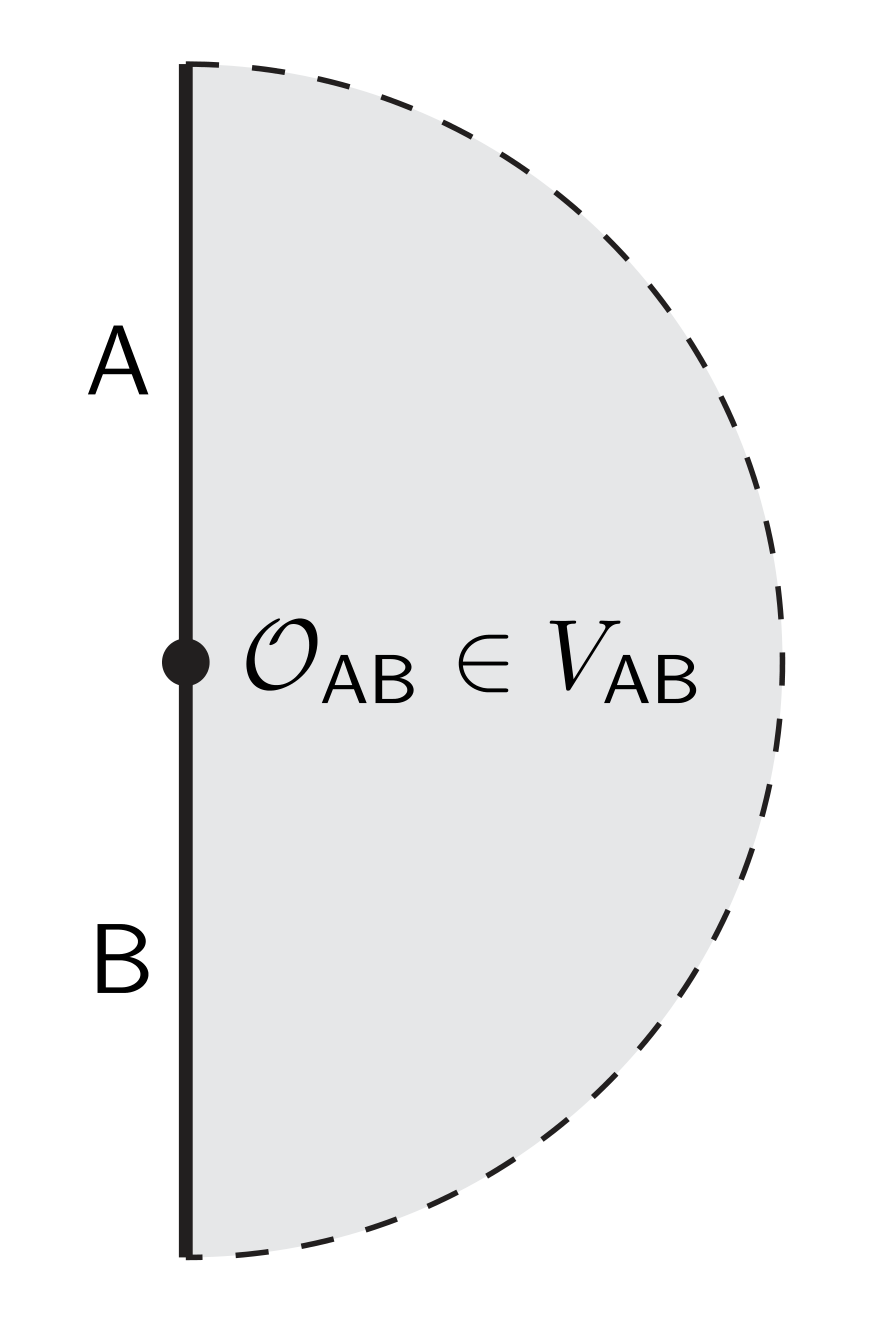
\includegraphics[width=0.34\linewidth]{fig1.png}
    \caption{膜范畴中的态射对应于位于边界两段接合处的边界变更局域算子。（原文 p.14，Figure 1）}
\end{figure}

\begin{figure}[htbp]
    \centering
    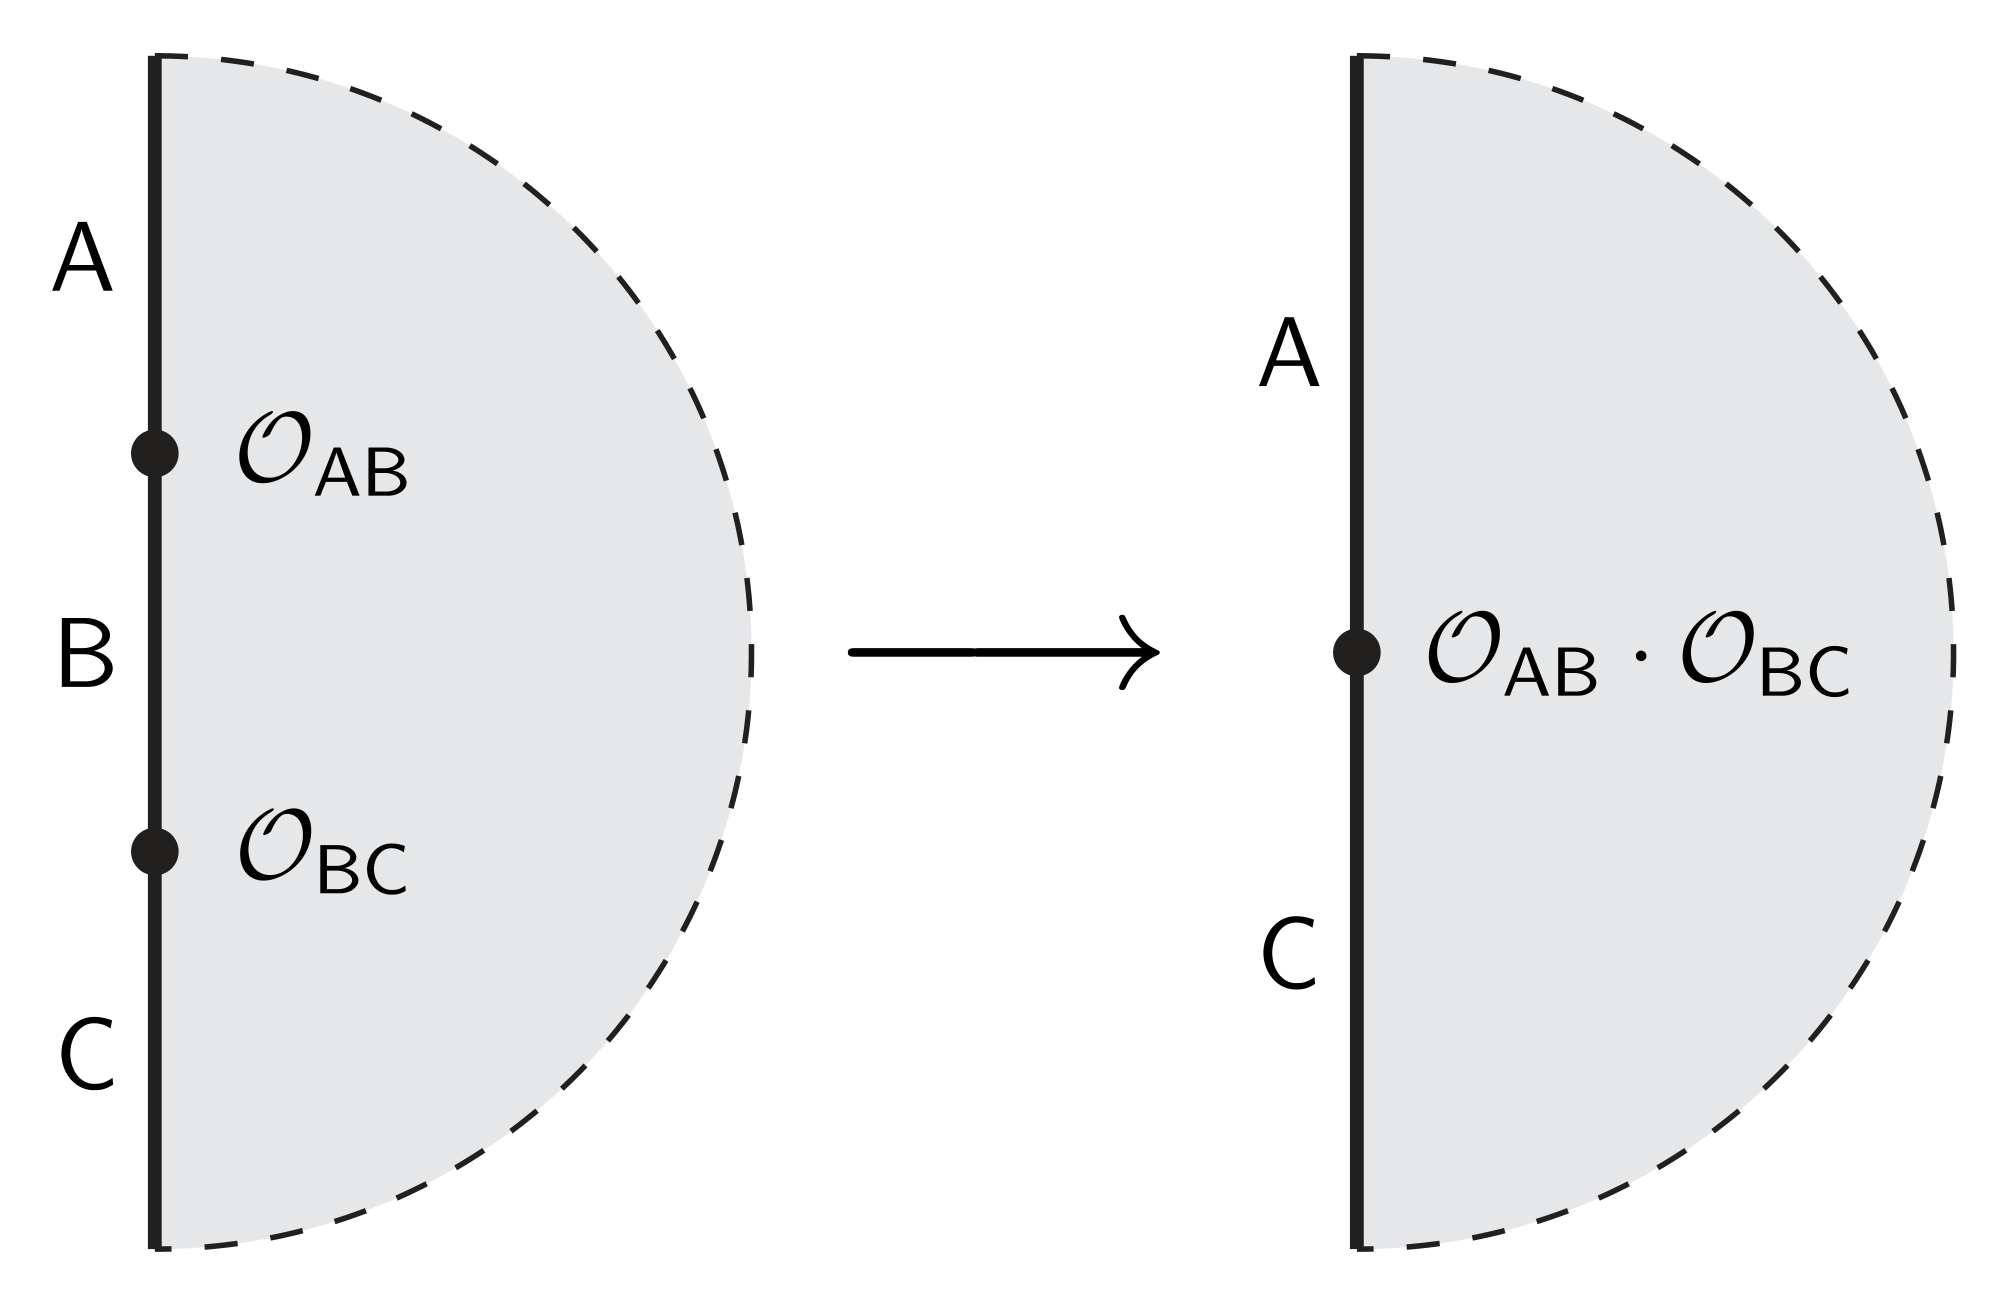
\includegraphics[width=0.62\linewidth]{fig2.png}
    \caption{态射的复合通过合并边界变更局域算子的插入点来实现；该运算记作 $\cdot$。（原文 p.14，Figure 2）}
\end{figure}

    % [Tutor Note: 见 p.13 与脚注 2。$\mathbb{V}_{\mathsf{A}\mathsf{B}}$ 与 $\mathbb{V}_{\mathsf{B}\mathsf{A}}$ 不同是"带向"的直接后果：把一段边界反向相当于取对偶，故通常可理解成 $\mathbb{V}_{\mathsf{B}\mathsf{A}}\simeq\mathbb{V}_{\mathsf{A}\mathsf{B}}^{*}$；只有额外给定非退化配对时两者才等同。这正是膜"范畴"的 Hom 不对称、必须使用带向配边范畴的原因。原文把这个空间的主字母排成黑板体、下标排成无衬线体（与正文边界条件 $\mathsf{A},\mathsf{B}$ 同族），故写作 $\mathbb{V}_{\mathsf{A}\mathsf{B}}$；译文保留原文的字体区别。]

    % [Tutor Note: 见 p.13 末与图 2。原文说"TFT 的性质保证复合是结合的（但不必交换）"，这实际上是说膜所构成的结构至少是一个范畴而不是群胚；若进一步把 $\mathbb{V}_{\mathsf{A}\mathsf{B}}$ 看成微分分次向量空间（例如在 A-模型中的情形），复合只在同伦意义下结合，得到的是 $A_{\infty}$-范畴。原文在"物理的严格性"层面把这些高阶结构省略了。]

现在也能理解为什么 $n$ 维 TFT 给紧致可定向的 $n-2$ 维流形 $L$ 指定一个范畴了。要点在于：把这样的 TFT 放在形如 $L\times\Sigma$ 的 $n$ 维流形上考虑（其中 $\Sigma$ 是一个可以带边界、不必紧致的定向 2-流形），可以把它视为 $\Sigma$ 上的 2 维 TFT，因而有膜的范畴。这个膜的范畴依赖于 $L$，它正是 $n$ 维 TFT 指定给 $L$ 的范畴。

再进一步，尝试理解为什么 $n$ 维 TFT 给紧致可定向的 $n-3$ 维流形 $K$ 指定一个 2-范畴。同样可以把这一 TFT 放在形如 $K\times W$ 的流形上考虑，其中 $W$ 是定向 3-流形（可以非紧，也可以带非空边界），并把它重新解释为 $W$ 上一个依赖于 $K$ 的 3 维 TFT。我们现在断言：任何 3d TFT 的边界条件集合都具有 2-范畴的结构；这个 2-范畴就是 $n$ 维 TFT 指定给 $K$ 的东西。

为了看清 3d TFT 中的边界条件为何构成 2-范畴，我们采用与 2d TFT 相同的想法：把 3-流形 $W$ 边界的某个连通分支分割成被闭合曲线隔开的若干区域，并在不同区域上施加不同的边界条件。给定两个边界条件 $\mathbb{X}$ 与 $\mathbb{Y}$，沿一条闭合曲线把它们"接合"的方式可能不止一种；按定义，$\mathbb{X}$ 与 $\mathbb{Y}$ 之间 1-态射的集合，就是沿余维 1 缺陷接合 $\mathbb{X}$ 与 $\mathbb{Y}$ 的不同方式之集合。边界上的余维 1 缺陷可以融合，由此得到 1-态射的复合（图 3）。

\begin{figure}[htbp]
    \centering
    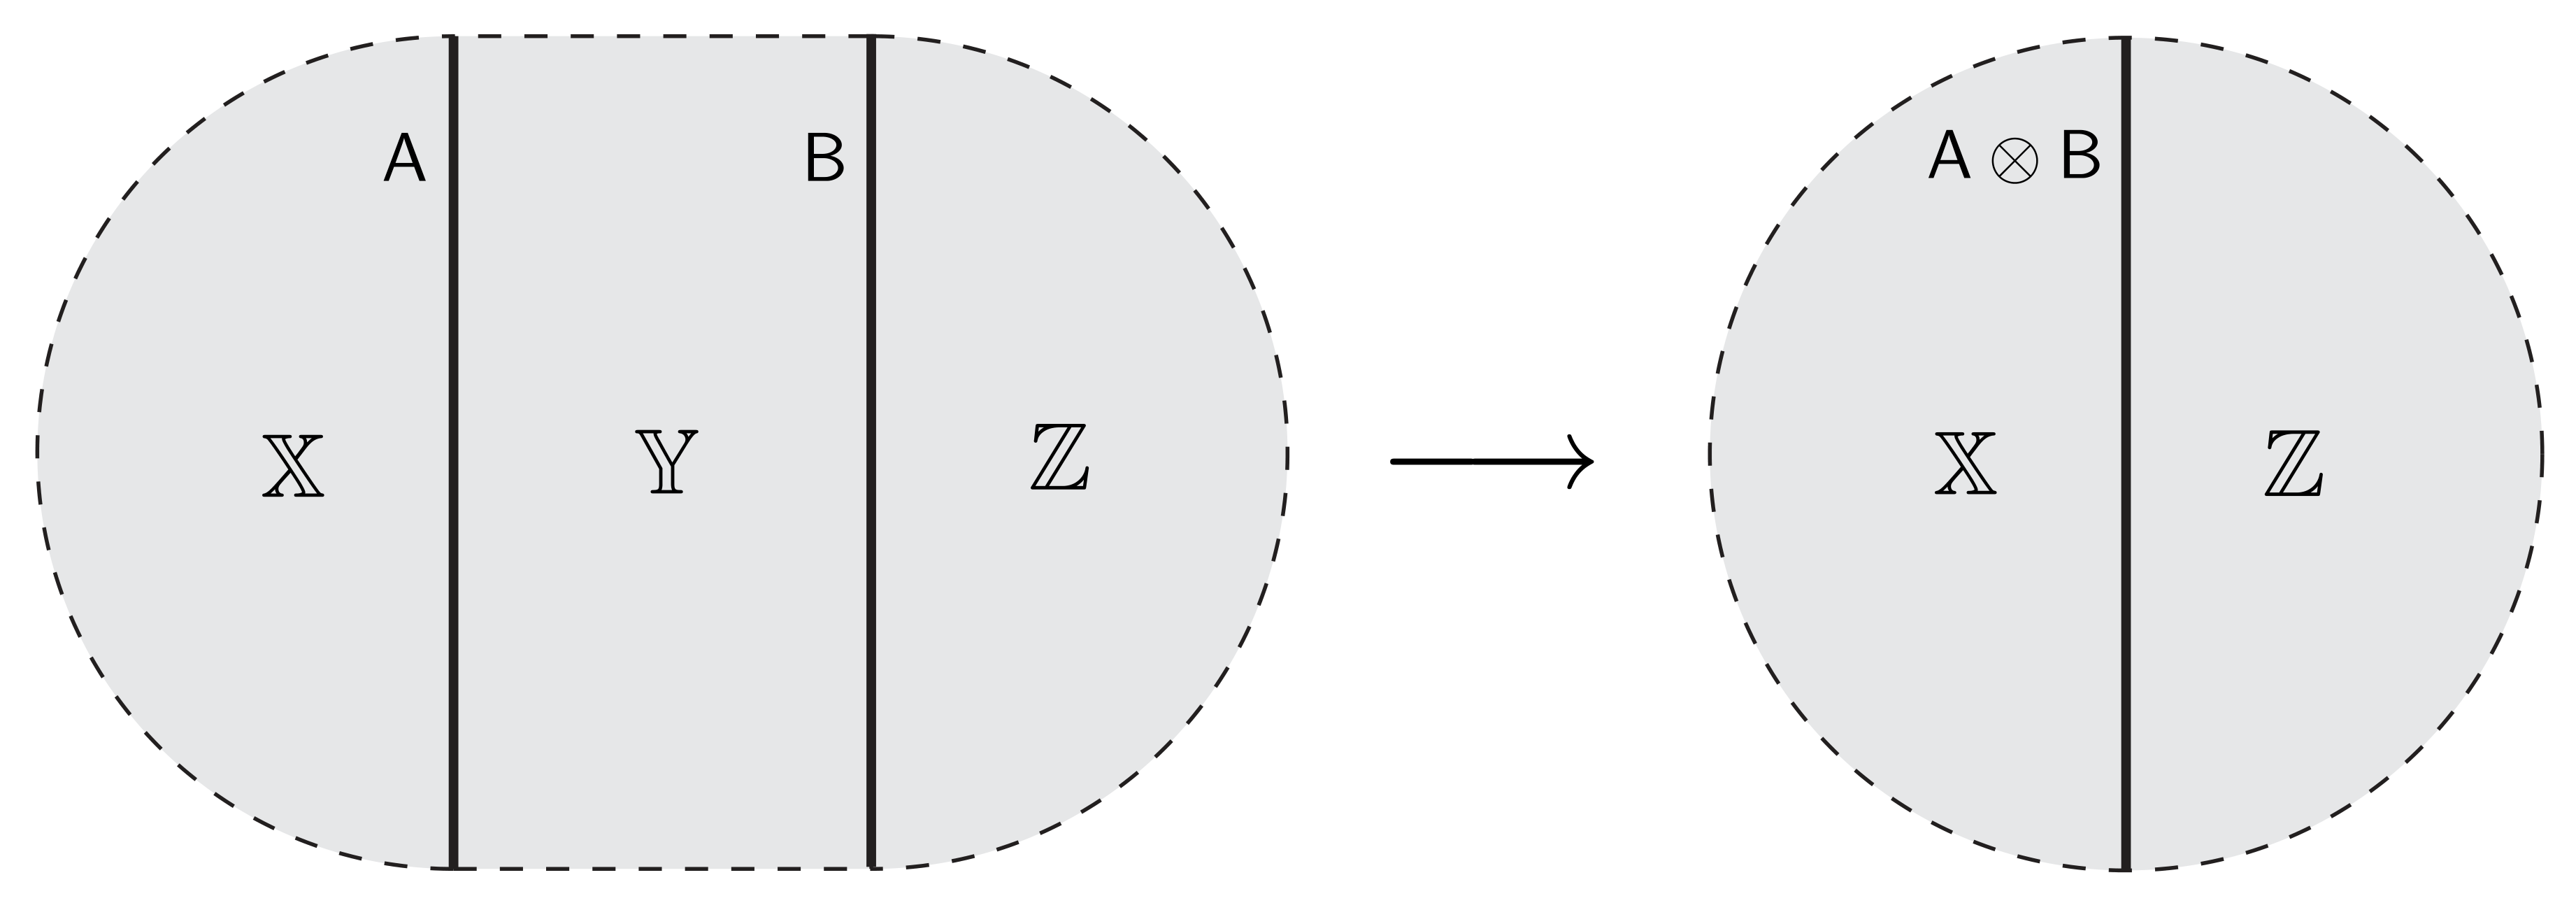
\includegraphics[width=0.86\linewidth]{fig3.png}
    \caption{2d TFT 的 2-范畴中的 1-态射对应于墙（wall），1-态射的复合对应于墙的融合；该运算记作 $\otimes$。（原文 p.15，Figure 3）}
\end{figure}

    % [Tutor Note: 见 p.15 与图 3 的图注。"2d TFT 的 2-范畴"这一说法容易被误读：这里的对象是 3d TFT 的边界条件，而每个这样的边界条件本身定义一个 2d TFT，所以该 2-范畴被称为"2d TFT 的 2-范畴"。1-态射是墙（边界上的余维 1 缺陷），2-态射则是墙上插入的局域算子。]

    $\partial W$ 上分隔边界条件 $\mathbb{X}$ 与 $\mathbb{Y}$ 所在区域的那条闭合曲线可以再分割成若干线段，并在不同线段上赋予不同的余维 1 缺陷。不同线段相接的那些点是边界上的余维 2 缺陷；在余维 2 缺陷处接合余维 1 缺陷 $\mathsf{A}$ 与 $\mathsf{B}$ 的不同方式，就是边界条件 2-范畴的 2-态射。基本的物理原理是：2-态射的集合具有（分次）向量空间的结构。我们可以把余维 1 缺陷连同余维 2 缺陷一起融合；由此得到 2-态射的"水平"复合（图 4）。

\begin{figure}[htbp]
    \centering
    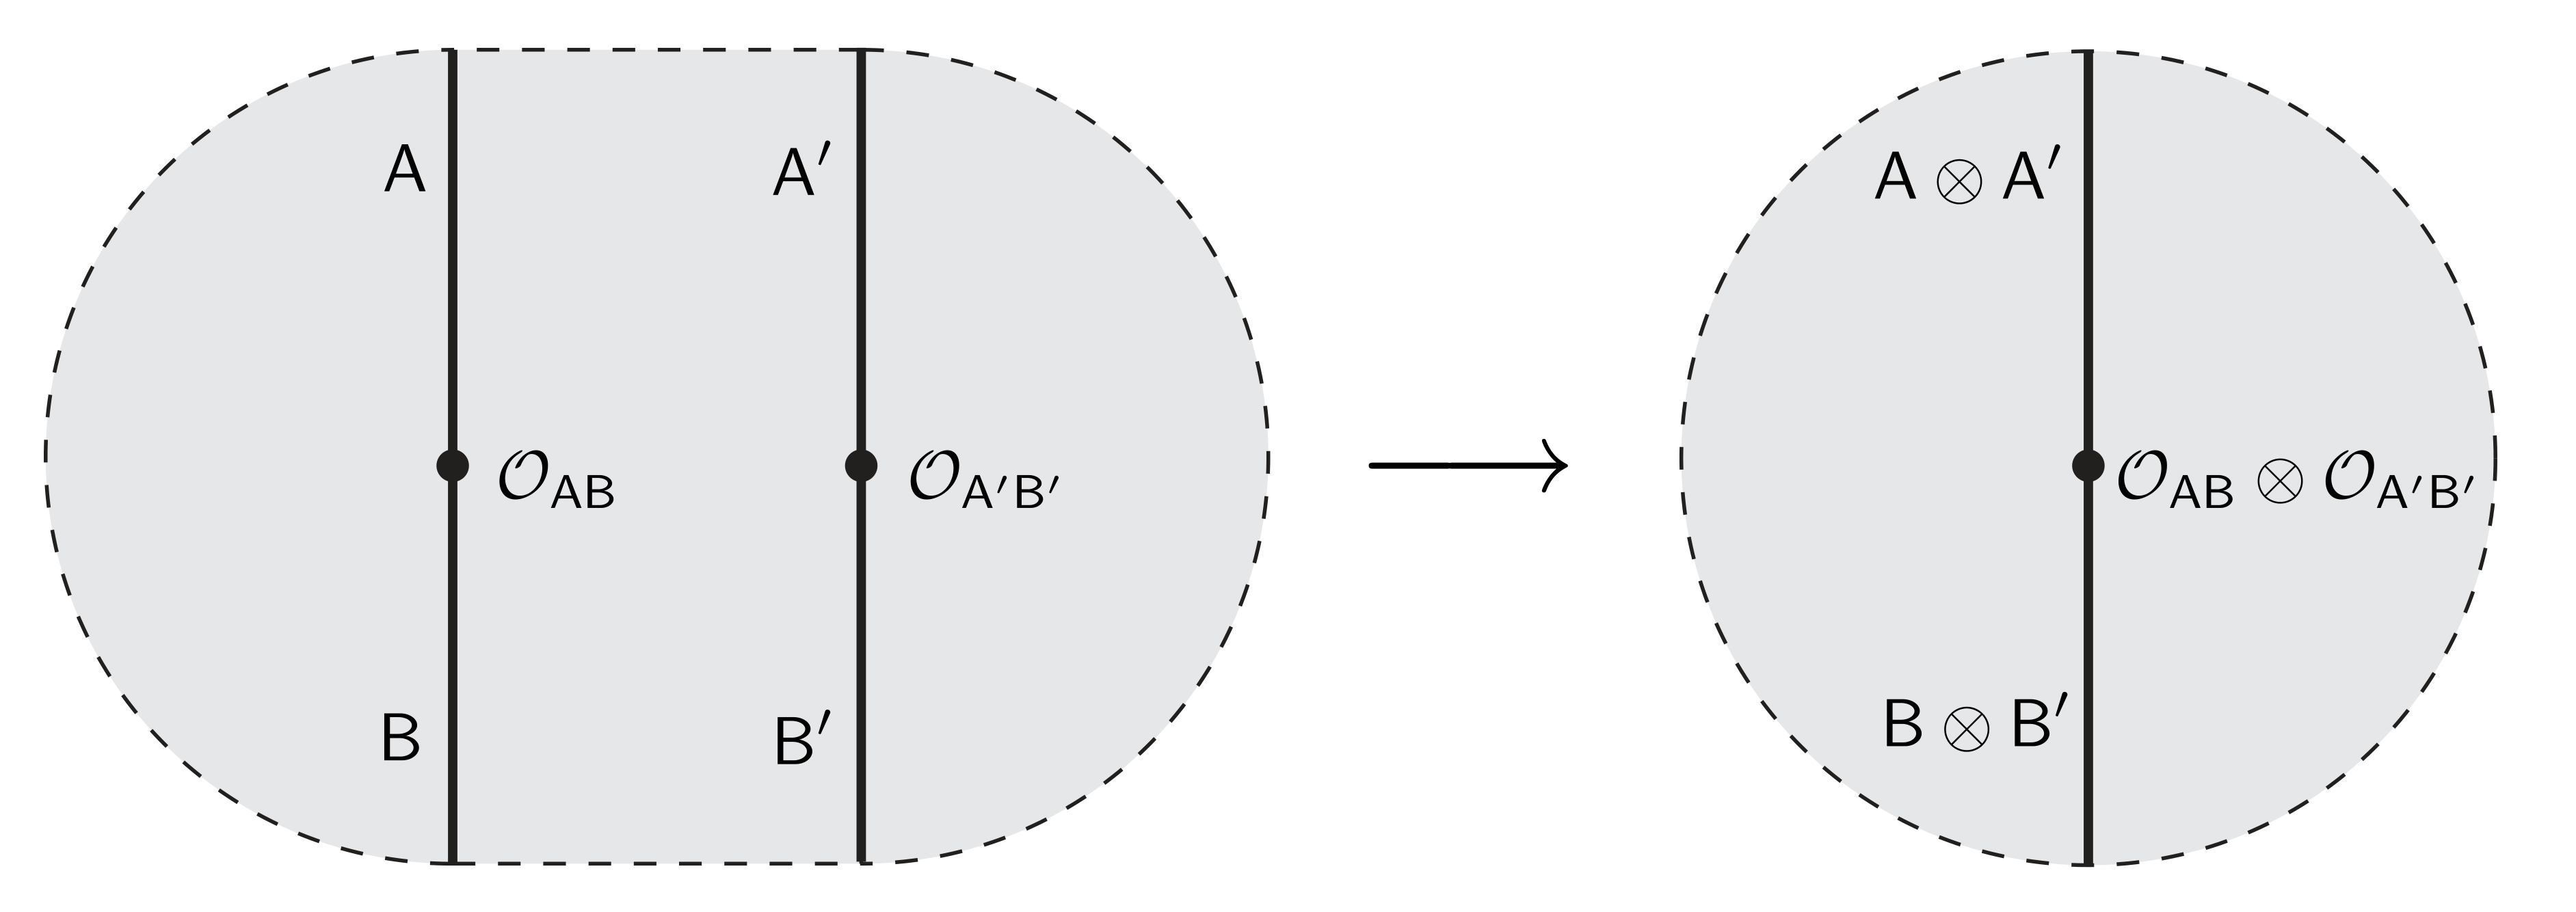
\includegraphics[width=0.98\linewidth]{fig4.png}
    \caption{2d TFT 的 2-范畴中 2-态射的复合，通过融合其插入所在的那堵墙来实现；相应运算记作 $\otimes$。（原文 p.16，Figure 4）}
\end{figure}

还存在 2-态射的"垂直"复合，它来自把位于同一余维 1 缺陷上、被分割成若干线段的余维 2 缺陷融合起来。固定一对边界条件 $\mathbb{X}$ 与 $\mathbb{Y}$，它们之间的所有余维 1 缺陷连同其上的所有余维 2 缺陷构成一个范畴。给定 3d TFT 的所有边界条件连同所有余维 1、余维 2 缺陷，则构成一个 2-范畴。这就是 3d TFT 指定给一个点的 2-范畴。

    % [Tutor Note: 见 p.15 末段。2-态射有"水平"与"垂直"两种复合：水平复合是把墙与墙上的插入点一起融合（图 4），垂直复合是在同一条被分割的墙上把插入点融合。2-范畴公理还要求这两者满足交换律（interchange law）；原文没有明说，但图 4 的构造正是为了让这条公理成立。]

\section{约化到二维}

\begin{keypoints}
    \item \textbf{物理图像：}4d TFT 给点一个（目前尚未被理解的）3-范畴、给圆一个 2-范畴（其对象为面算子）、给紧致定向曲面 $C$ 一个普通范畴；讲义只研究最后一个。
    \item \textbf{数学工具：}把 $C\times\Sigma$ 上的 4d TFT 看作 $\Sigma$ 上依赖于 $C$ 的 2d TFT，再令 $\operatorname{vol}(C)\to0$ 作 Kaluza--Klein 式约化，得到以 Hitchin 模空间 $\mathcal{M}_{H}(G,C)$ 为目标的拓扑 $\sigma$-模型。
    \item \textbf{关键结论：}$\mathcal{M}_{H}(G,C)$ 是非紧超凯勒流形，实维数 $4(g-1)\dim G$，带奇点；其上由 $\mathbb{P}^{1}$ 参数化的一族复结构给出一族 B-模型，相应的凯勒形式给出一族 A-模型。
    \item \textbf{关键机制：}一般 A-模型或 B-模型依赖 $C$ 的复结构，故 4d 约化对应的是 $\mathbb{P}^{1}\times\mathbb{P}^{1}$ 族中不依赖 $C$ 的一维子族 $w_{+}=-t$、$w_{-}=t^{-1}$：$t=i$ 为 B-模型（复结构 $J$，$\mathcal{M}_{flat}$），$t=1$ 为 A-模型（辛形式 $4\pi\omega_{K}/e^{2}$），$t=0$ 为 $\mathcal{M}_{Higgs}$ 的 A-模型。
\end{keypoints}

我们的主要研究对象是一个 4d TFT（更确切地说，是由 $t\in\mathbb{CP}^{1}$ 和规范群 $G$ 的选择所参数化的一族 4d TFT）。这样的 TFT 给一个点指定一个 3-范畴，给一个圆指定一个 2-范畴，给紧致可定向的 2-流形 $C$ 指定一个普通范畴。可以说，指定给点的 3-范畴（即边界条件的 3-范畴）目前尚未被理解，尽管 D.~Gaiotto 与 E.~Witten [23, 24] 已经构造出其中的一些对象。依附于圆的 2-范畴的对象在物理文献中称为面算子（surface operator）；对它们的研究由 S.~Gukov 与 E.~Witten [7, 8, 9] 开创，面算子集合上的 2-范畴结构已在 [25] 中讨论过。在本次讲义中，我们只研究依附于紧致可定向 2-流形 $C$ 的范畴。仿照 [6]，我们假定 $C$ 的亏格 $g>1$。\footnote{$g=0$ 的情形已在 [25] 中研究。}于是我们考虑形如 $X=C\times\Sigma$ 的 4-流形上的 4d TFT（其中 $\Sigma$ 可以非紧，也可以带非空边界），把它视为 $\Sigma$ 上一个依赖于 $C$ 的 2d TFT，并研究它的膜范畴。

    % [Tutor Note: 见 p.16。4d TFT 给点指定 3-范畴，这是"完全扩展"猜想中最难的一层，原文明确说它尚未被理解；Gaiotto--Witten [23, 24] 构造的是其中一些对象（边界条件）。给圆指定 2-范畴，其对象即"面算子"，也就是 4d 中的余维 2 缺陷。脚注 3 提到的 $g=0$ 情形见 [25]。]

拓扑关联函数不依赖于 $C$ 与 $\Sigma$ 的体积。然而，为了利用局域化，考虑让 $C$ 的体积趋于零的极限是方便的。按照 Kaluza--Klein 约化的精神，我们预期在这个极限下 4 维理论等价于 $\Sigma$ 上的一个 2 维理论。在未扭曲的理论中，这一等价只在 $\operatorname{vol}(C)\to0$ 的极限下成立；而在扭曲理论中，该等价对任何体积都成立。

    % [Tutor Note: 见 p.16 末至 p.17 首。这里的"约化"是 Kaluza--Klein 式的：$C$ 缩成一点，4d 理论化为 $\Sigma$ 上的 2d 理论，其目标空间是 $C$ 上的真空模空间。扭曲理论的优越性在于超对称对任何体积都保持（拓扑扭曲后能量--动量张量是 $Q$-恰当的），所以等价性不限于 $\operatorname{vol}(C)\to0$；未扭曲理论则只在极限下成立。]

猜测 $\Sigma$ 上的有效场论并不困难。先考虑 $\Sigma=\mathbb{R}^{2}$ 的情形，并要求场组态不依赖于 $\Sigma$ 上的坐标、且能量为零。可以证明，一般的这种组态满足 $\sigma=0$，而 $\phi$ 与 $A$ 是从 $C$ 拉回的量，并满足
\[
    F-\phi\wedge\phi=0,\qquad D\phi=0,\qquad D\star\phi=0.
\]
这里所有的量以及 Hodge 星算子都指 $C$ 上的对象而言。这些方程称为 Hitchin 方程 [19]，其解模去规范变换所得的空间称为 Hitchin 模空间 $\mathcal{M}_{H}(G,C)$。空间 $\mathcal{M}_{H}(G,C)$ 是一个非紧流形，维数为 $4(g-1)\dim G$，并且带有奇点。\footnote{我们假定 $g>1$，正是为了保证 $\mathcal{M}_{H}(G,C)$ 的虚维数为正。}从物理观点看，$\mathcal{M}_{H}(G,C)$ 是 $C\times\mathbb{R}^{2}$ 上扭曲的 $\mathcal{N}=4$ SYM 的经典真空空间。

    % [Tutor Note: 见 p.17 的 Hitchin 方程。三个方程的实/复性质是本节最易错处：(i) $F-\phi\wedge\phi=0$ 与 (ii) $D\phi=0$ 都是 $C$ 上的实方程，且不含 $C$ 的度规；(iii) $D\star\phi=0$ 含有 Hodge 星，因而依赖 $C$ 的度规。这里的 $\star$ 是二维曲面 $C$ 上的 Hodge 星，它把 1-形式映回 1-形式（在二维黎曼流形上 $\star^{2}=1$）；原文特意声明"所有的量以及 Hodge 星算子都指 $C$ 上的对象"，切勿误用 4 维时空的 Hodge 星。另注意第三个方程是 $D\star\phi=0$ 而不是 $D\phi=0$。]

在扭曲理论中，只有能量小到可以忽略的组态才有贡献。在 $\operatorname{vol}(C)\to0$ 的极限下，这类组态将由从 $\Sigma$ 到 $\mathcal{M}_{H}(G,C)$ 的缓变映射来代表。因此我们预期 $\Sigma$ 上的有效场论是以 $\mathcal{M}_{H}(G,C)$ 为目标的拓扑 $\sigma$-模型。

在更精确地辨认这个拓扑 $\sigma$-模型之前，先指出 $\mathcal{M}_{H}(G,C)$ 的奇点来源于那些在规范变换的某个子群下不变的 Hitchin 方程解。在这样的经典真空附近，由于存在未破缺的规范对称性，有效场论并不等价于一个 $\sigma$-模型；事实上，用纯 2 维的语言很难描述这类真空附近的物理。我们将通过在 $\Sigma$ 的边界上施加适当条件、确保远离这些危险点，来回避这一困难。

拓扑 $\sigma$-模型最熟悉的例子是与 Calabi--Yau 流形 $M$ 相联系的 A-模型与 B-模型 [26]。两个模型都通过对以 $M$ 为目标的超对称 $\sigma$-模型作扭曲而得到。A-模型的路径积分局域化到从 $\Sigma$ 到 $M$ 的全纯映射上，并计算 $M$ 的 Gromov--Witten 不变量；B-模型的路径积分局域化到 $M$ 的常映射上，并可以在数学上用把 $M$ 看作复流形时的形变理论来解释 [27]。两个模型都是拓扑场论（TFT），即其关联函数不依赖于 $\Sigma$ 上的度规。此外，A-模型依赖于 $M$ 的辛结构而不依赖于其复结构，B-模型则依赖于 $M$ 的复结构而不依赖于其辛结构。

如上所述，我们预期这一族 4d TFT 在形如 $\Sigma\times C$ 的 4-流形上考虑时，等价于一族以 $\mathcal{M}_{H}(G,C)$ 为目标的拓扑 $\sigma$-模型。为了把这族模型与通常的 A、B-模型联系起来，注意 $\mathcal{M}_{H}(G,C)$ 是一个（非紧的）超凯勒流形。也就是说，它具有 $\mathbb{P}^{1}$ 那样多的、与某个度规相容的复结构。该度规的形式为
\[
    ds^{2}=\frac{1}{e^{2}}\int_{C}\operatorname{Tr}\left(\delta A\wedge\star\delta A+\delta\phi\wedge\star\delta\phi\right),
\]
其中 $(\delta A,\delta\phi)$ 是线性化 Hitchin 方程的一个解，代表 $\mathcal{M}_{H}(G,C)$ 的一个切向量。\footnote{我们采用的度规整体归一化，从规范理论的观点看是自然的。}若用一个参数 $w\in\mathbb{C}\cup\{\infty\}$ 来参数化这个复结构球，则全纯微分的基为
\[
    \delta A_{\bar z}-w\,\delta\phi_{\bar z},\qquad
    \delta A_{z}+w^{-1}\delta\phi_{z}.
\]
改变 $w$ 就得到一族以 $\mathcal{M}_{H}(G,C)$ 为目标的 B-模型。类似地，由于对每个 $w$ 都有 $\mathcal{M}_{H}(G,C)$ 上相应的凯勒形式，改变 $w$ 又得到一族以 $\mathcal{M}_{H}(G,C)$ 为目标的 A-模型。然而，由扭曲的 $\mathcal{N}=4$ SYM 得到的这族拓扑 $\sigma$-模型与上述两族中的任何一族都不重合。原因在于：以 $\mathcal{M}_{H}(G,C)$ 为目标的一般 A-模型或 B-模型依赖于 $C$ 的复结构，因而不能来自 $\Sigma\times C$ 上的 TFT。

    % [Tutor Note: 见 p.18。$\mathcal{M}_{H}(G,C)$ 是超凯勒流形，其上的复结构构成一整个 $\mathbb{P}^{1}$。原文的 $ds^{2}$（脚注 5 说明其归一化"从规范理论的观点看是自然的"）与下文各凯勒形式的归一化必须配套使用：$1/e^{2}$ 中的 $e$ 是 4d 规范耦合常数，所以这里的"度规"实际上是一族依赖于 $e$ 的度规。]

    % [Tutor Note: 见 p.18 的全纯微分基。$\delta A_{\bar z}-w\,\delta\phi_{\bar z}$ 与 $\delta A_{z}+w^{-1}\delta\phi_{z}$ 是复结构 $w$ 下全纯微分（即 $(1,0)$-形式）的基。注意两处系数不对称：作用在 $\bar z$ 分量上的是 $-w$，作用在 $z$ 分量上的是 $w^{-1}$，且后者是 $w$ 的逆而不是 $w$；抄写时若把 $w^{-1}$ 写成 $w$ 或丢掉负号，给出的就是 $\mathbb{P}^{1}$ 上另一个参数值对应的复结构，下文 $w_{+}=-t$、$w_{-}=t^{-1}$ 的判据也会随之改变。]

正如 [6] 所解释的，只要回想超凯勒流形 $M$ 上除通常的 A-扭曲与 B-扭曲之外还有别的扭曲，这个疑难就解决了。一般地，扭曲一个超对称 $\sigma$-模型需要在目标上选取两个复结构。如果给定 $M$ 上的一个凯勒结构，可以取这两个复结构相同（B-扭曲）或相反（A-扭曲）。但对超凯勒流形而言，存在整整一个球的复结构，独立地改变这两个复结构就得到 $\mathbb{P}^{1}\times\mathbb{P}^{1}$ 那样多的 2d TFT。它们被称为广义拓扑 $\sigma$-模型，因为其关联函数依赖于目标 $M$ 上的广义复结构 [28, 29]。广义复结构的概念由 N.~Hitchin [30] 引入，复结构与辛结构都是它的特例。

结果表明，对于 $M=\mathcal{M}_{H}(G,C)$，在这个 2-参数族的拓扑 $\sigma$-模型中存在一个 1-参数子族，它不依赖于 $C$ 的复结构或凯勒形式。正是这个子族作为扭曲的 $\mathcal{N}=4$ SYM 理论的约化而出现。具体地说，$\mathcal{M}_{H}(G,C)$ 上的两个复结构由
\[
    w_{+}=-t,\qquad w_{-}=t^{-1}
\]
给出。注意，当且仅当 $w_{+}=w_{-}$，即 $t=\pm i$ 时，得到的是 B-模型；当且仅当 $t$ 为实数时，得到的是 A-模型；$t$ 的其余取值都对应广义拓扑 $\sigma$-模型。

    % [Tutor Note: 见 p.18 "one gets a B-model if and only if $w_{+}=w_{-}$"。这是本节最易混的约定：判据是"两个扭曲复结构相同 $\Leftrightarrow$ B-模型、相反 $\Leftrightarrow$ A-模型"，而不是 $t$ 的虚实本身；只是在 $w_{+}=-t$、$w_{-}=t^{-1}$ 这个一维子族里，两者恰好等价（$t=\pm i$ 给 B-模型，$t$ 实给 A-模型）。尤其注意：$t=i$ 给出的是 B-模型（复结构 $J$，即稳定平坦 $G_{\mathbb{C}}$ 联络的模空间），$t=1$ 给出的才是 A-模型（辛形式 $4\pi\omega_{K}/e^{2}$，复结构 $K$）；初学者常把它误记成"$t=i$ 是 A-模型"。另外不要把这里的 $t$ 与规范耦合 $\tau$（其定义见前文）混为一谈：$t$ 是 $\mathbb{CP}^{1}$ 上的扭曲参数，前文已说明 MO 对偶把 $t$ 乘以相位 $|\tau|/\tau$，二者只在特定对应下才相联系。]

幸运的是，为了理解几何朗兰兹对偶，我们主要需要 $t=i$ 与 $t=1$ 这两个特殊情形。$t=i$ 对应于复结构 $J$ 的 B-模型，$J$ 由 $\mathcal{M}_{H}(G,C)$ 上的复坐标
\[
    A_{z}+i\phi_{z},\qquad A_{\bar z}+i\phi_{\bar z}
\]
定义。它们正是 $C$ 上复联络 $\mathcal{A}=A+i\phi$ 的分量。用这个复联络表示时，三个 Hitchin 方程中的两个等价于
\[
    \mathcal{F}=\mathrm{d}\mathcal{A}+\mathcal{A}^{2}=0.
\]
这个方程在复化规范变换下不变；第三个方程 $D\star\phi=0$ 则只在 $G$ 的规范变换下不变。按 S.~Donaldson [31] 的定理，可以丢掉这个方程，代价是把规范群从 $G$ 放大到 $G_{\mathbb{C}}$。（更精确地说，还须把方程 $\mathcal{F}=0$ 的某些半稳定解等同起来。）这与四维中的情形类似。于是在复结构 $J$ 下，模空间 $\mathcal{M}_{H}(G,C)$ 可以等同于 $C$ 上稳定平坦 $G_{\mathbb{C}}$ 联络的模空间 $\mathcal{M}_{flat}(G,C)$。显然 $J$ 不依赖于 $C$ 上的复结构，这就意味着 $t=i$ 时的 B-模型也不依赖于它。

    % [Tutor Note: 见 p.19 "two out of three Hitchin equations are equivalent to $\mathcal{F}=0$"。要会自己验证：把 $\mathcal{A}=A+i\phi$ 代入，用 $A\wedge\phi+\phi\wedge A=[A,\phi]$，得 $\mathcal{F}=\mathrm{d}\mathcal{A}+\mathcal{A}\wedge\mathcal{A}=(F-\phi\wedge\phi)+i\,D\phi$；故 $\mathcal{F}=0$ 的实部、虚部分别恰是 $F-\phi\wedge\phi=0$ 与 $D\phi=0$，剩下的正是含度规的 $D\star\phi=0$。这也解释了为什么丢掉第三个方程只需付"复化规范群"的代价。]

    % [Tutor Note: 见 p.19 "By a theorem of S. Donaldson [31]"。这里省掉的逻辑是 Hitchin--Kobayashi 对应（Donaldson 1987，Simpson 推广）：$C$ 上（半）稳定的希格斯丛，其 $G_{\mathbb{C}}$-轨道中存在满足完整 Hitchin 方程（含 $D\star\phi=0$）的联络；反过来，丢掉 $D\star\phi=0$ 后 $G_{\mathbb{C}}$ 作用下的解空间必须用几何不变量理论（GIT）作商、只保留半稳定解，才能与原来的 Hitchin 模空间一致。原文说"这与四维中的情形类似"，指的是四维瞬子模空间与稳定全纯丛的对应。]

    % [Tutor Note: 见 p.17 脚注 4 与 p.19 维数公式。$\mathcal{M}_{H}(G,C)$ 的实维数是 $4(g-1)\dim G$，等价地复维数是 $2(g-1)\dim G$（与 $g>1$ 时 $\dim_{\mathbb{C}}\operatorname{Bun}_{G}=(g-1)\dim G$ 及 $T^{*}\operatorname{Bun}_{G}$ 的维数相符）。$g>1$ 正是使这个"虚维数"为正的条件；$g=1$ 时维数为零、$g=0$ 时为负，故原文用脚注 4 明确点出这一假设的动机。]

    $t=1$ 对应于一个 A-模型，其辛结构为 $\omega=4\pi\omega_{K}/e^{2}$，其中
\[
    \omega_{K}=-\frac{1}{2\pi}\int_{C}\operatorname{Tr}\delta\phi\wedge\delta A.
\]
它是 $\mathcal{M}_{H}(G,C)$ 上某个复结构 $K$ 的凯勒形式。注意 $\omega_{K}$ 是恰当的，且不依赖于 $C$ 上的复结构。

    % [Tutor Note: 见 p.18--p.19 的 $\omega_{K}$ 与 $\omega_{I}$。两者归一化不同，最容易抄错：$\omega_{K}=-\frac{1}{2\pi}\int_{C}\operatorname{Tr}\delta\phi\wedge\delta A$ 只有一项、系数是 $1/2\pi$；而 $\omega_{I}=\frac{1}{4\pi}\int_{C}\operatorname{Tr}(\delta A\wedge\delta A-\delta\phi\wedge\delta\phi)$ 有两项、系数是 $1/4\pi$，且第二项带负号。物理辛形式为 $\omega=4\pi\omega_{K}/e^{2}$，代入定义可作一致性检查：$\omega=-\frac{2}{e^{2}}\int_{C}\operatorname{Tr}\delta\phi\wedge\delta A$，$4\pi$ 与 $1/2\pi$ 恰好相消。$\omega_{K}$ 与 $\omega_{I}$ 是超凯勒三元组 $(\omega_{I},\omega_{J},\omega_{K})$ 中的两个，它们对同一度规两两相容。]

    $\mathcal{M}_{H}(G,C)$ 上还有一个复结构 $I=JK$。在后面讨论 $\mathcal{M}_{H}(G,C)$ 的同调镜像对称（Homological Mirror Symmetry）时，它会出现。在这个复结构下，$\mathcal{M}_{H}(G,C)$ 可以等同于稳定全纯希格斯丛的模空间。回忆一下：$C$ 上（规范群为 $G$ 的）（全纯）希格斯丛，是一个 $C$ 上的全纯 $G$-丛 $E$，连同 $\operatorname{ad}(E)$ 的一个全纯截面 $\varphi$。在一维复维数下，任何主 $G$-丛都可以看作全纯丛，而 Hitchin 方程蕴涵 $\varphi=\phi^{1,0}$ 满足
\[
    \bar\partial\varphi=0.
\]
这给出从 $\mathcal{M}_{H}(G,C)$ 到希格斯丛的规范等价类集合的一个映射。若我们只限于稳定或半稳定的希格斯丛，并对半稳定的那些施加适当的等价关系，这个映射就变成一一的。由此得到 $\mathcal{M}_{H}(G,C)$ 与 $\mathcal{M}_{Higgs}(G,C)$ 之间的同构。

    % [Tutor Note: 见 p.19 "a holomorphic section $\varphi$ of $\operatorname{ad}(E)$"。严格地说，希格斯场应是 $\operatorname{ad}(E)\otimes K_{C}$ 的全纯截面（$K_{C}$ 为 $C$ 的典范线丛），即 $\varphi=\phi^{1,0}$ 是取值为 $(1,0)$-形式的截面；原文写作"$\operatorname{ad}(E)$ 的截面"省略了 $K_{C}$，属于行文简略。译文保留原文措辞，请读者按 $\operatorname{ad}(E)\otimes K_{C}$ 理解。另注意原文区分两种字形：Hitchin 方程中的 1-形式记作 $\phi$，而全纯希格斯场记作 $\varphi=\phi^{1,0}$，正文中不可混用。]

显然，与 $J$ 不同，复结构 $I$ 确实依赖于 $C$ 上复结构的选择。因此，稳定希格斯丛模空间的 B-模型不能作为某个 4d TFT 的约化而得到。\footnote{它可以作为 $\Sigma\times C$ 上一种"全纯-拓扑"规范理论的约化而得到 [32]。}另一方面，$\mathcal{M}_{Higgs}(G,C)$ 的 A-模型不依赖于 $C$ 上复结构的选择，因为凯勒形式 $\omega_{I}$ 由
\[
    \omega_{I}=\frac{1}{4\pi}\int_{C}\operatorname{Tr}\left(\delta A\wedge\delta A-\delta\phi\wedge\delta\phi\right)
\]
给出。事实上，$\mathcal{M}_{Higgs}(G,C)$ 的 A-模型是通过令 $t=0$ 得到的。这一约化到 2d 的特殊情形最早在 [33] 中讨论过。

    % [Tutor Note: 见 p.19 末。$t=0$ 时 $w_{+}=0$、$w_{-}=\infty$，两个复结构"相反"，故给 A-模型；它以 $\mathcal{M}_{Higgs}(G,C)$ 为目标，且 $\omega_{I}$ 的表达式只含 $\delta A$、$\delta\phi$ 而不含 $C$ 的复结构，所以这个 A-模型与 $C$ 的复结构无关——这正是它能作为 4d TFT 约化出现的原因，与 $I$ 本身依赖 $C$ 的复结构并不矛盾。]

% ==================================================================
%  片段 s04.tex
% ==================================================================
\section{Hitchin 模空间的镜像对称}

\begin{keypoints}
    \item \textbf{物理图像：}当 $\theta=0$ 时，MO 对偶把规范群 ${}^{L}G$、$t=i$ 的扭曲 $\mathcal{N}=4$ 超对称杨–米尔斯理论与规范群 $G$、$t=1$ 的相应理论等同，故 $\mathcal{M}_{flat}({}^{L}G,C)$ 上的 B-模型与 $(\mathcal{M}_{H}(G,C),\omega_{K})$ 上的 A-模型等价，二者构成镜像对。
    \item \textbf{数学工具：}Frobenius 流形同构只反映 Gromov–Witten 不变量与复结构形变；更强也更本质的表述是同调镜像对称，即凝聚层导出范畴与 A-膜范畴的等价。
    \item \textbf{关键结论：}Hitchin 纤维化的底为 $\bigoplus_{n=2}^{N}H^{0}(C,K_{C}^{n})$，其纤维在复结构 $J$、$K$ 中拉格朗日，恰是 SYZ 纤维化；$\Omega_{I}=\omega_{J}+i\omega_{K}$ 使其成为复可积系统。
    \item \textbf{证明策略：}用 $\mathcal{P}_{n}$ 的真空期望值参数化 $X=\mathbb{R}^{4}$ 上的真空模空间，MO 对偶必须等同两侧的真空模空间，由此把 Hitchin 纤维化与 SYZ 纤维化对齐；光滑点的结构层之镜像即对偶纤维上的 A-膜。
    \item \textbf{技术限制：}$\mathcal{M}_{H}(G,C)$ 的分支由 $\pi_{1}(G)$ 标记，故上述论证需 $G$ 与 ${}^{L}G$ 均单连通（紧单李群中仅 $\mathrm{E}_{8}$、$\mathrm{F}_{4}$、$\mathrm{G}_{2}$）；一般情形须用取值于 $H^{2}(C,Z(G))=Z(G)$ 的平坦 B-场与 $\pi_{1}({}^{L}G)$ 的对应来补偿。
\end{keypoints}

现在我们可以推出 MO 对偶对以 $\mathcal{M}_{H}(G,C)$ 为目标的拓扑 $\sigma$-模型的推论了。当 $\theta=0$ 时，MO 对偶把规范群为 ${}^{L}G$、$t=i$ 的扭曲 $\mathcal{N}=4$ 超对称杨–米尔斯理论与规范群为 $G$、$t=1$ 的类似理论等同起来。因此，以 $\mathcal{M}_{flat}({}^{L}G,C)$ 为目标的 B-模型与以 $(\mathcal{M}(G,C),\omega_{K})$ 为目标的 A-模型是同构的。

% [Tutor Note: p.20 首段把 A-模型的目标写成 (\mathcal{M}(G,C),\omega_K)，但本段开头说的是“以 \mathcal{M}_H(G,C) 为目标的拓扑 sigma-模型”，p.22 的总结段亦写作 \mathcal{M}_H(G,C)（配以恰当辛形式 \omega_K）。故此处应为 \mathcal{M}_H(G,C)，原文疑漏写下标 H；译文保留原样以便与原文对照。]

% [Tutor Note: p.20 关于 t 参数的对应原文未加推导：0.6 节已说明 t=i 给出 B-模型、t=1 给出辛形式 \omega=4\pi\omega_K/e^2 的 A-模型，而 MO 对偶（\theta=0）在拓扑层面把这两个模型配对；t 在 S-对偶下的具体变换约定见 [6] 第 5--6 节。]

每当我们有两个 Calabi–Yau 流形 $M$ 与 $M'$，使得 $M$ 的 A-模型等价于 $M'$ 的 B-模型时，就说 $M$ 与 $M'$ 构成一对镜像对（mirror pair）。于是 MO 对偶蕴含 $\mathcal{M}_{flat}({}^{L}G,C)$ 与 $\mathcal{M}_{H}(G,C)$（配以辛结构 $\omega_{K}$）是一对镜像对。这一镜像对称最早在 [34] 中提出。

对这一陈述最显然的数学解释，是给出与 $(\mathcal{M}_{H}(G,C),\omega_{K})$ 的 A-模型及 $\mathcal{M}_{flat}({}^{L}G,C)$ 的 B-模型相关联的两个 Frobenius 流形之间的同构。前者编码 $\mathcal{M}_{H}(G,C)$ 的 Gromov–Witten 不变量，后者则与 $\mathcal{M}_{flat}({}^{L}G,C)$ 的复结构形变有关。但只要进一步考虑与这两个模型相关联的拓扑 D-膜范畴，就能得到强得多的陈述。

% [Tutor Note: p.20 第 3 段原文 “the latter one has to to with” 误重了一个 to，应为 “has to do with”（与……有关）；译文按正确语义处理，此处说明以便溯源。]

% [Tutor Note: p.20 的 Frobenius 流形二分法值得记住：A-模型一侧给出 \mathcal{M}_H(G,C) 的量子上同调（Gromov–Witten 不变量），B-模型一侧给出 \mathcal{M}_{flat} 的复结构形变（Kodaira–Spencer 理论）；本节真正要证的是范畴层面的等价，Frobenius 流形只是“最显然”的影子。]

回忆一下，2d TFT 的拓扑 D-膜就是其 BRST 不变的边界条件。全体拓扑 D-膜自然地构成一个范畴（实际上是 $A_{\infty}$ 范畴）。对于以 Calabi–Yau 流形 $M$ 为目标的 B-模型，人们相信这个范畴等价于 $M$ 上凝聚层的导出范畴；有时我们也把它称为 $M$ 上的 B-膜范畴。对于以 $M'$ 为目标的 A-模型，我们得到 $M'$ 上的 A-膜范畴，它包含 $M'$ 的导出 Fukaya 范畴作为全子范畴。关于这些内容的综述可参见 [35]。

A. Strominger、S-T. Yau 与 E. Zaslow（SYZ）[36] 曾论证：只要 $M$ 与 $M'$ 互为镜像，它们就应当容许到同一个底 $\mathrm{B}$ 上的拉格朗日环面纤维化，并且这两个纤维化在适当意义下互为对偶。对 Hitchin 模空间而言，SYZ 纤维化是容易辨认的 [6]：只需把 Hitchin 方程的解 $(A,\varphi)$ 映到由 $\phi=\varphi^{1,0}$ 生成的不变多项式所构成的空间。例如，当 $G=\mathrm{SU}(N)$ 或 $G=\mathrm{SU}(N)/\mathbb{Z}_{N}$ 时，规范不变多项式代数由
\[
    \mathcal{P}_{n}=\operatorname{Tr}\phi^{n}\in H^{0}(C,K_{C}^{n}),\qquad n=2,\ldots,N,
\]
生成，于是纤维化映射把 $\mathcal{M}_{H}(G,C)$ 映到向量空间
\[
    \bigoplus_{n=2}^{N}H^{0}(C,K_{C}^{n}).
\]
该映射是满射 [37]，因此这个向量空间就是底空间 $\mathrm{B}$。映到 $\mathrm{B}$ 的映射称为 $\mathcal{M}_{H}(G,C)$ 的 Hitchin 纤维化。它在复结构 $I$ 下全纯，其纤维在复结构 $J$ 与 $K$ 下是拉格朗日的。事实上，可以把 $\mathcal{M}_{Higgs}(G,C)$ 看成一个复可积系统：该纤维化的一般纤维（generic fiber）是一个复环面，它关于 $\mathcal{M}_{Higgs}(G,C)$ 上的全纯辛形式
\[
    \Omega_{I}=\omega_{J}+i\omega_{K}
\]
是拉格朗日的。（通常，可积系统是与带有拉格朗日环面纤维化的实辛流形相联系的。）

% [Tutor Note: p.20 的不变多项式 \mathcal{P}_n 用的是 \varphi 的 (1,0) 部分：原文写 \phi=\varphi^{1,0}，故 \mathcal{P}_n=Tr(\phi^n) 是全纯 (1,0)-形式之幂，自然落在 H^0(C,K_C^n)。0.8 节改用 \varphi_z 记同一对象的“分量形式”，两处记号不同而非换了场，核对时勿混淆。]

% [Tutor Note: p.20 “该映射是满射 [37]” 即 Hitchin 纤维化的底为 Casimir 参数空间；对 G=SU(N)，底维数为 \sum_{n=2}^{N}h^0(C,K_C^n)，g>1 时由 Riemann–Roch 得 h^0(C,K_C^n)=(2n-1)(g-1)。原文对一般 G 只说“类似地定义”，未给出不变多项式次数的细节，见 [37]。]

% [Tutor Note: p.21 的 \Omega_I=\omega_J+i\omega_K 是全纯辛形式，其符号取决于 (I,J,K) 的定向约定：若把 J 与 K 互换或取 -\omega_J，\Omega_I 会变成 \omega_J-i\omega_K 乃至 -\Omega_I，后文 I_F=\omega_K^{-1}\omega_J=I 的验证依赖这一约定。]

对一般的 $G$，可以用类似的方式定义 Hitchin 纤维化，并且总能发现一般纤维是复拉格朗日环面。此外，$\mathcal{M}_{H}(G,C)$ 与 $\mathcal{M}_{H}({}^{L}G,C)$ 的 Hitchin 纤维化的底 $\mathrm{B}$ 与 ${}^{L}\mathrm{B}$\footnote{在某些情形下 $G$ 与 ${}^{L}G$ 重合，但相应的等同映射未必是恒等映射 [13, 6]。}之间有自然的等同。

% [Tutor Note: 脚注 7（p.21）值得留意：自对偶群（如 E_8、F_4、G_2 以及 SU(N)/Z_N 型）虽满足 G 与 ^L G 重合，但 Langlands 对偶会交换中心与基本群，故两侧 Hitchin 底的“自然等同”可能同时置换 Casimir 参数，见 [13, 6]。]

Hitchin 纤维化显然是 SYZ 纤维化的一个候选，但我们能否证明它确实就是 SYZ 纤维化？结果表明，这一陈述可以从 MO 对偶的一些额外性质推出。

虽然我们并不知道 MO 对偶在扭曲理论中如何作用于一般的可观测量，但可观测量 $\mathcal{P}_{n}$ 是个例外：它们的期望值参数化了扭曲理论在 $X=\mathbb{R}^{4}$ 上的真空模空间。MO 对偶必须等同两侧的真空模空间，并且要与理论的其他对称性相容；这导致由 $\mathcal{P}_{n}$ 生成的代数对 $G$ 与 ${}^{L}G$ 的唯一等同。细节见 [6]。

% [Tutor Note: p.21 这一段是“证明 Hitchin 纤维化就是 SYZ 纤维化”的关键：\mathcal{P}_n 的取值空间就是 Hitchin 纤维化的底，而 MO 对偶下两侧的真空模空间必须一致，于是两侧的 Hitchin 底自动对齐。原文以 “unique identification” 一句带过，证明细节在 [6] 第 7 节。]

为完成论证，我们需要考虑 $\mathcal{M}_{H}(G,C)$ 与 $\mathcal{M}_{H}({}^{L}G,C)$ 上某些特定的拓扑 D-膜。$\mathcal{M}_{flat}({}^{L}G,C)$ 上 B-膜最简单的例子是一个（光滑）点的结构层。它的镜像是什么？由于每个点 $p$ 都落在 Hitchin 纤维化的某个纤维 ${}^{L}\mathrm{F}_{p}$ 中，它的镜像必须是 $\mathcal{M}_{H}(G,C)$ 上定域于 Langlands 对偶纤维化的相应纤维 $\mathrm{F}_{p}$ 上的 A-膜。按定义，这就意味着 Hitchin 纤维化与 SYZ 纤维化是同一个纤维化。

按照 Strominger、Yau 与 Zaslow 的观点，在同一个底点上，两个镜像纤维化的纤维互为 T-对偶。确实，按通常的 SYZ 论证，$\mathrm{F}_{p}$ 上的 A-膜必须是 Fukaya 范畴的秩 1 对象，即 $\mathrm{F}_{p}$ 上拓扑平凡线丛上的平坦酉秩 1 联络。这类对象的模空间必须与镜像 B-膜的模空间一致，而后者正是 ${}^{L}\mathrm{F}_{p}$。这正是我们说 ${}^{L}\mathrm{F}_{p}$ 与 $\mathrm{F}_{p}$ 互为 T-对偶的含义。

% [Tutor Note: p.21 的 “usual SYZ argument” 指：环面 T^n 上平坦 U(1) 联络的模空间即对偶环面 \check{T}^n=H^1(T^n,U(1))，故 A-膜一侧秩 1 Fukaya 对象的模空间与 B-膜一侧的复环面自然重合；这段论证把“纤维 T-对偶”落实为“模空间相等”，细节见 [36]。]

% [Tutor Note: p.21 原文 “saying that that” 重复了一个 that，属笔误。]

在上述讨论中，我们默认 $\mathcal{M}_{H}(G,C)$ 与 $\mathcal{M}_{H}({}^{L}G,C)$ 都是连通的。$\mathcal{M}_{H}(G,C)$ 的连通分支由 $C$ 上主 $G$-丛的拓扑同构类标记，也就是由 $H^{2}(C,\pi_{1}(G))=\pi_{1}(G)$ 的元素标记。因此严格说来，我们的讨论只在 $G$ 与 ${}^{L}G$ 都单连通时才字面成立。这种情况很少见；例如在紧单李群中只有 $\mathrm{E}_{8}$、$\mathrm{F}_{4}$ 与 $\mathrm{G}_{2}$ 满足这一条件（这些群都是自对偶的）。

一般地，为了维持 $\mathcal{M}_{H}(G,C)$ 与 $\mathcal{M}_{H}({}^{L}G,C)$ 之间的镜像对称，必须同时考虑两个流形上所有可能的平坦 B-场。$M$ 上的平坦 B-场是 $H^{2}(M,\mathrm{U}(1))$ 中的一个类，它在 Bockstein 同态下的像在 $H^{3}(M,\mathbb{Z})$ 中是平凡的。对 $\mathcal{M}_{H}(G,C)$ 而言，允许的平坦 B-场具有有限阶；事实上，它们取值于 $H^{2}(C,Z(G))=Z(G)$，其中 $Z(G)$ 是 $G$ 的中心。众所周知，$Z(G)$ 自然同构于 $\pi_{1}({}^{L}G)$。可以证明，MO 对偶把定义 $\mathcal{M}_{H}(G,C)$ 上 B-场的类 $w\in Z(G)$ 映到标记 $\mathcal{M}_{H}({}^{L}G,C)$ 连通分支的 $\pi_{1}({}^{L}G)$ 中的相应元素（反之亦然）。例如，若 $G=\mathrm{SU}(N)$，则 $\mathcal{M}_{H}(G,C)$ 连通，且有 $N$ 个可能的平坦 B-场，它们由 $Z(\mathrm{SU}(N))=\mathbb{Z}_{N}$ 标记；另一方面，${}^{L}G=\mathrm{SU}(N)/\mathbb{Z}_{N}$，因此 $\mathcal{M}_{H}({}^{L}G,C)$ 有 $N$ 个连通分支，由 $\pi_{1}({}^{L}G)=\mathbb{Z}_{N}$ 标记。在这种情形下，$\mathcal{M}_{H}({}^{L}G,C)$ 上不可能存在非平凡的平坦 B-场。细节见 [6] 第 7 节。

% [Tutor Note: p.22 的平坦 B-场是本节最容易被跳过的技术修补：由于 H^2(C,\pi_1(G))=\pi_1(G)，G 不单连通时两侧 Hitchin 模空间的连通分支数不同，镜像对称必须借助平坦 B-场（取值于 H^2(C,Z(G))=Z(G)）来补偿。SU(N) 例子中 B-场取值在 Z(G)=Z_N，而 ^L G 的分支由 \pi_1(^L G)=Z_N 标记，二者在 MO 对偶下互换——这正是“中心与基本群互换”的显式体现。]

让我们小结一下迄今所学。MO 对偶蕴含 $\mathcal{M}_{H}(G,C)$ 与 $\mathcal{M}_{H}({}^{L}G,C)$ 构成一对镜像对，而 SYZ 纤维化就是 Hitchin 纤维化。表述两个 Calabi–Yau 流形之间镜像对称最有力的方式，是用相应的拓扑膜范畴。在目前情形下，我们得到：$\mathcal{M}_{flat}({}^{L}G,C)$ 上凝聚层的导出范畴等价于 $\mathcal{M}_{H}(G,C)$ 上的 A-膜范畴（相对于恰当辛形式 $\omega_{K}$）。此外，这一等价把属于 $\mathcal{M}_{flat}({}^{L}G,C)$ 的 Hitchin 纤维化之纤维 ${}^{L}\mathrm{F}_{p}$ 的（光滑）点 $p$，映到 $\mathcal{M}_{H}(G,C)$ 的对偶纤维化的相应纤维所给出的拉格朗日子流形。$\mathrm{F}_{p}$ 上的平坦酉联络由 $p$ 在 ${}^{L}\mathrm{F}_{p}$ 上的位置决定。\footnote{只有当 ${}^{L}\mathrm{F}_{p}$ 光滑时这一说法才有意义。若 $p$ 是光滑点而 ${}^{L}\mathrm{F}_{p}$ 奇异，则如何识别 $\mathcal{M}_{H}(G,C)$ 上的镜像 A-膜并不清楚。}

% [Tutor Note: p.22 强调 \omega_K 是“恰当”（exact）辛形式：由 0.6 节 \omega_K=-(1/2\pi)\int_C Tr\delta\varphi\wedge\delta A 可知它恰当，这正是 A-模型能使用 exact Lagrangian/Fukaya 技术的前提。脚注 8 则提醒：p 光滑不能保证 ^L F_p 光滑，奇异纤维处“点映到对偶纤维”的对应没有定义。]

% [Tutor Note: p.22 把 “derived category of coherent sheaves” 与 “category of A-branes” 直接说成等价，其中 A-膜范畴按 0.7 节的定义已包含非 Fukaya 的余各向同性膜；若只取 Fukaya 范畴则等价一般不成立，引用时须留意这一差别。]

\section{从 A-膜到 D-模}

\begin{keypoints}
    \item \textbf{物理图像：}几何朗兰兹对偶断言凝聚层的导出范畴等价于 $\operatorname{Bun}_{G}(C)$ 上 D-模的导出范畴；本讲改用 $\mathcal{M}_{H}(G,C)$ 上的 A-膜代替 D-模，以避开模叠的奇点。
    \item \textbf{关键构造：}典范余各向同性膜（c.c. 膜）是 $Y=M$、秩 1 的 A-膜；其曲率 $F=(4\pi/e^{2})\omega_{J}$ 使 $I_{F}=\omega_{K}^{-1}\omega_{J}=I$，从而满足式 (6)。
    \item \textbf{代数结构：}c.c. 膜的开弦顶点算子层在经典极限下是全纯函数层，量子化后成为 $\mathcal{M}(G,C)$ 上 $K^{1/2}$ 的全纯微分算子层；$K^{1/2}$ 由“时间反演”对称性固定。
    \item \textbf{关键结论：}沿 $\mathcal{M}(G,C)$ 层化 $\operatorname{Hom}(\alpha,\beta)$ 得到 $K^{1/2}$ 上微分算子的模层，即 A-膜 $\beta$ 对应的扭 D-模；一般 A-膜并不是其特征簇。
\end{keypoints}

几何朗兰兹对偶断言：$\mathcal{M}_{flat}({}^{L}G,C)$ 上凝聚层的导出范畴等价于 $C$ 上全纯 $G$-丛的模叠 $\operatorname{Bun}_{G}(C)$ 上 D-模的导出范畴。这一等价应当把 $\mathcal{M}_{flat}({}^{L}G,C)$ 上的点映到 $\operatorname{Bun}_{G}(C)$ 上的 Hecke 特征层。我们已经看到，MO 对偶蕴含一个类似的陈述，只不过用 $\mathcal{M}_{H}(G,C)$ 上的 A-膜代替了 $\operatorname{Bun}_{G}(C)$ 上 D-模导出范畴的对象。我们的第一个目标，是解释 $\mathcal{M}_{H}(G,C)$ 上的 A-膜与 $\operatorname{Bun}_{G}(C)$ 上的 D-模之间的联系；稍后我们将看到，Hecke 特征层条件如何用 A-膜来表述。

论证的起点是 $\mathcal{M}_{H}(G,C)$ 上某个特殊的 A-膜，它在 [6] 中被称为典范余各向同性膜（canonical coisotropic brane）。回忆：辛流形 $M$ 的子流形 $Y$ 称为余各向同性的（coisotropic），如果对任意 $p\in Y$，$TY_{p}$ 在 $TM_{p}$ 中的斜正交补（skew-complement）包含于 $TY_{p}$。$M$ 的余各向同性子流形的维数不少于 $M$ 维数的一半；而 $M$ 的拉格朗日子流形可以定义为中间维数的余各向同性子流形。

% [Tutor Note: 余各向同性条件“斜正交补包含于自身”等价于 \omega 限制在 TY 上退化；拉格朗日是它的极端情形（TY 的斜正交补恰等于 TY）。原文先用一般的辛流形语言，到 p.23 才把它与 A-膜、曲率 F 联系起来，先记住这个包含关系即可。]

虽然 A-膜最熟悉的例子是装备了平坦酉向量丛的拉格朗日子流形，但 [38] 的工作表明，A-膜范畴可以包含带有非平坦向量丛的更一般的余各向同性子流形。（正因如此，一般说来 Fukaya 范畴只是 A-膜范畴的全子范畴。）余各向同性 A-膜上向量丛的曲率所应满足的条件，除秩 1 情形外尚不清楚；即便在秩 1 情形，这些条件也相当复杂 [38]。幸运的是，在我们的目的中只需要 $Y=M$ 且向量丛秩为 1 的特殊情形。此时对曲率 2-形式 $F\in\Omega^{2}(M)$ 的条件是
\begin{equation}
    (\omega^{-1}F)^{2}=-1. \tag{6}
\end{equation}
这里我们把 $F$ 与辛形式 $\omega$ 都看成从 $TM$ 到 $T^{*}M$ 的丛同态，于是 $I_{F}=\omega^{-1}F$ 是 $TM$ 的自同态。

% [Tutor Note: 式 (6)（p.23）中 \omega^{-1}F 不是逐点乘法：\omega 与 F 都看作丛映射 TM -> T^*M（\omega 由 X 映到 i_X\omega 给出），故 I_F=\omega^{-1}\circ F 是 TM 的自同态，其分量为 (\omega^{-1}F)^{i}{}_{j}=\omega^{ik}F_{kj}——即用 \omega 的逆把一个指标“提升”。式 (6) 的平方是 End(TM) 中的复合，若按逐项平方去检验会得到错误的判据。]

条件 (6) 说明 $I_{F}$ 是一个近复结构（almost complex structure）。利用 $\omega$ 与 $F$ 都是闭 2-形式这一事实，可以证明 $I_{F}$ 自动可积 [38]。

% [Tutor Note: p.23 的 “using the fact that \omega and F are closed 2-forms” 是可积性（Nijenhuis 张量为零）的全部依据，这是 Kapustin–Orlov（[38]）的定理，原文未给证明。注意可积性依赖 \omega、F 均为闭形式；若 F 不闭，I_F 一般只是近复结构。]

现在让我们特殊化到 $M=\mathcal{M}_{H}(G,C)$、辛形式取 $\omega=4\pi\omega_{K}/e^{2}$ 的情形。此时若令
\[
    F=\frac{4\pi}{e^{2}}\omega_{J}=\frac{2}{e^{2}}\int_{C}\operatorname{Tr}\delta\varphi\wedge\star\delta A,
\]
则方程 (6) 得到满足，并且
\[
    I_{F}=\omega_{K}^{-1}\omega_{J}=I.
\]
此外，由于 $F$ 是恰当的：
\[
    F\sim\delta\int_{C}\operatorname{Tr}\varphi\wedge\star\delta A,
\]
我们可以把 $F$ 看成一个平凡线丛上酉联络的曲率。若 $\mathcal{M}_{H}(G,C)$ 单连通，则该联络唯一确定；否则任意两个这样的联络相差一个平坦联络。可以证明，$\mathcal{M}_{H}(G,C)$ 的一个连通分支上的平坦 $\mathrm{U}(1)$ 联络由 $H^{1}(C,\pi_{1}(G))$ 的元素分类 [6]。于是我们得到 $\mathcal{M}_{H}(G,C)$ 上一个近乎典范的余各向同性 A-膜：它唯一到有限的不确定性，而其曲率完全是典范的。

% [Tutor Note: p.23 的归一化是本节最易错处：\omega=4\pi\omega_K/e^2 与 F=(4\pi/e^2)\omega_J 的系数相同，故 \omega^{-1}F=\omega_K^{-1}\omega_J=I；若漏掉 4\pi 或把 F 写成 (2\pi/e^2)\omega_J，式 (6) 就不再给出复结构。第二个等号 F=(2/e^2)\int_C Tr\delta\varphi\wedge\star\delta A 只是把 \omega_J 用场论积分表示，系数 2 与 4\pi 之比来自 \omega_K、\omega_J 的归一化（可与 0.6 节 \omega_K=-(1/2\pi)\int_C Tr\delta\varphi\wedge\delta A 对照核对）；\star 是 C 上的 Hodge 星算子。]

% [Tutor Note: p.23 的 F\sim\delta\int_C Tr\varphi\wedge\star\delta A 解释了“为何 F 可当作平凡线丛上酉联络的曲率”：F 恰当意味着它代表平凡的 de Rham 类。该联络在 \mathcal{M}_H(G,C) 单连通时唯一；否则平坦 U(1) 联络的模空间由 H^1(C,\pi_1(G)) 分类 [6]，这正是“唯一到有限不确定性”与“近乎典范”措辞的来源。]

接下来我们需要理解典范余各向同性膜的自同态代数。从物理观点看，这是插入在世界面 $\Sigma$ 边界上的顶点算子代数；这类顶点算子通常称为开弦顶点算子（以区别于插入 $\Sigma$ 内部点的闭弦顶点算子）。

在经典极限下，鬼数为零的 BRST 不变顶点算子就是目标 $X$ 上关于复结构 $I_{F}=\omega^{-1}F$ 全纯的函数 [38]。对典范余各向同性 A-膜而言，目标 $X=\mathcal{M}_{H}(G,C)$ 在复结构 $I_{F}=I$ 下同构于 $C$ 上希格斯丛的模空间。鬼数更高的 BRST 不变顶点算子可以等同于希格斯丛模空间的 Dolbeault 上同调。

% [Tutor Note: p.23 末的“顶点算子代数”是边界 OPE 代数，并非严格公理意义下的 VOA；它的数学化身是 p.24 的层化构造（手征 de Rham 复形的开弦版本，Malikov–Schechtman–Vaintrob [39]）。读到 p.24 时要把“代数”与“代数层”区分开：前者是整体对象，后者才能在目标空间上局部化。]

实际上，仅仅知道这个代数还不够：我们希望在目标空间 $\mathcal{M}_{H}(G,C)$ 上局部地工作，并使用 $\mathcal{M}_{H}(G,C)$ 上开弦顶点算子的层。把路径积分在目标空间上局部化的想法，此前已被 F. Malikov、V. Schechtman 与 A. Vaintrob 用来定义手征 de Rham 复形 [39]；我们需要这一构造的开弦版本。

% [Tutor Note: p.24 引用 [39] 时强调的是“目标空间局部化”这一技术，而非手征 de Rham 复形本身：闭弦版本给出模空间上的顶点算子层，开弦版本则要额外处理边界算子的循环次序（见下一段），因此乘法非交换。]

只有当非微扰效应可以忽略时，在目标空间上局部化路径积分才有意义 [40, 41]。原因在于，微扰论相当于在从 $\Sigma$ 到 $M$ 的常值映射附近展开，因此微扰关联函数是 $M$ 上某个量的积分，而这个量在点 $p\in M$ 处的值只依赖于 $p$ 的无穷小邻域。在这种情况下，考虑只在 $M$ 上局部定义的开弦顶点算子才有意义，由此得到 $M$ 上的一个层。由于理论的拓扑性质，$Q$-闭顶点算子的 OPE 没有奇异性，而这些局部定义的顶点算子的 $Q$-上同调类构成 $M$ 上的代数层。与闭弦情形的一个差别是，$\Sigma$ 边界上的算子有确定的循环次序，因此顶点算子的乘法不必交换。这个代数层的上同调就是膜的自同态代数 [6]。

% [Tutor Note: p.24 的“只有当非微扰效应可忽略时才可局部化”是本节的关键技术前提：微扰论在常值映射附近展开，关联函数成为 M 上的积分，才能被层化；一旦存在瞬子等非微扰贡献，局部的层不再等于整体路径积分。原文引 [40, 41] 说明这在一般情形会失败，而对 c.c. 膜可证明没有非微扰贡献 [6]——这是能把 A-膜翻译成 D-模的根本原因。]

可以证明，任何涉及典范余各向同性 A-膜的关联函数都没有非微扰贡献 [6]，因此可以在 $\mathcal{M}_{H}(G,C)$ 中局部化路径积分。但进一步的问题出现了：微扰结果只是普朗克常数的形式幂级数，没有收敛的保证。在目前情形，普朗克常数的角色由规范理论中的参数 $e^{2}$ 扮演。\footnote{初看之下，$e^{2}$ 出现在扭曲理论中似乎令人意外，但应当记住：证明 $t=1$ 时的理论与 $e^{2}$ 无关的论证，只在流形 $X$ 没有边界时成立。} 事实上可以证明，对某些局部定义的可观测量而言，定义乘法的级数收敛半径为零。

% [Tutor Note: p.24 与脚注 9：微扰结果是 \hbar（此处由 e^2 扮演）的形式幂级数，某些局部可观测量的乘法级数收敛半径为零。脚注 9 提醒 t=1 时“与 e^2 无关”的论证只在 X 无边界时成立，而 c.c. 膜本身就是边界条件（世界面带边界），故 e^2 依赖无法消去。]

为了理解这个问题的解决方式，让我们更仔细地考察微扰答案的结构。在经典近似（$e^{2}$ 的首阶）下，开弦态的层作为代数层拟同构（quasiisomorphic）于 $\mathcal{M}_{Higgs}(G,C)$ 上全纯函数的层。$\mathcal{M}_{Higgs}(G,C)$ 上自然的全纯坐标是 $A_{\bar z}$ 与 $\varphi_{z}$。全纯函数代数有一个显然的分次，其中 $\varphi_{z}$ 的次数为 1、$A_{\bar z}$ 的次数为 0。还要注意，投影 $(A_{\bar z},\varphi_{z})\mapsto A_{\bar z}$ 定义了从 $\mathcal{M}_{H}(G,C)$ 到 $\operatorname{Bun}_{G}(C)$ 的映射。若把这个映射的目标限制到稳定 $G$-丛的子空间 $\mathcal{M}(G,C)$，则 $\mathcal{M}(G,C)$ 在 $\mathcal{M}_{H}(G,C)$ 中的原像可以看成 $\mathcal{M}(G,C)$ 的余切丛。

在更高阶，顶点算子的乘法变得非交换，并且与分次不相容；但它仍与相应的滤过相容。也就是说，$\mathcal{M}_{Higgs}(G,C)$ 上两个关于 $\varphi_{z}$ 分别为 $k$ 次与 $l$ 次多项式的函数之积，是 $k+l$ 次多项式。因此，微扰论给出的多项式可观测量的乘积是良定义的（它是普朗克常数的多项式）。

% [Tutor Note: p.25 的核心技术是“只取对 \varphi_z 多项式依赖的算子”：高阶层乘积破坏分次但与滤过相容（k 次与 l 次之积为 k+l 次），故多项式可观测量的乘法在微扰论中良定义（\hbar 的多项式）。这与 D-模的符号 calculus 完全平行：沿底 \mathcal{M}(G,C) 层化、沿纤维多项式依赖，正对应微分算子。]

于是我们看到，只要限于那些多项式依赖于 $\varphi_{z}$ 的顶点算子，就能得到良定义的乘法。也就是说，我们只需沿到 $\mathcal{M}(G,C)$ 的投影的底方向把顶点算子层化，而在纤维方向保持多项式依赖。

$\mathcal{M}(G,C)$ 的余切丛上、多项式依赖于纤维坐标的全纯函数，可以看成作用在 $\mathcal{M}(G,C)$ 上全纯函数（或作用在 $\mathcal{M}(G,C)$ 上某线丛的全纯截面）上的微分算子的符号。因此人们可能猜测：开弦顶点算子的层同构于 $\mathcal{M}(G,C)$ 上某个线丛 $\mathcal{L}$ 的全纯微分算子的层。为了看清这一点如何发生，我们注意到 A-模型在黎曼面 $\Sigma$ 上的作用量可以写成
\[
    S=\int_{\Sigma}\Phi^{*}(\omega-iF)+\text{BRST-exact terms}.
\]
这里 $\Phi$ 是从 $\Sigma$ 到 $\mathcal{M}(G,C)$ 的映射（$\sigma$-模型的基本场）。在目前情形，$\omega$ 与 $F$ 都是恰当的，于是积分化为沿 $\Sigma$ 边界的积分。更确切地说，记 $\Omega_{I}$ 为 $\mathcal{M}_{Higgs}(G,C)$ 上的全纯辛形式
\[
    \Omega_{I}=-\frac{1}{\pi}\int_{C}\operatorname{Tr}\left(\delta\varphi_{z}\delta A_{\bar z}\right),
\]
该形式是恰当的：$\Omega_{I}=\mathrm{d}\varpi$，其中
\[
    \varpi=-\frac{1}{\pi}\int_{C}\operatorname{Tr}\left(\varphi_{z}\delta A_{\bar z}\right).
\]
于是作用量具有形式
\[
    S=\operatorname{Im}\tau\int_{\partial\Sigma}\Phi^{*}\varpi+\text{BRST-exact terms}.
\]

% [Tutor Note: p.25 作用量中的 \omega 是 A-模型的辛形式 4\pi\omega_K/e^2（不是 \omega_I），F 是 c.c. 膜的曲率；两者都恰当，故面积分化为 \partial\Sigma 上的积分。这一“化为边界项”的步骤是把 A-模型路径积分看成“粒子在 \mathcal{M}(G,C) 上运动”的前提，也是下一段量子化的起点。]

% [Tutor Note: p.25 的 \Omega_I=-(1/\pi)\int_C Tr(\delta\varphi_z\delta A_{\bar z}) 与 p.21 的 \Omega_I=\omega_J+i\omega_K 是同一个全纯辛形式：前者是场论积分表达式，后者是超凯勒结构中的位置。1/\pi 的系数与 \omega_K 的 1/(2\pi) 相差因子 2，来自分量写法（\delta\varphi_z\delta A_{\bar z}）与形式写法（\delta\varphi\wedge\delta A）之别，换算时不要漏掉。]

下面注意到：在 $\mathcal{M}_{Higgs}(G,C)$ 与 $\mathcal{M}(G,C)$ 的余切丛的双有理等同下，形式 $\varpi$ 变成余切丛上的典范全纯 1-形式 $p\,\mathrm{d}q$。因此 A-模型的路径积分非常类似于粒子在 $\mathcal{M}(G,C)$ 上运动的路径积分（哈密顿量为零），其中 $-i\operatorname{Im}\tau$ 扮演普朗克常数倒数的角色。主要差别在于：A-模型中只考虑全纯函数，而不是余切丛上的任意函数。除此之外，量子化的进行方式大体相同，于是可以求出顶点算子代数量子化为 $\mathcal{M}(G,C)$ 上全纯微分算子的代数。这里出现了通常的量子化歧义：对易关系
\[
    [p_{i},q^{j}]=\operatorname{Im}\tau\,\delta_{i}^{j},\qquad [p_{i},p_{j}]=[q_{i},q_{j}]=0
\]
可以用 $\mathcal{M}(G,C)$ 上某个全纯线丛的任意复幂上的全纯微分算子来实现。

% [Tutor Note: p.25 对易关系 [p_i,q^j]=\operatorname{Im}\tau\,\delta_i^j 中 \operatorname{Im}\tau 的符号完全由 \Omega_I（等价地由 S=\operatorname{Im}\tau\int\varpi）的符号约定决定：若翻转 \Sigma 的定向或采用 \Omega_I=\omega_J-i\omega_K，右端会整体变号。核对时宜从作用量 S=\operatorname{Im}\tau\int p\,\mathrm{d}q 出发定出 p 的归一化，不要死记符号。]

% [Tutor Note: p.25 的“任意复幂”指 \mathcal{L}^{\otimes q}（q 为复数）；量子化前对易关系只确定 \hbar 与辛结构，线丛的幂次仍是自由参数，这正是下一段要用“时间反演”离散对称性固定它的原因。]

为了固定这一歧义，可以求助于问题额外的离散对称性：“时间反演”对称性。该对称性反转 $\Sigma$ 的定向，并把 $\varphi_{z}$ 乘以 $-1$。如果我们希望在量子层面保持这一对称性，就必须要求顶点算子代数同构于它的反代数。已知这恰好对 $\mathcal{M}(G,C)$ 的典范线丛的平方根上的全纯微分算子成立 [43]。我们于是断言：量子化后的顶点算子代数同构于 $K^{1/2}$ 上全纯微分算子的层，其中 $K$ 是 $\mathcal{M}(G,C)$ 上的典范线丛。

% [Tutor Note: p.26 的“时间反演”论证是确定 K^{1/2} 的关键：该对称性反转 \Sigma 定向并把 \varphi_z 变为 -\varphi_z，在量子层面要求顶点算子代数与其反代数同构；Beilinson–Bernstein 的定理（[43]）指出，典范线丛平方根上的全纯微分算子代数恰具有这一性质，从而把上一条注中任意复幂的歧义固定到 K^{1/2}。]

现在我们可以最终解释 A-膜与 $\mathcal{M}(G,C)\subset\operatorname{Bun}_{G}(C)$ 上（扭）D-模之间的关系了。给定一个 A-膜 $\beta$，可以考虑从典范余各向同性膜 $\alpha$ 到膜 $\beta$ 的态射空间。它是 $\alpha$ 的自同态代数上的左模。更好的是，我们可以沿 $\mathcal{M}(G,C)$ 把态射空间层化，得到 $K^{1/2}$ 上微分算子层上的模层，其中 $K$ 是 $\mathcal{M}(G,C)$ 的典范线丛。这就是对应于膜 $\beta$ 的扭 D-模（twisted D-module）。

% [Tutor Note: p.26 的构造可以概括为“用 c.c. 膜 \alpha 当探针”：\operatorname{Hom}(\alpha,\beta) 继承 \operatorname{End}(\alpha) 的模结构，层化后给出 K^{1/2} 上微分算子的模层；这就是从 A-膜范畴到（扭）D-模范畴的函子。原文用 \alpha、\beta 区分 c.c. 膜与一般膜，注意不要与 0.7 节的 A-膜/B-膜记号混淆。]

一般说来，要确定某个 A-膜所对应的 D-模相当困难。一个简单的例子是：$\beta$ 为由条件 $\varphi=0$ 定义的拉格朗日子流形，即余切丛 $\mathcal{M}(G,C)$ 的零截面。此时 D-模就是 $K^{1/2}$ 的截面层。从这个例子出发，人们可能猜测 A-膜就是相应 D-模的特征簇。然而一般情形并非如此，因为一般说来 A-膜既不是锥形的，甚至也不是 $\mathcal{M}_{Higgs}(G,C)$ 的全纯子簇。例如，Hitchin 纤维化的纤维 $\mathrm{F}_{p}$ 是全纯的，但不是锥形的。即使 $\mathrm{F}_{p}$ 是光滑纤维，如何计算对应于 $\mathrm{F}_{p}$ 的 D-模也尚不清楚。\footnote{阿贝尔情形 $G=\mathrm{U}(1)$ 是例外，细节见 [6]。}

% [Tutor Note: p.26 的“A-膜不是相应 D-模的特征簇”是常被误解之处：\varphi=0 的零截面给出 K^{1/2} 的截面层，此时两者恰好一致；但一般 A-膜是实拉格朗日子流形（如 Hitchin 纤维 \mathrm{F}_p），既非锥形也非全纯子簇，而 D-模的特征簇总是锥形全纯子簇，故一般没有这种等同。]

% [Tutor Note: p.26 原文 “We conclude this sections” 应为 “this section”；同段 “the relation between A-branes is most readily understood...” 疑脱漏 “and D-modules”（A-膜与 D-模之间的关系）。译文对两处均按语义处理，在此说明以便溯源。]

本节最后给出两点评论。第一，如果把模叠 $\operatorname{Bun}_{G}(C)$ 换成稳定 $G$-丛的空间 $\mathcal{M}(G,C)$，A-膜之间的关系最容易理解。第二，从物理观点看，直接使用 A-膜比使用相应的 D-模更自然。在某种意义上，从数学观点看这也更自然，因为 $\mathcal{M}_{flat}({}^{L}G,C)$ 的导出范畴与 $\mathcal{M}_{H}(G,C)$ 的 A-膜范畴都是“拓扑的”，即它们不依赖于 $C$ 上的复结构。$C$ 的复结构只有在引入典范余各向同性膜时才出现（它的曲率 $F$ 明显依赖于 $C$ 上的 Hodge 星算子）。

% [Tutor Note: p.26 末段点出本节主旨：A-膜范畴与凝聚层导出范畴都不依赖 C 的复结构，故它们是几何朗兰兹对偶中“拓扑”的一侧；C 的复结构只通过 c.c. 膜的曲率 F（含 Hodge 星）进入。这解释了为何用 A-膜替代 D-模在概念上更自然。]

% ==================================================================
%  片段 s05.tex
% ==================================================================
% ============================================================
% 0.9  Wilson and 't Hooft operators        （原文 p.27--p.30）
% 0.10 Quantum geometric Langlands duality  （原文 p.31--p.33）
% Acknowledgments                            （原文 p.33）
% ============================================================

\section{威尔逊算子与 't Hooft 算子}

\begin{keypoints}
    \item \textbf{物理图像：}威尔逊圈等价于沿圈 $\gamma$ 运动的无穷重“色–电”粒子，其内部自由度由 $G$ 的表示 $R$ 描述；与之配对的 't Hooft 圈是无序算子，靠规定场在 $\gamma$ 附近的奇异行为来定义，探测的是磁荷。
    \item \textbf{分类：}用规范自由度把 $\mu$ 共轭到 Cartan 子代数后，存在性要求 $\mu$ 落在余权格 $\Lambda_{\mathrm{cw}}(G)$ 中；再模掉外尔群 $W$，故 't Hooft 圈算子按 $\Lambda_{\mathrm{cw}}(G)/W$ 分类，记为 $T_{\mu}$。
    \item \textbf{对偶的核心：}$\Lambda_{\mathrm{cw}}(G)$ 与 ${}^{L}G$ 的权格 $\Lambda_{\mathrm{w}}({}^{L}G)$ 等同，而 $\Lambda_{\mathrm{w}}({}^{L}G)/W$ 与 ${}^{L}G$ 的不可约表示一一对应；于是 MO 对偶把 $T_{\mu}$ 映到最高权位于 $\mu$ 的外尔轨道上的威尔逊算子——这是 GNO 论证的算子版本。
    \item \textbf{关键检验：}在 $X=\mathbb{R}\times I\times C$ 上作 Hamilton 量子化，'t Hooft 算子的乘积归结为 Schubert 胞腔的 $L^{2}$ 上同调；若 $L^{2}$ 上同调等于胞腔闭包的交上同调，MO 的预言就化为几何 Satake 对应。
    \item \textbf{扩展 TFT 视角：}威尔逊算子与 't Hooft 算子分别是 $t=i$ 与 $t=1$ 的四维 TFT 赋给 2-球面的线算子范畴中的对象，MO 给出这两个范畴的等价；但二者都远非范畴中最一般的对象。
\end{keypoints}

% ---- p.27 ----

在任何规范理论中都可以定义威尔逊圈算子：
\[
    \operatorname{Tr}_{R} P\exp\int_{\gamma} A = \operatorname{Tr} R\left(\operatorname{Hol}(A,\gamma)\right),
\]
其中 $R$ 是 $G$ 的有限维表示，$\gamma$ 是 $M$ 中的闭圈，而 $P\exp\int$ 只是和乐（holonomy）的一个物理记号。威尔逊圈是联络 $A$ 的规范不变函数，因此可以看作物理可观测量。把威尔逊圈插入路径积分，等价于插入一个沿路径 $\gamma$ 运动的无穷重粒子，其内部的“色–电”自由度由 $G$ 的表示 $R$ 描述。例如在强相互作用理论中 $G=\mathrm{SU}(3)$，一个有质量夸克的效果可以用 $R$ 取三维不可约表示的威尔逊圈来模拟。威尔逊圈的真空期望值可用于区分规范理论的各种有质量相 [11]。不过这里我们关心的是威尔逊圈算子的代数，它对理论的长程性质并不敏感。

% [Tutor Note: p.27 的记法有两处走样，须对照图像：(i) 第一条公式左端印作 $\operatorname{Tr}_{R}$（$R$ 为下标），右端却印作 $\operatorname{Tr} R$（$R$ 落在基线上），后者应是 $\operatorname{Tr}_{R}$ 的排版失误；(ii) 下面 $W_{R}(\gamma)$ 的第二个等号右端多出一个右括号，印作 $\operatorname{Tr} R(\operatorname{Hol}(A\pm i\phi),\gamma))$，原文如此，译文照录。引用时建议统一写成 $\operatorname{Tr}_{R}(\operatorname{Hol}(A\pm i\phi,\gamma))$。]

威尔逊圈不是 BRST 不变的，因此在扭曲理论中不是合法的可观测量。但可以证明，当 $t=\pm i$ 时存在一个简单的修正使之 BRST 不变：
\[
    W_{R}(\gamma) = \operatorname{Tr}_{R} P\exp\int_{\gamma}(A\pm i\phi)
    = \operatorname{Tr} R\left(\operatorname{Hol}(A\pm i\phi),\gamma)\right)
\]
理由是在这些 $t$ 值下复联络 $\mathcal{A}=A\pm i\phi$ 是 BRST 不变的。对其他任何 $t$ 值都没有类似的东西。

我们可以问 MO 对偶如何作用在威尔逊圈算子上。答案在很大程度上由对称性确定，但结果相当不平凡 [44]。困难在于对偶算子不能写成场的函数，而是一个无序算子（disorder operator）。把无序算子插入路径积分，意味着改变所积分的场空间。例如，局域在闭曲线 $\gamma$ 上的无序算子，是通过规定场在 $\gamma$ 附近的奇异行为来定义的。与威尔逊圈对偶的无序算子最早由 G. 't Hooft 讨论 [45]，其定义如下 [44]。设 $\mu$ 是李代数 $\mathfrak{g}$ 的一个元素，它只定义到 $G$ 的伴随作用，并取 $p\in\gamma$ 附近的坐标，使 $\gamma$ 由方程 $x^{1}=x^{2}=x^{3}=0$ 给出。于是要求规范场的曲率具有如下形式的奇异性：
\[
    F\sim\star_{3}\,\mathrm{d}\left(\frac{\mu}{2r}\right),
\]
其中 $r$ 是 123 超平面内到原点的距离，$\star_{3}$ 是同一超平面内的 Hodge 星算子。

% ---- p.28 ----

对 $t=1$，$Q$-不变性还要求 1-形式的希格斯场 $\phi$ 同样奇异：
\[
    \phi\sim\frac{\mu}{2r}\,\mathrm{d}x^{4}.
\]

% [Tutor Note: p.27--28 的奇异性拟设 $F\sim\star_{3}\mathrm{d}(\mu/2r)$ 与 $\phi\sim(\mu/2r)\mathrm{d}x^{4}$ 是 't Hooft 算子的定义性数据：$\star_{3}$ 作用在与 $\gamma$ 横截的 123 超平面上，$\mathrm{d}x^{4}$ 沿时间方向。$t=1$ 时 $Q$-不变性把 $\phi$ 的奇异性与 $F$ 绑定，这正是式 (5) 的 BPS 方程在奇点附近的解；核对时注意 $\star_{3}$ 的定向与 $x^{4}$ 方向的约定。]

可以证明，这种关于 $F$ 的拟设是有意义的（即存在曲率为 $F$ 的规范场），当且仅当 $\mu$ 是由李群同态 $\mathrm{U}(1)\to G$ 得到的、从 $\mathbb{R}$ 到 $\mathfrak{g}$ 的李代数同态 [3]。为了以更有启发性的方式描述这一条件，我们用规范自由度把 $\mu$ 共轭到 $\mathfrak{g}$ 的某个 Cartan 子代数 $\mathfrak{t}$。于是 $\mu$ 必须落在余权格 $\Lambda_{\mathrm{cw}}(G)\subset\mathfrak{t}$ 中，即落在从 $\mathrm{U}(1)$ 到与 $\mathfrak{t}$ 对应的极大环面 $T$ 的同态所构成的格中。此外还必须把格中由外尔群 $W$ 的元素相联系的点等同起来。于是 't Hooft 圈算子由 $\Lambda_{\mathrm{cw}}(G)/W$ 的元素分类。我们把对应于余权 $\mu$ 的 't Hooft 算子记为 $T_{\mu}$。

% [Tutor Note: p.28 的核心是 GNO 等同 $\Lambda_{\mathrm{cw}}(G)\cong\Lambda_{\mathrm{w}}({}^{L}G)$：余权格（下标 cw，属于 $G$）等于对偶群 ${}^{L}G$ 的权格（下标 w）。指标位置极易写反：$\mu\in\Lambda_{\mathrm{cw}}(G)$ 在等同下成为 ${}^{L}G$ 的权 $\mu\in\Lambda_{\mathrm{w}}({}^{L}G)$，切勿写成 $\Lambda_{\mathrm{w}}(G)$ 或 $\Lambda_{\mathrm{cw}}({}^{L}G)$。再模掉外尔群 $W$ 后，$\Lambda_{\mathrm{w}}({}^{L}G)/W$ 与 ${}^{L}G$ 的不可约表示一一对应，这正是 MO 对偶把 $T_{\mu}$ 映到威尔逊算子的依据。]

% [Tutor Note: p.28「当且仅当 $\mu$ 来自 $U(1)\to G$」是原文略去证明的关键一步（引 [3]），内容是 Dirac 量子化：要求该奇异性拟设能由整体定义的规范场实现，等价于单极子磁荷满足量子化条件，即 $\mu$ 落在余权格。]

按定义，$\Lambda_{\mathrm{cw}}(G)$ 等同于 ${}^{L}G$ 的权格 $\Lambda_{\mathrm{w}}({}^{L}G)$。而 $\Lambda_{\mathrm{w}}({}^{L}G)/W$ 的元素与 ${}^{L}G$ 的不可约表示一一对应。这提示 MO 对偶把对应于余权 $\mu\in\Lambda_{\mathrm{cw}}(G)$ 的 't Hooft 算子，映到对应于表示 ${}^{L}R$ 的威尔逊算子：该表示的最高权位于 $\mu\in\Lambda_{\mathrm{w}}({}^{L}G)$ 的外尔轨道上。这是把第 2 节讨论的 Goddard–Nuyts–Olive 论证作“算子而非态”的重新诠释。

% [Tutor Note: p.28 的「第 2 节」是旧编号的残留：按本讲义现行的 0.1--0.10 编号，GNO 论证见 0.3 节（p.7--8）；对读时请按 0.3 节查。]

为检验这个对偶，可以比较规范群为 $G$ 的 't Hooft 算子代数与规范群为 ${}^{L}G$ 的威尔逊算子代数。在后一情形，算子乘积由 ${}^{L}G$ 的不可约表示代数控制。也就是说，当圈 $\gamma'$ 趋近 $\gamma$ 时，我们预期
\[
    W_{R}(\gamma)W_{R'}(\gamma')\sim\bigoplus_{R_{i}\subset R\otimes R'}W_{R_{i}}(\gamma),
\]
其中 $R$ 与 $R'$ 是 $G$ 的不可约表示，右端求和遍历 $R\otimes R'$ 的不可约分量。

对 't Hooft 算子，算子乘积的计算要不平凡得多 [6]。我们只勾画做法并陈述结果。首先，在形如 $X=\mathbb{R}\times I\times C$ 的四维流形上考虑扭曲 YM 理论（$t=1$），其中 $I$ 是区间，$\mathbb{R}$ 视为时间方向。计算是局域的，所以甚至可以取 $C=\mathbb{P}^{1}$。't Hooft 算子位于 $I\times C$ 上的点处，并沿时间方向延伸。它们的存在会改变 $X$ 上规范理论的定义与 Hamilton 量子化：具体地说，规范场 $A$ 与标量 $\phi_{0}$ 在 $I\times C$ 上的这些点处有指定的奇异性。由于理论是拓扑的，可以取 $C\times I$ 的体积趋于零的极限；在此极限下理论约化为一个一维理论——$\mathbb{R}$ 上的超对称 $\sigma$-模型，其靶空间是 YM 理论的真空空间。后者可通过求解 BPS 方程 (5) 得到（假设所有场与时间坐标无关）。在适当的边界条件下可以证明，该模空间正是 $I\times C$ 上带指定奇异性的 Bogomolny 方程的解空间。

% ---- p.29 ----

    Bogomolny 方程是三维流形 $Y$（此处即 $C\times I$）上规范场 $A$ 与希格斯场 $\phi_{0}\in\mathrm{ad}(E)$ 所满足的方程：
\[
    F=\star_{3}\mathrm{d}_{A}\phi_{0}.
\]
为理解该方程的解模空间，我们把它改写成沿 $I$ 的演化方程。设 $\sigma$ 为 $I$ 上的坐标，并在规范 $A_{\sigma}=0$ 下工作，得到
\[
    \partial_{\sigma}A_{\bar z}=-iD_{\bar z}\phi_{0}.
\]

% [Tutor Note: p.29 的演化方程 $\partial_{\sigma}A_{\bar z}=-iD_{\bar z}\phi_{0}$ 由 Bogomolny 方程 $F=\star_{3}\mathrm{d}_{A}\phi_{0}$ 在 $A_{\sigma}=0$ 规范下取 $\sigma\bar z$ 分量得到。$i$ 来自 $C$ 上的复结构（$\mathrm{d}\sigma\wedge\mathrm{d}\bar z$ 与 $\star_{3}$ 的作用），符号还依赖 $\star_{3}$ 的定向约定；不同号差约定会整体差一个符号，务必按分量自行核一遍。]

这个方程表明：对应于 $A_{\bar z}$ 的 $C\times\{y\}$（$y\in I$）上全纯 $G$-丛的同构类与 $y$ 无关。这一结论只在 $I$ 上插入 't Hooft 算子的那些点处被破坏。进一步分析表明，全纯 $G$-丛在这些点处经历一次 Hecke 变换。按定义，Hecke 变换在单点处改变 $G$-丛。这种改变的空间由仿射格拉斯曼流形 $Gr_{G}=G((z))/G[[z]]$ 的点参数化。这是一个无穷维空间，是若干有限维层——称为 Schubert 胞腔——的并 [46]。Schubert 胞腔由 $G$ 的余权的外尔等价类标号。如 [6] 所解释，对应于 't Hooft 算子 $T_{\mu}$ 的 Hecke 变换正是标号为 $\mu$ 的 Schubert 胞腔中的那些变换。

这一分析的净结果是：对单个 't Hooft 算子 $T_{\mu}$，BPS 方程的解空间就是 Schubert 胞腔 $\mathcal{C}_{\mu}$。相应一维 $\sigma$-模型的 Hilbert 空间是 $\mathcal{C}_{\mu}$ 的 $L^{2}$ 上同调。更一般地，计算 't Hooft 算子的乘积归结为研究 Schubert 胞腔的 $L^{2}$ 上同调。假设 $L^{2}$ 上同调与该胞腔闭包的交上同调一致，MO 对偶的预言就归结为几何 Satake 对应的陈述：$Gr_{G}$ 上等变反常层（perverse sheaf）的张量范畴等价于 ${}^{L}G$ 的有限维表示范畴 [47, 48, 49]。这为 MO 对偶提供了一个新的、高度非平凡的检验。

% [Tutor Note: p.29「假设 $L^{2}$ 上同调等于胞腔闭包的交上同调」是原文明确写出的假设（Assuming that ...），并非定理。其严格化依赖 Schubert 胞腔闭包的奇点理论（Goresky--MacPherson 交上同调、Kazhdan--Lusztig 多项式），这正是几何 Satake 对应（[47, 48, 49]）的解析输入。注意此处的逻辑方向：在假设下 MO 的预言化为一个已知定理，故这是对 MO 的检验，而不是对 Satake 对应的证明。]

从规范理论的观点，可以把 't Hooft 算子看作从 $\mathcal{M}_{H}(G,C)$ 上 A-膜范畴到自身的函子。为理解这一点，考虑扭曲 $\mathcal{N}=4$ SYM 理论中的圈算子（威尔逊或 't Hooft，分别取 $t=i$ 或 $t=1$）。如通常那样，取四维流形 $X=\Sigma\times C$，并令曲线 $\gamma$ 形如 $\gamma_{0}\times p$，其中 $p\in C$、$\gamma_{0}$ 是 $\Sigma$ 上的曲线。设 $\partial\Sigma_{0}$ 是 $\partial\Sigma$ 的一个连通分支，在其上指定对应于给定膜 $\beta$ 的边界条件。视 $t=i$ 还是 $t=1$，该膜是复结构 $J$ 中的 B-膜或复结构 $K$ 中的 A-膜。现在设 $\gamma_{0}$ 趋近 $\partial\Sigma_{0}$。边界条件为 $\beta$ 的 $\partial\Sigma_{0}$ 与圈算子的“复合”，可以看作靶为 $\mathcal{M}_{H}(G,C)$ 的拓扑 $\sigma$-模型的一个新边界条件；它依赖于 $p\in C$ 以及定义圈算子的其他数据。可以证明，这一“融合”运算定义了从拓扑膜范畴到自身的函子 [6]。

% ---- p.30 ----

对威尔逊圈，这个函子很容易描述。在复结构 $J$ 下，可以把 $\mathcal{M}_{H}(G,C)$ 与 $\mathcal{M}_{flat}(G,C)$ 等同。在乘积 $\mathcal{M}_{flat}(G,C)\times C$ 上有一个泛 $G$-丛，我们称之为 $\mathcal{E}$。对任意 $p\in C$，记 $\mathcal{E}_{p}$ 为 $\mathcal{E}$ 到 $\mathcal{M}_{flat}(G,C)\times p$ 的限制。对 $G$ 的任意表示 $R$，可以考虑这样的运算：把 $\mathcal{M}_{flat}(G,C)$ 上的凝聚层与相伴的全纯向量丛 $R(\mathcal{E}_{p})$ 作张量积。可以证明，这就是对应于在点 $p\in C$ 处插入表示 $R$ 的威尔逊圈的函子。我们把该函子记为 $W_{R}(p)$。't Hooft 圈算子的作用较难描述，细节见 [6] 第 9、10 节；特别地，那里证明了 't Hooft 算子通过 Hecke 变换作用。

现在考虑点 $x\in\mathcal{M}_{flat}({}^{L}G,C)$ 的结构层 $\mathcal{O}_{x}$。对 ${}^{L}G$ 的任意表示 ${}^{L}R$，对应于 $W_{{}^{L}R}(p)$ 的函子把 $\mathcal{O}_{x}$ 映到层 $\mathcal{O}_{x}\otimes{}^{L}R(\mathcal{E}_{p})_{x}$。也就是说，$\mathcal{O}_{x}$ 只是与向量空间 ${}^{L}R(\mathcal{E}_{p})_{x}$ 作张量积。人们说 $\mathcal{O}_{x}$ 是函子 $W_{{}^{L}R}(\mathcal{E}_{p})$ 的本征对象（eigenobject），本征值为 ${}^{L}R(\mathcal{E}_{p})_{x}$。函子的本征对象这一概念是线性算子本征向量概念的范畴化：用 $\mathbb{C}$-线性范畴的对象代替向量空间的元素，用从范畴到自身的函子代替线性算子，用复向量空间 ${}^{L}R(\mathcal{E}_{p})_{x}$ 代替复数（本征值）。

% [Tutor Note: p.30 的「本征对象」是把本征向量范畴化：用对象替向量、用自函子替线性算子、用复向量空间替本征值。由于 $p$ 可在 $C$ 上连续变动，本征值应整体看成一个平坦 ${}^{L}G$-丛，而不是逐点的一组向量空间；这一步把「特征值」提升为「平坦丛」，也是后文 Hitchin 纤维 A-膜成为公共本征对象的伏笔。]

我们得出结论：$\mathcal{O}_{x}$ 是所有函子 $W_{{}^{L}R}(p)$ 的公共本征对象，本征值为 ${}^{L}R(\mathcal{E}_{p})_{x}$。实际上，由于可以让 $p$ 在 $C$ 上连续变动，而向量空间 ${}^{L}R(\mathcal{E}_{p})_{x}$ 在 $p$ 沿 $C$ 上任意路径变动时自然等同，更合适的说法是本征值是一个平坦 ${}^{L}G$-丛 ${}^{L}R(\mathcal{E})_{x}$。同义反复地，这个平坦向量丛是这样得到的：取对应于 $x$ 的 $C$ 上平坦主 ${}^{L}G$-丛，并通过表示 ${}^{L}R$ 联系到它一个平坦向量丛。

应用 MO 对偶，我们可以得出结论：$\mathcal{M}_{H}(G,C)$ 上对应于 Hitchin 纤维化一根纤维的 A-膜，是所有 't Hooft 算子（看作 A-膜范畴上的函子）的公共本征对象，本征值是由该 A-膜的镜像所确定的 $C$ 上平坦 ${}^{L}G$-丛。这就是“$\mathrm{Bun}_{G}(C)$ 上对应于 $\mathcal{M}_{flat}({}^{L}G,C)$ 中一点的 D-模是 Hecke 特征层”这一陈述的规范理论版本。

作为本节结尾，我把威尔逊圈算子与 't Hooft 圈算子放到扩展 TFT 的框架中。最好把威尔逊算子看作一个范畴的对象，把 't Hooft 算子看作另一个范畴的对象。前一范畴是 $t=i$ 的四维 TFT 赋给 2-球面的范畴，后一范畴是 $t=1$ 的四维 TFT 赋给 2-球面的范畴。用物理语言说，这些是线算子的范畴。由于 Montonen–Olive 对偶诱导 $t=i$ 与 $t=1$ 的两个四维 TFT 的同构，它给出线算子范畴的等价。应当指出，威尔逊算子与 't Hooft 算子远非这些范畴中最一般的对象；$t=i$ 时线算子范畴的完整描述见 [25]。

% ============================================================
% 0.10 Quantum geometric Langlands duality （原文 p.31--p.33）
% ============================================================

\section{量子几何朗兰兹对偶}

\begin{keypoints}
    \item \textbf{物理图像：}$\theta\neq 0$ 的扭曲 YM 理论对应于在 $\Sigma$ 上的拓扑 $\sigma$-模型中打开拓扑非平凡的 B-场 $B=-(\theta/2\pi)\omega_{I}$；$t=i$ 时它无效果，$t=1$ 时它使 $\Psi$ 取任意实值。
    \item \textbf{数学工具：}余各向同性 A-膜的曲率条件 $(\omega^{-1}(F+B))^{2}=-1$、$\lambda$-联络、扭余切丛，以及 $K\otimes\mathrm{Det}^{\Psi}$ 上全纯微分算子层（扭 D-模）。
    \item \textbf{关键结论：}由 $\theta=2\pi n$ 时 $q=n$ 以及 $q$ 关于 $\theta$ 的线性，定出 $q=\theta/(2\pi)=\Psi$；于是每个 A-膜都被指派为 $K\otimes\mathrm{Det}^{\Psi}$ 上的扭 D-模，猜想这给出范畴等价，即 $G\to{}^{L}G$、$\Psi\to-1/(n_{\mathfrak{g}}\Psi)$ 下的量子几何朗兰兹对偶。
    \item \textbf{与经典情形的差别：}对偶两边都变成非交换代数上的模，且不再有 Hecke 特征层——物理原因是 $\theta\neq 0$ 时 Hitchin 纤维化的纤维不再是合法的 A-膜。
\end{keypoints}

% ---- p.31 ----

几何朗兰兹对偶的一种可能的推广，是考虑 $\theta\neq 0$ 的扭曲杨–米尔斯理论。在规范理论中取 $\theta$ 非零，对应于在 $\Sigma$ 上相应的拓扑 $\sigma$-模型中打开一个拓扑非平凡的 B-场：
\[
    B=-\frac{\theta}{2\pi}\omega_{I}.
\]
在 $t=i$ 时这一形变不影响拓扑 $\sigma$-模型：可以通过加一个恰当形式把它变成 (2,0) 型的 2-形式，而 (2,0) 型 B-场对应于作用量的 BRST-恰当形变。等价地，可以注意到规范理论中对 $\theta$ 的全部依赖都通过参数 $\Psi$ 出现，而 $t=i$ 时无论 $\theta$ 取何值都有 $\Psi=\infty$。

% [Tutor Note: p.31 的 $B=-(\theta/2\pi)\omega_{I}$ 与 $\tau$ 的归一化绑定。按本讲义 0.3 节（p.7--8）的约定 $\tau=\frac{\theta}{2\pi}+\frac{4\pi i}{e^{2}}$，$\theta$ 以 $2\pi$ 为周期；与把 $\theta$ 项归一化为 $1/8\pi^{2}$ 的文献对读时须换算。$t=i$ 时 $\Psi=\infty$ 且与 $\theta$ 无关，这正是「$t=i$ 处打开 $\theta$ 无效果」的另一说法。]

另一方面，对 $t=1$ 这一形变有非平凡的效果，因为它使 $\Psi$ 取实值（$t=1$ 且 $\theta=0$ 时 $\Psi=0$）。当然这里没有佯谬：在 $t=1$ 时打开 $\theta$ 并不对应于在 $t=i$ 时打开 $\theta$。要理解 $t=1$ 时非零 $\theta$ 的含义，注意保持 $t=1$ 而改变 $\theta$ 可以得到 $\Psi$ 的任意实数值。另一方面，对偶把 $\Psi$ 映到 $-1/(n_{\mathfrak{g}}\Psi)$。于是可以说，MO 对偶把 $t=1$、$\theta=\theta_{0}$ 的扭曲 YM 理论映到 $t=1$、$\theta=-4\pi^{2}/\theta_{0}$ 的扭曲 YM 理论。也就是说，它把 $\mathcal{M}_{H}(G,C)$ 上复结构 $K$ 中的 A-模型，映到 $\mathcal{M}_{H}({}^{L}G,C)$ 上复结构 $K$ 中的 A-模型。

% [Tutor Note: p.31 强调「$t=1$ 处打开 $\theta$ 不等于 $t=i$ 处打开 $\theta$」：$\theta$ 只在 $t=1$ 时进入 $\Psi$ 的实部（$t=1,\theta=0$ 时 $\Psi=0$；$t=i$ 时 $\Psi=\infty$），故同一个 $\theta$ 在两个扭曲点对应完全不同的物理。$\Psi\to-1/(n_{\mathfrak{g}}\Psi)$ 中的 $n_{\mathfrak{g}}$ 是 0.3 节定义的整数（由 Dynkin 图边的最大重数决定，单链时 $n_{\mathfrak{g}}=1$）。]

为理解这一陈述的数学含义，我们需要重新解释当 B-场正比于 $\omega_{I}$ 时 $\mathcal{M}_{H}(G,C)$ 上的 A-膜范畴。同样，关键洞察是：对任何这样的 B-场，都存在典范余各向同性 A-膜（c.c. 膜）的类比物，使得相应的开弦态层同构于 $\mathcal{M}(G,C)$ 上扭微分算子层。余各向同性 A-膜上线丛的曲率 $F$ 应满足
\[
    \left(\omega^{-1}(F+B)\right)^{2}=-1,
\]
其中 $\omega=\operatorname{Im}\tau\,\omega_{K}$。

% [Tutor Note: $(\omega^{-1}(F+B))^{2}=-1$ 中 $\omega^{-1}$ 是辛形式的逆（双向量），$\omega^{-1}(F+B)$ 是 $T\mathcal{M}$ 的自同态；平方等于 $-1$ 意味着它是复结构。这是 c.c. 膜存在的判据（余各向同性条件），不是数值等式。]

对非零 $\theta$，我们取
\[
    F=\operatorname{Im}\tau\cdot\cos q,\qquad
    \sin q=-\frac{\operatorname{Re}\tau}{\operatorname{Im}\tau}
\]
作为典范余各向同性 A-膜的曲率。

% [Tutor Note: p.31 把 $F$ 写成标量 $\operatorname{Im}\tau\cdot\cos q$，但 $F$ 是 2-形式、右端是数，字面上类型不匹配；应理解为省略了基准 2-形式（与 $\omega=\operatorname{Im}\tau\,\omega_{K}$ 同一约定下的缩写），本译文照录原文写法。$\sin q=-\operatorname{Re}\tau/\operatorname{Im}\tau$ 与后文 $q=\theta/(2\pi)=\Psi$ 的相容性依赖 $\tau$、$\omega$ 的归一化（原文未展开），核对时请以 $(\omega^{-1}(F+B))^{2}=-1$ 为出发点复算，勿把两式直接相除。]

相应的开弦层（看作向量空间层）同构于 $\mathcal{M}_{H}(G,C)$ 上在复结构
\[
    I(\Psi)=I\cos q-J\sin q
\]
下全纯的函数层。$\mathcal{M}_{H}(G,C)$ 上相应的全纯坐标为
\[
    A'_{\bar z}=A_{\bar z}-i\tan\frac{q}{2}\phi_{\bar z},\qquad
    \phi'_{z}=\phi_{z}+i\tan\frac{q}{2}A_{z}.
\]

% ---- p.32 ----

对 $q=0$，复结构 $I(\Psi)$ 就是 $I$，相应的复流形双有理于 $C$ 上全纯 $G$-丛模空间的余切丛。对 $q\neq 0$，可以证明 $\mathcal{M}_{H}(G,C)$ 双有理于偶对 $(E,\partial_{\lambda})$ 的空间，其中 $E$ 是 $C$ 上的全纯主 $G$-丛，$\partial_{\lambda}$ 是 $E$ 上的 $\lambda$-联络，$\lambda=i\tan(q/2)$。我们提醒，全纯 $G$-丛 $E$ 上的 $\lambda$-联络是一个映射
\[
    \partial_{\lambda}:\Gamma(E)\to\Gamma(E\otimes\Omega^{1})
\]
使得
\[
    \partial_{\lambda}(fs)=f\partial_{\lambda}s+\lambda\,\mathrm{d}f\otimes s,\qquad
    \forall f\in\Gamma(\Omega^{0}),\; s\in\Gamma(E).
\]
    $E$ 上 $\lambda$-联络的空间是以 $E$ 上希格斯场空间为模型的仿射空间。于是，在复结构 $I(\Psi)$ 下，$\mathcal{M}_{H}(G,C)$ 双有理于以 $\mathcal{M}(G,C)$ 的余切丛为模型的仿射丛。我们把这个仿射丛称为扭余切丛。

其余论证的进行方式与 $\theta=0$ 的情形大体相同。在经典层面，对应于典范余各向同性 A-膜的边界可观测量层拟同构于 $\mathcal{M}(G,C)$ 上扭余切丛的全纯函数层。在量子层面，边界可观测量的代数变成非交换的；为保证乘积的定义不出问题，需要只处理对纤维坐标是多项式的函数。于是我们最终得到 $\mathcal{M}(G,C)$ 上的一个层，它局部看来像 $\mathcal{M}(G,C)$ 上全纯微分算子的符号层。A-模型的作用量现在具有形式
\[
    S=\int_{\Sigma}\Phi^{*}(\omega-iF-iB)=-i\int_{\Sigma}\Phi^{*}\Omega'
\]
其中 $\lambda$-联络空间上的全纯辛形式 $\Omega'$ 由
\[
    \Omega'=-\frac{\operatorname{Im}\tau}{\pi}\int_{C}\operatorname{Tr}\left(\delta\phi_{z}\,\delta A'_{\bar z}\right)
    +i\frac{\operatorname{Re}\tau}{\pi}\int_{C}\operatorname{Tr}\left(\delta A'_{z}\,\delta A'_{\bar z}\right)
\]
给出。此式的第一项是恰当的，第二项则不是；它正比于 $\mathcal{M}(G,C)$ 上行列式线丛曲率的拉回。由于这一点，作用量在 $\mathcal{M}(G,C)$ 上整体不能写成边界项。但 $\Omega'$ 局部仍是恰当的，因此我们最终要量子化正则对易关系
\[
    [p_{i},q^{j}]=\operatorname{Im}\tau\,\delta^{j}_{i},\qquad
    [p_{i},p_{j}]=[q_{i},q_{j}]=0.
\]

% [Tutor Note: p.32 的 $\delta^{j}_{i}$ 是 Kronecker delta，指标一上一下与 $[p_{i},q^{j}]$ 的位置对应（不是度规 $\delta_{ij}$）。$[p_{i},q^{j}]$ 右端的 $\operatorname{Im}\tau$ 与 0.3 节的 $\tau=\frac{\theta}{2\pi}+\frac{4\pi i}{e^{2}}$ 同一归一化。]

量子化在局部是唯一的，给出 $\mathcal{M}(G,C)$ 上某个线丛 $\mathcal{L}$ 的某次幂上的全纯微分算子。由于 $H^{2}(\mathcal{M}(G,C))$ 由行列式线丛 $\mathrm{Det}$ 的第一陈类生成，我们可以把这个线丛的复幂参数化为 $K\otimes\mathrm{Det}^{q}$，$q\in\mathbb{C}$。我们得出结论：$\theta\neq 0$ 时，典范余各向同性 A-膜上的边界可观测量层拟同构于 $K\otimes\mathrm{Det}^{q}$ 上全纯微分算子层，其中 $q$ 是某个复数。

% [Tutor Note: p.32「Since $H^{2}(\mathcal{M}(G,C))$ and generated by ...」中的 "and" 应为 "is"（原文笔误）；其含义是 $H^{2}$ 由 $\mathrm{Det}$ 的第一陈类生成，故复线丛幂可写成 $K\otimes\mathrm{Det}^{q}$。$K$ 指 $\mathcal{M}(G,C)$ 上的典范线丛，$\mathrm{Det}$ 指行列式线丛。]

% ---- p.33 ----

剩下要确定 $q$ 作为 $\theta$ 的函数。$\theta\neq 0$ 时我们不能诉诸时间反演对称性，因为非零 $\theta$ 破坏它。反之，注意到 $\theta=2\pi n$ 时必须 $q=n$。确实，对这些 $q$ 值，我们可以把 $\mathcal{M}(G,C)$ 中配备规范场 $F=-n\omega_{I}$ 的轨迹 $\phi=0$ 看作一个拉格朗日 A-膜（回忆：非零 B-场时拉格朗日膜上的规范场并不平坦，而满足 $F+B=0$）。也很容易证明，从典范余各向同性 A-膜出发、终止于这个拉格朗日 A-膜的开弦层是 $K\otimes\mathrm{Det}^{n}$（这来自 $\omega_{I}$ 是 $\mathrm{Det}$ 的曲率这一事实）。最后可以证明，$q$ 关于 $\theta$ 是线性的。因此对所有 $\Psi$ 必须有 $q=\theta/(2\pi)=\Psi$。

% [Tutor Note: p.33 分两步定出 $q$：先由 $\theta=2\pi n$ 时 $q=n$（用 $\phi=0$ 轨迹配 $F=-n\omega_{I}$ 作拉格朗日 A-膜，开弦层为 $K\otimes\mathrm{Det}^{n}$），再由 $q$ 关于 $\theta$ 线性，得 $q=\theta/(2\pi)=\Psi$。原文「for these values of $q$」按文义指 $\theta=2\pi n$ 的这些取值，措辞略松；此处 $\theta$ 的周期为 $2\pi$，与 $\Psi=\theta/(2\pi)$ 的取定一致。]

与之前一样，通过考虑从 c.c. 膜出发、终止于任何其他 A-膜的开弦层，我们可以给任何 A-膜指派一个扭 D-模，即 $K\otimes\mathrm{Det}^{\Psi}$ 上全纯微分算子层上的模层。猜想这个映射可以延拓为范畴等价。因此对 $\Psi\neq 0$，Montonen–Olive 对偶会说：若把 $G$ 换成 ${}^{L}G$、把 $\Psi$ 换成 $-1/(n_{\mathfrak{g}}\Psi)$，这个范畴应保持不变。这称为量子几何朗兰兹对偶。“量子”一名来自如下事实：现在对偶两边处理的都是非交换代数上的模。与“经典”情形不同，这里没有可与 Hecke 特征层类比的东西；物理上的原因是：$\theta\neq 0$ 时 Hitchin 纤维化的纤维不再是合法的 A-膜。

% [Tutor Note: p.33 末尾「$\theta\neq 0$ 时 Hitchin 纤维不是合法 A-膜」：$\theta=0$ 时 Hitchin 纤维的 A-膜条件成立（纤维对相应的全纯辛形式是拉格朗日的）；$\theta\neq 0$ 时 A-膜条件被 B-场改变——拉格朗日膜上的规范场须满足 $F+B=0$，纤维一般不再满足，故「经典」情形下的 Hecke 特征层没有对应物。]

% ---- p.33 Acknowledgments ----

\section*{致谢}

本工作部分得到 DOE 基金 DE-FG03-92-ER40701 的资助。

% ==================================================================
%  片段 s06.tex
% ==================================================================
% [Tutor Note: 参考文献按原文逐条照录（英文原题、期刊卷页、arXiv 号），不作汉译——这是学术写作的通行做法，
%  也便于教授按原条目核对。仅修复 PDF 文字层造成的连字（fi/ff/fl）断裂，并保留原文的排印错误，
%  凡发现的可疑排印问题在下方逐条注明。]

% [Tutor Note: 经逐条核对，正文引用了 [1]–[41] 与 [43]–[49]，唯有 [42]（Kapustin–Li, Open String BRST
%  Cohomology For Generalized Complex Branes）在全文中从未被引用；这可能是作者在定稿时删去相应段落而
%  遗留的条目，也可能是 0.8 节讨论 A-膜开弦 BRST 上同调时本应引用而漏引。此处照原文保留 [42]，不做删改。]

\begin{thebibliography}{99}

\bibitem{ref1}
E. Frenkel, ``Lectures On The Langlands Program And Conformal Field Theory,'' arXiv:hep-th/0512172.

\bibitem{ref2}
G. Laumon, ``Correspondance Langlands Geometrique Pour Les Corps Des Fonctions,'' Duke Math. J. 54, 309-359 (1987).

\bibitem{ref3}
P. Goddard, J. Nuyts and D. I. Olive, ``Gauge Theories And Magnetic Charge,'' Nucl. Phys. B 125, 1 (1977).

\bibitem{ref4}
C. Montonen and D. I. Olive, ``Magnetic Monopoles As Gauge Particles?,'' Phys. Lett. B 72, 117 (1977).

\bibitem{ref5}
H. Osborn, ``Topological Charges For N=4 Supersymmetric Gauge Theories And Monopoles Of Spin 1,'' Phys. Lett. B 83, 321 (1979).

\bibitem{ref6}
A. Kapustin and E. Witten, ``Electric-Magnetic Duality And The Geometric Langlands Program,'' arXiv:hep-th/0604151.

\bibitem{ref7}
S. Gukov and E. Witten, ``Gauge Theory, Ramification, And The Geometric Langlands Program,'' arXiv:hep-th/0612073.

\bibitem{ref8}
S. Gukov and E. Witten, ``Rigid Surface Operators,'' arXiv:0804.1561 [hep-th].

\bibitem{ref9}
E. Witten, ``Gauge Theory And Wild Ramification,'' arXiv:0710.0631 [hep-th].

\bibitem{ref10}
E. Witten, ``On S-duality in abelian gauge theory,'' Selecta Math. 1, 383 (1995).

\bibitem{ref11}
K. G. Wilson, ``Confinement Of Quarks,'' Phys. Rev. D 10, 2445 (1974).

\bibitem{ref12}
N. Dorey, C. Fraser, T. J. Hollowood and M. A. C. Kneipp, ``S-Duality In N=4 Supersymmetric Gauge Theories,'' Phys. Lett. B 383, 422 (1996) [arXiv:hep-th/9605069].

\bibitem{ref13}
P. C. Argyres, A. Kapustin and N. Seiberg, ``On S-duality For Non-Simply-Laced Gauge Groups,'' JHEP 0606, 043 (2006) [arXiv:hep-th/0603048].

\bibitem{ref14}
E. Witten and D. I. Olive, ``Supersymmetry Algebras That Include Topological Charges,'' Phys. Lett. B 78, 97 (1978).

\bibitem{ref15}
A. Sen, ``Dyon - Monopole Bound States, Self-Dual Harmonic Forms On The Multi-Monopole Moduli Space, And SL(2,Z) Invariance In String Theory,'' Phys. Lett. B 329, 217 (1994) [arXiv:hep-th/9402032].

\bibitem{ref16}
C. Vafa and E. Witten, ``A Strong Coupling Test Of S-Duality,'' Nucl. Phys. B 431, 3 (1994) [arXiv:hep-th/9408074].

\bibitem{ref17}
C. Vafa, ``Geometric Origin Of Montonen-Olive Duality,'' Adv. Theor. Math. Phys. 1, 158 (1998) [arXiv:hep-th/9707131].

\bibitem{ref18}
E. Witten, ``Topological Quantum Field Theory,'' Commun. Math. Phys. 117, 353 (1988).

\bibitem{ref19}
N. Hitchin, ``The Self-Duality Equations On The Riemann Surface,'' Proc. Lond. Math. Soc. (3) 55, 59-126 (1987).

\bibitem{ref20}
E. B. Bogomolny, ``Stability Of Classical Solutions,'' Sov. J. Nucl. Phys. 24, 449 (1976) [Yad. Fiz. 24, 861 (1976)].

\bibitem{ref21}
K. Corlette, ``Flat G-Bundles With Canonical Metrics,'' J. Diff. Geom. 28, 361-382 (1988).

\bibitem{ref22}
M. Atiyah, ``Topological Quantum Field Theory,'' IHES Publ. Math. 68 175-186 (1988).

% [Tutor Note: 原文 [22] 中 “68 175-186” 缺一个逗号（应为 “68, 175-186”），此为原文排印疏漏，照录。】

\bibitem{ref23}
D. Gaiotto and E. Witten, ``Supersymmetric Boundary Conditions in N=4 Super Yang-Mills Theory,'' arXiv:0804.2902 [hep-th].

\bibitem{ref24}
D. Gaiotto and E. Witten, ``S-Duality of Boundary Conditions In N=4 Super Yang-Mills Theory,'' arXiv:0807.3720 [hep-th].

\bibitem{ref25}
A. Kapustin, K. Setter and K. Vyas, ``Surface operators in four-dimensional topological gauge theory and Langlands duality,'' arXiv:1002.0385 [hep-th].

\bibitem{ref26}
E. Witten, ``Mirror Manifolds And Topological Field Theory,'' arXiv:hep-th/9112056.

\bibitem{ref27}
S. Barannikov and M. Kontsevich, ``Frobenius manifolds and formality of Lie algebra of polyvector fields,'' Internat. Math. Res. Notices 4, 201 (1998).

\bibitem{ref28}
A. Kapustin, ``Topological Strings On Noncommutative Manifolds,'' Int. J. Geom. Meth. Mod. Phys. 1, 49 (2004) [arXiv:hep-th/0310057].

\bibitem{ref29}
A. Kapustin and Y. Li, ``Topological Sigma-Models With H-Flux And Twisted Generalized Complex Manifolds,'' arXiv:hep-th/0407249.

\bibitem{ref30}
N. Hitchin, ``Generalized Calabi-Yau manifolds,'' Q. J. Math. 54, 281-308 (2003).

\bibitem{ref31}
S. K. Donaldson, ``Twisted Harmonic Maps And The Self-Duality Equations,'' Proc. Lond. Math. Soc. (3), 55, 127-131 (1987).

\bibitem{ref32}
A. Kapustin, ``Holomorphic Reduction Of N = 2 Gauge Theories, Wilson-'t Hooft Operators, And S-Duality,'' arXiv:hep-th/0612119.

\bibitem{ref33}
M. Bershadsky, A. Johansen, V. Sadov and C. Vafa, ``Topological Reduction Of 4-d SYM To 2-d Sigma Models,'' Nucl. Phys. B 448, 166 (1995) [arXiv:hep-th/9501096].

\bibitem{ref34}
T. Hausel and M. Thaddeus, ``Mirror Symmetry, Langlands Duality, And The Hitchin System,'' Invent. Math. 153, 197-229 (2003) [arXiv:math.AG/0205236].

\bibitem{ref35}
M. R. Douglas, ``Dirichlet branes, homological mirror symmetry, and stability,'' arXiv:hep-th/0207021.

\bibitem{ref36}
A. Strominger, S. T. Yau and E. Zaslow, ``Mirror symmetry Is T-duality,'' Nucl. Phys. B 479, 243 (1996) [arXiv:hep-th/9606040].

\bibitem{ref37}
N. Hitchin, ``Stable Bundles And Integrable Systems,'' Duke Math. J. 54, 91-114 (1987).

\bibitem{ref38}
A. Kapustin and D. Orlov, ``Remarks On A-branes, Mirror Symmetry, And The Fukaya Category,'' J. Geom. Phys. 48, 84 (2003) [arXiv:hep-th/0109098].

\bibitem{ref39}
F. Malikov, V. Schechtman, And A. Vaintrob, ``Chiral De Rham Complex,'' Comm. Math. Phys. 204, 439-473 (1999) [arXiv:math.AG/9803041].

% [Tutor Note: 原文 [39] 作者列表中的 “And” 首字母大写（“V. Schechtman, And A. Vaintrob”），系原文排印疏漏，照录。]

\bibitem{ref40}
A. Kapustin, ``Chiral De Rham Complex And The Half-Twisted Sigma-Model,'' arXiv:hep-th/0504074.

\bibitem{ref41}
E. Witten, ``Two-Dimensional Models With (0,2) Supersymmetry: Perturbative Aspects,'' arXiv:hep-th/0504078.

\bibitem{ref42}
A. Kapustin and Y. Li, ``Open String BRST Cohomology For Generalized Complex Branes,'' Adv. Theor. Math. Phys. 9, 559 (2005) [arXiv:hep-th/0501071].

\bibitem{ref43}
A. Beilinson and J. Bernstein, ``A Proof of Jantzen's Conjectures,'' I. M. Gelfand Seminar, 1-50, Adv. Sov. Math. 16, Part 1, AMS, 1993.

\bibitem{ref44}
A. Kapustin, ``Wilson-'t Hooft Operators In Four-Dimensional Gauge Theories And S-Duality,'' Phys. Rev. D 74, 025005 (2006) [arXiv:hep-th/0501015].

\bibitem{ref45}
G. 't Hooft, ``On The Phase Transition Towards Permanent Quark Confinement,'' Nucl. Phys. B 138, 1 (1978); ``A Property Of Electric And Magnetic Flux In Nonabelian Gauge Theories,'' Nucl. Phys. B 153, 141 (1979).

\bibitem{ref46}
A. Pressley and G. Segal, ``Loop groups'' (Oxford University Press, 1988).

\bibitem{ref47}
G. Lusztig, ``Singularities, Character Formula, And A q-Analog Of Weight Multiplicities,'' in Analyse Et Topologie Sur Les Espaces Singuliers II-III, Asterisque vol. 101-2, 208-229 (1981).

% [Tutor Note: 原文 [47] 的会议文集名印作 “Analyse Et Topolgie Sur Les Espaces Singuliers”（Topolgie），
%  法文正字应为 “Topologie”。此处按正字改为 Topologie；原文该处系排印错误。]

\bibitem{ref48}
V. Ginzburg, ``Perverse Sheaves On A Loop Group And Langlands Duality,'' arXiv:alg-geom/9511007.

\bibitem{ref49}
I. Mirkovic and K. Vilonen, ``Perverse Sheaves On Affine Grassmannians And Langlands Duality,'' Math. Res. Lett. 7, 13-24 (2000) [arXiv:math.AG/9911050].

\end{thebibliography}


\end{document}
